\documentclass[11pt,a4paper]{article}
\usepackage[T1]{fontenc}
\usepackage[utf8]{inputenc}
\usepackage{mathptmx}
\usepackage[margin=2.5cm]{geometry}
\usepackage{graphicx}
\usepackage{booktabs}
\usepackage{amsmath,amssymb}
\usepackage{xcolor}
\usepackage{xr-hyper}
\usepackage{xurl}
\usepackage{hyperref}
\usepackage{cleveref}
\usepackage[authoryear,round]{natbib}
\usepackage{caption}
\usepackage{multirow}
\usepackage{float}
\usepackage[section]{placeins}
\hypersetup{colorlinks=true,linkcolor=blue!60!black,citecolor=blue!60!black,urlcolor=blue!60!black}
\captionsetup{font=small,labelfont=bf}
\graphicspath{{figures/}}
\externaldocument[]{manuscript}
\InputIfFileExists{references_supp_keys}{}{}
\renewcommand{\thetable}{S\arabic{table}}
\renewcommand{\thefigure}{S\arabic{figure}}
\renewcommand{\thesection}{S\arabic{section}}

\title{Supplementary Material for\\ ``Latent Truth Without a Gold Standard: Multi-Reference Credibility Modeling and Claim Governance for Gene-Regulatory-Network Benchmarking''}
\author{Ihor Kendiukhov}
\date{}

\begin{document}
\maketitle

\noindent Every table and figure in this supplement is generated by a script of the code repository from its stored analysis tables. Rows, columns or panels marked with a dagger ($^\dagger$) come from analyses defined after the held-out data had been examined (post hoc). Section, table, figure and equation numbers without an ``S'' refer to the main text.

\section{Data provenance}\label{sec:S-data}
The evidence annotators of Section~\ref{sec:data-annotators}, with the channel through which their records were obtained, their versions, citations and resource URLs (\Cref{tab:S-sources}), and their coverage of the four universes under the curated-conditional observation model (\Cref{tab:S-annotator-coverage}).
% provenance: paper/r2/tables/tabS_sources.tex generated by src/r2/paper_assets on 2026-10-15 04:06 from data/r2/tables/
%   source_table.csv (modified 2026-10-14 19:27): all rows
\begin{table}[htbp]
\centering
\small
\setlength{\tabcolsep}{2.0pt}
\caption{Evidence annotators: primary resource, modality family, channel through which the records were obtained, version, citation, resource URL and size (edges, TFs and targets after normalisation to approved HGNC symbols and Lambert TFs).}
\label{tab:S-sources}
\begin{tabular}{@{}llp{2.8cm}p{2.3cm}p{3.1cm}rrr@{}}
\toprule
Resource & Channel & Version & Citation & Resource URL & Edges & TFs & Targets \\
\midrule
\multicolumn{8}{@{}l}{\emph{Literature}} \\
ExTRI & C & \parbox[t]{2.8cm}{\raggedright\scriptsize as integrated in CollecTRI v1 (2023)} & \parbox[t]{2.3cm}{\raggedright\scriptsize \citet{vazquez2022extri}} & \parbox[t]{3.1cm}{\raggedright\scriptsize \nolinkurl{http://www.extri.org} (offline)} & 25{,}919 & 841 & 4{,}745 \\
NTNU.Curated & C & \parbox[t]{2.8cm}{\raggedright\scriptsize as integrated in CollecTRI v1 (2023)} & \parbox[t]{2.3cm}{\raggedright\scriptsize \citet{mullerdott2023collectri}} & \parbox[t]{3.1cm}{\raggedright\scriptsize \url{https://github.com/saezlab/CollecTRI}} & 8{,}992 & 571 & 2{,}583 \\
GEREDB & C & \parbox[t]{2.8cm}{\raggedright\scriptsize as integrated in CollecTRI v1 (2023)} & \parbox[t]{2.3cm}{\raggedright\scriptsize \citet{huang2019geredb}} & \parbox[t]{3.1cm}{\raggedright\scriptsize \nolinkurl{http://www.thua45.cn/geredb} (offline)} & 7{,}382 & 593 & 2{,}409 \\
TRRUST & C+D+T & \parbox[t]{2.8cm}{\raggedright\scriptsize TRRUST v2 (2018)} & \parbox[t]{2.3cm}{\raggedright\scriptsize \citet{han2018trrust}} & \parbox[t]{3.1cm}{\raggedright\scriptsize \url{https://www.grnpedia.org/trrust/}} & 7{,}051 & 522 & 2{,}324 \\
TRED & D & \parbox[t]{2.8cm}{\raggedright\scriptsize TRED 2007 via RegNetwork 2015, via DoRothEA} & \parbox[t]{2.3cm}{\raggedright\scriptsize \citet{jiang2007tred}} & \parbox[t]{3.1cm}{\raggedright\scriptsize \nolinkurl{http://rulai.cshl.edu/TRED} (offline)} & 6{,}626 & 127 & 2{,}873 \\
TFactS & C+D & \parbox[t]{2.8cm}{\raggedright\scriptsize as integrated in DoRothEA (2019) and CollecTRI v1 (2023)} & \parbox[t]{2.3cm}{\raggedright\scriptsize \citet{essaghir2010tfacts}} & \parbox[t]{3.1cm}{\raggedright\scriptsize \nolinkurl{http://www.tfacts.org} (offline)} & 2{,}892 & 194 & 1{,}547 \\
HTRIdb & C+D & \parbox[t]{2.8cm}{\raggedright\scriptsize v052016, via DoRothEA} & \parbox[t]{2.3cm}{\raggedright\scriptsize \citet{bovolenta2012htridb}} & \parbox[t]{3.1cm}{\raggedright\scriptsize \nolinkurl{http://www.lbbc.ibb.unesp.br/htri} (offline)} & 2{,}231 & 267 & 1{,}400 \\
SIGNOR & C & \parbox[t]{2.8cm}{\raggedright\scriptsize as integrated in CollecTRI v1 (2023)} & \parbox[t]{2.3cm}{\raggedright\scriptsize \citet{perfetto2016signor}} & \parbox[t]{3.1cm}{\raggedright\scriptsize \url{https://signor.uniroma2.it/}} & 2{,}090 & 457 & 1{,}093 \\
Pavlidis2021 & C & \parbox[t]{2.8cm}{\raggedright\scriptsize as integrated in CollecTRI v1 (2023)} & \parbox[t]{2.3cm}{\raggedright\scriptsize \citet{chu2021curation}} & \parbox[t]{3.1cm}{\raggedright\scriptsize \url{https://github.com/PavlidisLab/dtri-curation}} & 1{,}298 & 188 & 770 \\
PAZAR & D & \parbox[t]{2.8cm}{\raggedright\scriptsize as integrated in DoRothEA (2019)} & \parbox[t]{2.3cm}{\raggedright\scriptsize \citet{portales2009pazar}} & \parbox[t]{3.1cm}{\raggedright\scriptsize \nolinkurl{http://www.pazar.info} (offline)} & 1{,}289 & 52 & 1{,}093 \\
KEGG & D & \parbox[t]{2.8cm}{\raggedright\scriptsize as integrated in DoRothEA (2019)} & \parbox[t]{2.3cm}{\raggedright\scriptsize \citet{kanehisa2012kegg}} & \parbox[t]{3.1cm}{\raggedright\scriptsize \url{https://www.kegg.jp/}} & 1{,}223 & 142 & 581 \\
CytReg & C & \parbox[t]{2.8cm}{\raggedright\scriptsize as integrated in CollecTRI v1 (2023)} & \parbox[t]{2.3cm}{\raggedright\scriptsize \citet{carrascopro2018cytreg}} & \parbox[t]{3.1cm}{\raggedright\scriptsize \url{https://cytreg.bu.edu}} & 1{,}202 & 202 & 106 \\
IntAct & C+D & \parbox[t]{2.8cm}{\raggedright\scriptsize as integrated in DoRothEA (2019) and CollecTRI v1 (2023)} & \parbox[t]{2.3cm}{\raggedright\scriptsize \citet{orchard2014intact}} & \parbox[t]{3.1cm}{\raggedright\scriptsize \url{https://www.ebi.ac.uk/intact/}} & 729 & 143 & 423 \\
GOA & C & \parbox[t]{2.8cm}{\raggedright\scriptsize as integrated in CollecTRI v1 (2023)} & \parbox[t]{2.3cm}{\raggedright\scriptsize \citet{huntley2015goa}} & \parbox[t]{3.1cm}{\raggedright\scriptsize \url{https://www.ebi.ac.uk/GOA/}} & 605 & 304 & 431 \\
ORegAnno & D & \parbox[t]{2.8cm}{\raggedright\scriptsize ORegAnno 3.0, via DoRothEA} & \parbox[t]{2.3cm}{\raggedright\scriptsize \citet{lesurf2016oreganno}} & \parbox[t]{3.1cm}{\raggedright\scriptsize \url{https://oreganno.org}} & 464 & 65 & 396 \\
TFe & D & \parbox[t]{2.8cm}{\raggedright\scriptsize as integrated in DoRothEA (2019)} & \parbox[t]{2.3cm}{\raggedright\scriptsize \citet{yusuf2012tfe}} & \parbox[t]{3.1cm}{\raggedright\scriptsize \nolinkurl{http://www.cisreg.ca/tfe} (offline)} & 464 & 45 & 382 \\
FANTOM4 & D & \parbox[t]{2.8cm}{\raggedright\scriptsize FANTOM4, via DoRothEA} & \parbox[t]{2.3cm}{\raggedright\scriptsize \citet{fantom2009transcriptional}; \citet{kawaji2011fantom}} & \parbox[t]{3.1cm}{\raggedright\scriptsize \url{https://fantom.gsc.riken.jp/4/}} & 370 & 137 & 105 \\
Other literature & D & \parbox[t]{2.8cm}{\raggedright\scriptsize DoRothEA-reviews: DoRothEA (2019)} & \parbox[t]{2.3cm}{\raggedright\scriptsize \citet{garcia2019benchmark}; \citet{gronostajski2011nfi}} & \parbox[t]{3.1cm}{\raggedright\scriptsize \url{https://saezlab.github.io/dorothea/}} & 247 & 7 & 240 \\
\addlinespace[3pt]
\multicolumn{8}{@{}l}{\emph{Motif}} \\
HOCOMOCO & D & \parbox[t]{2.8cm}{\raggedright\scriptsize HOCOMOCO v11, via DoRothEA (2019)} & \parbox[t]{2.3cm}{\raggedright\scriptsize \citet{kulakovskiy2018hocomoco}} & \parbox[t]{3.1cm}{\raggedright\scriptsize \url{https://hocomoco11.autosome.org/}} & 9{,}433 & 254 & 5{,}324 \\
JASPAR & D & \parbox[t]{2.8cm}{\raggedright\scriptsize JASPAR 2018, via DoRothEA (2019)} & \parbox[t]{2.3cm}{\raggedright\scriptsize \citet{khan2018jaspar}} & \parbox[t]{3.1cm}{\raggedright\scriptsize \url{https://jaspar.elixir.no/}} & 8{,}377 & 248 & 4{,}972 \\
\bottomrule
\end{tabular}
\end{table}

\begin{table}[htbp]
\ContinuedFloat
\centering
\small
\setlength{\tabcolsep}{2.0pt}
\caption{Evidence annotators: primary resource, modality family, channel through which the records were obtained, version, citation, resource URL and size (edges, TFs and targets after normalisation to approved HGNC symbols and Lambert TFs). (continued)}
\label{tab:S-sources-b}
\begin{tabular}{@{}llp{2.8cm}p{2.3cm}p{3.1cm}rrr@{}}
\toprule
Resource & Channel & Version & Citation & Resource URL & Edges & TFs & Targets \\
\midrule
\multicolumn{8}{@{}l}{\emph{Coexpression}} \\
ARACNe-GTEx & D & \parbox[t]{2.8cm}{\raggedright\scriptsize GTEx v6, via DoRothEA (2019)} & \parbox[t]{2.3cm}{\raggedright\scriptsize \citet{margolin2006reverse}; \citet{garcia2019benchmark}} & \parbox[t]{3.1cm}{\raggedright\scriptsize \url{https://gtexportal.org}} & 10{,}931 & 337 & 5{,}903 \\
\addlinespace[3pt]
\multicolumn{8}{@{}l}{\emph{ChIP (held out)}} \\
PAZAR-HT & D & \parbox[t]{2.8cm}{\raggedright\scriptsize as integrated in DoRothEA (2019)} & \parbox[t]{2.3cm}{\raggedright\scriptsize \citet{portales2009pazar}} & \parbox[t]{3.1cm}{\raggedright\scriptsize \nolinkurl{http://www.pazar.info} (offline)} & 152{,}526 & 24 & 18{,}220 \\
ReMap & D & \parbox[t]{2.8cm}{\raggedright\scriptsize ReMap 2018, via DoRothEA (2019)} & \parbox[t]{2.3cm}{\raggedright\scriptsize \citet{cheneby2018remap}} & \parbox[t]{3.1cm}{\raggedright\scriptsize \url{https://remap.univ-amu.fr/}} & 117{,}834 & 296 & 11{,}141 \\
ENCODE-proximal & O & \parbox[t]{2.8cm}{\raggedright\scriptsize OmniPath TF--target attachment (truncated to DoRothEA/\allowbreak{}CollecTRI edges)} & \parbox[t]{2.3cm}{\raggedright\scriptsize \citet{gerstein2012architecture}} & \parbox[t]{3.1cm}{\raggedright\scriptsize \url{http://encodenets.gersteinlab.org}} & 6{,}393 & 84 & 4{,}168 \\
ENCODE-distal & O & \parbox[t]{2.8cm}{\raggedright\scriptsize OmniPath TF--target attachment (truncated to DoRothEA/\allowbreak{}CollecTRI edges)} & \parbox[t]{2.3cm}{\raggedright\scriptsize \citet{gerstein2012architecture}} & \parbox[t]{3.1cm}{\raggedright\scriptsize \url{http://encodenets.gersteinlab.org}} & 2{,}181 & 69 & 952 \\
\bottomrule
\end{tabular}
\par\smallskip
\begin{minipage}{\linewidth}\footnotesize
Channel: how the records were obtained, through OmniPath queries of CollecTRI (C, accessed 2026-10-07) or of DoRothEA confidence levels A--D (D, omnipath Python client, accessed 2026-01-08), the TRRUST~v2 human file (T), or OmniPath TF--target evidence attached to DoRothEA and CollecTRI records (O). Other literature: the DoRothEA curated reviews and NFIRegulomeDB, which have too few records to model separately. Offline: the resource URL did not respond when the data were accessed (printed without a link); the records come from the integrators. ORegAnno: the published URL \nolinkurl{http://www.oreganno.org} no longer resolves (checked 2026-10-15); \nolinkurl{https://oreganno.org} leads to the UCSC Genome Browser ORegAnno track. DOIs, family-assignment criteria and processing notes are in the source table of the code repository, and the checksums of the downloaded integrator and TRRUST files in its input manifest.
\end{minipage}
\end{table}

% provenance: paper/r2/tables/tabS_annotator_coverage.tex generated by src/r2/paper_assets on 2026-10-15 04:06 from data/r2/tables/
%   evidence_summary.csv (modified 2026-10-14 19:28): variant == prespecified_cc & annotator != __ALL__
\begin{table}[htbp]
\centering
\small
\setlength{\tabcolsep}{2.6pt}
\caption{Coverage of the held-in annotators under the curated-conditional observation model in each universe: TFs covered, edges observed (share of the universe) and reports (share of observed edges).}
\label{tab:S-annotator-coverage}
\begin{tabular}{@{}llrrrrrrrrrrr@{}}
\toprule
 & & \multicolumn{5}{c}{Global universe} & \multicolumn{2}{c}{Immune} & \multicolumn{2}{c}{Kidney} & \multicolumn{2}{c}{Lung} \\
\cmidrule(lr){3-7}\cmidrule(lr){8-9}\cmidrule(lr){10-11}\cmidrule(lr){12-13}
Annotator & Family & TFs & Observed & \% & Reports & \% rep. & obs.\,\% & rep.\,\% & obs.\,\% & rep.\,\% & obs.\,\% & rep.\,\% \\
\midrule
ExTRI & LIT & 841 & 4{,}139{,}536 & 44.4 & 25{,}919 & 0.6 & 33.0 & 1.3 & 35.0 & 1.4 & 37.5 & 1.0 \\
NTNU.Curated & LIT & 571 & 1{,}598{,}852 & 17.2 & 8{,}992 & 0.6 & 17.7 & 1.1 & 17.3 & 1.1 & 21.0 & 0.9 \\
GEREDB & LIT & 593 & 1{,}548{,}971 & 16.6 & 7{,}382 & 0.5 & 18.2 & 0.8 & 17.2 & 0.9 & 21.3 & 0.7 \\
TRRUST & LIT & 522 & 1{,}323{,}309 & 14.2 & 7{,}051 & 0.5 & 16.0 & 0.9 & 15.8 & 0.8 & 18.0 & 0.7 \\
SIGNOR & LIT & 457 & 620{,}651 & 6.7 & 2{,}090 & 0.3 & 7.8 & 0.5 & 7.0 & 0.4 & 8.1 & 0.5 \\
HTRIdb & LIT & 267 & 419{,}212 & 4.5 & 2{,}231 & 0.5 & 4.1 & 0.7 & 4.1 & 0.7 & 4.7 & 0.6 \\
TRED & LIT & 127 & 369{,}700 & 4.0 & 6{,}626 & 1.8 & 3.9 & 3.1 & 4.0 & 2.8 & 3.2 & 1.9 \\
TFactS & LIT & 194 & 317{,}586 & 3.4 & 2{,}892 & 0.9 & 4.5 & 1.3 & 3.8 & 1.0 & 4.1 & 1.1 \\
GOA & LIT & 304 & 196{,}423 & 2.1 & 605 & 0.3 & 2.5 & 0.5 & 1.7 & 0.5 & 2.5 & 0.5 \\
Pavlidis2021 & LIT & 188 & 162{,}059 & 1.7 & 1{,}298 & 0.8 & 3.3 & 1.0 & 2.2 & 1.7 & 2.9 & 1.2 \\
KEGG & LIT & 142 & 95{,}997 & 1.0 & 1{,}223 & 1.3 & 1.2 & 2.5 & 1.4 & 2.6 & 1.0 & 1.4 \\
IntAct & LIT & 143 & 76{,}221 & 0.8 & 729 & 1.0 & 1.0 & 1.1 & 1.5 & 1.4 & 1.2 & 1.0 \\
CytReg & LIT & 202 & 61{,}210 & 0.7 & 1{,}202 & 2.0 & 1.4 & 3.1 & 1.8 & 4.4 & 1.4 & 2.9 \\
PAZAR & LIT & 52 & 58{,}761 & 0.6 & 1{,}289 & 2.2 & 0.3 & 0.8 & 0.3 & 10.9 & 0.2 & 5.3 \\
ORegAnno & LIT & 65 & 29{,}187 & 0.3 & 464 & 1.6 & 0.4 & 1.4 & 0.4 & 0.4 & 0.2 & 1.4 \\
FANTOM4 & LIT & 137 & 26{,}992 & 0.3 & 370 & 1.4 & 0.4 & 1.0 & 0.6 & 1.4 & 0.3 & 1.0 \\
TFe & LIT & 45 & 18{,}811 & 0.2 & 464 & 2.5 & 0.2 & 3.0 & 0.1 & 16.9 & 0.3 & 3.0 \\
Other literature & LIT & 7 & 1{,}715 & 0.0 & 247 & 14.4 & 0.0 & 2.9 & 0.0 & 0.0 & 0.0 & -- \\
HOCOMOCO & MOTIF & 243 & 15{,}200 & 0.2 & 862 & 5.7 & 0.2 & 5.3 & 0.3 & 5.5 & 0.2 & 5.4 \\
JASPAR & MOTIF & 232 & 14{,}214 & 0.2 & 790 & 5.6 & 0.2 & 4.4 & 0.3 & 5.8 & 0.2 & 5.4 \\
ARACNe-GTEx & COEXP & 301 & 15{,}952 & 0.2 & 1{,}392 & 8.7 & 0.2 & 15.3 & 0.3 & 17.2 & 0.2 & 21.8 \\
\midrule
Any annotator &  & 935 & 5{,}084{,}891 & 54.6 & 43{,}444 & 0.9 & 39.6 & 1.7 & 41.6 & 1.8 & 44.2 & 1.4 \\
\bottomrule
\end{tabular}
\par\smallskip
\begin{minipage}{\linewidth}\footnotesize
Observed (\%): share of universe edges the annotator observes; reported (\%): share of its observed edges it reports. Any annotator: edges observed by at least one annotator, and edges with at least one report.
\end{minipage}
\end{table}


\clearpage
\section{Model fit, identifiability and calibration}\label{sec:S-fit}
Annotator parameters of the global Family-HB fit, label-free model comparison by cross-validation and posterior predictive checks (Section~\ref{sec:res-fit}), and the simulations from the fitted model: recovery and calibration of credibility, and selection of the posterior mode and its consequences for the claim tiers. All simulation results are post hoc.
% provenance: paper/r2/tables/tabS_annotator_params.tex generated by src/r2/paper_assets on 2026-10-15 04:06 from data/r2/tables/
%   fit_source_parameters.csv (modified 2026-10-14 19:28): universe == global & fit_id == family_hb_nuts
\begin{table}[htbp]
\centering
\small
\setlength{\tabcolsep}{3pt}
\caption{Annotator parameters of Family-HB in the global universe (dominant-mode NUTS posterior means with 95\% credible intervals): sensitivity $\alpha_j$, false-positive rate $\beta_j$, burst reporting rate $\gamma_j$ and the marginal positive likelihood ratio (a report under T against the mixture of all non-T classes), ranked by the latter.}
\label{tab:S-annotator-params}
\begin{tabular}{@{}rllrrcccc@{}}
\toprule
Rank$^{\dagger}$ & Annotator & Family & Observed & Reports & $\alpha_j$ & $\beta_j$ & $\gamma_j$ & LR$^{+}$$^{\dagger}$ \\
\midrule
1 & SIGNOR & LIT & 620{,}651 & 2{,}090 & \begin{tabular}[t]{@{}c@{}}0.38\\[-1pt]{\scriptsize [0.36, 0.40]}\end{tabular} & \begin{tabular}[t]{@{}c@{}}$5.9\times 10^{-4}$\\[-1pt]{\scriptsize [$5.2\times 10^{-4}$, $6.7\times 10^{-4}$]}\end{tabular} & \begin{tabular}[t]{@{}c@{}}0.023\\[-1pt]{\scriptsize [0.017, 0.029]}\end{tabular} & \begin{tabular}[t]{@{}c@{}}562\\[-1pt]{\scriptsize [498, 635]}\end{tabular} \\
2 & TRRUST & LIT & 1{,}323{,}309 & 7{,}051 & \begin{tabular}[t]{@{}c@{}}0.67\\[-1pt]{\scriptsize [0.65, 0.69]}\end{tabular} & \begin{tabular}[t]{@{}c@{}}$9.7\times 10^{-4}$\\[-1pt]{\scriptsize [$9.0\times 10^{-4}$, 0.0010]}\end{tabular} & \begin{tabular}[t]{@{}c@{}}0.12\\[-1pt]{\scriptsize [0.10, 0.13]}\end{tabular} & \begin{tabular}[t]{@{}c@{}}472\\[-1pt]{\scriptsize [443, 504]}\end{tabular} \\
3 & HTRIdb & LIT & 419{,}212 & 2{,}231 & \begin{tabular}[t]{@{}c@{}}0.41\\[-1pt]{\scriptsize [0.39, 0.44]}\end{tabular} & \begin{tabular}[t]{@{}c@{}}0.0015\\[-1pt]{\scriptsize [0.0014, 0.0017]}\end{tabular} & \begin{tabular}[t]{@{}c@{}}0.032\\[-1pt]{\scriptsize [0.025, 0.041]}\end{tabular} & \begin{tabular}[t]{@{}c@{}}250\\[-1pt]{\scriptsize [226, 278]}\end{tabular} \\
4 & GOA & LIT & 196{,}423 & 605 & \begin{tabular}[t]{@{}c@{}}0.19\\[-1pt]{\scriptsize [0.17, 0.21]}\end{tabular} & \begin{tabular}[t]{@{}c@{}}0.0011\\[-1pt]{\scriptsize [$9.5\times 10^{-4}$, 0.0013]}\end{tabular} & \begin{tabular}[t]{@{}c@{}}0.029\\[-1pt]{\scriptsize [0.021, 0.038]}\end{tabular} & \begin{tabular}[t]{@{}c@{}}155\\[-1pt]{\scriptsize [127, 191]}\end{tabular} \\
5 & FANTOM4 & LIT & 26{,}992 & 370 & \begin{tabular}[t]{@{}c@{}}0.51\\[-1pt]{\scriptsize [0.45, 0.57]}\end{tabular} & \begin{tabular}[t]{@{}c@{}}0.0032\\[-1pt]{\scriptsize [0.0025, 0.0039]}\end{tabular} & \begin{tabular}[t]{@{}c@{}}0.12\\[-1pt]{\scriptsize [0.095, 0.15]}\end{tabular} & \begin{tabular}[t]{@{}c@{}}144\\[-1pt]{\scriptsize [114, 182]}\end{tabular} \\
6 & NTNU.Curated & LIT & 1{,}598{,}852 & 8{,}992 & \begin{tabular}[t]{@{}c@{}}0.31\\[-1pt]{\scriptsize [0.29, 0.33]}\end{tabular} & \begin{tabular}[t]{@{}c@{}}$1.2\times 10^{-4}$\\[-1pt]{\scriptsize [$8.5\times 10^{-5}$, $1.5\times 10^{-4}$]}\end{tabular} & \begin{tabular}[t]{@{}c@{}}0.55\\[-1pt]{\scriptsize [0.54, 0.57]}\end{tabular} & \begin{tabular}[t]{@{}c@{}}139\\[-1pt]{\scriptsize [128, 149]}\end{tabular} \\
7 & KEGG & LIT & 95{,}997 & 1{,}223 & \begin{tabular}[t]{@{}c@{}}0.48\\[-1pt]{\scriptsize [0.45, 0.51]}\end{tabular} & \begin{tabular}[t]{@{}c@{}}0.0041\\[-1pt]{\scriptsize [0.0036, 0.0046]}\end{tabular} & \begin{tabular}[t]{@{}c@{}}0.032\\[-1pt]{\scriptsize [0.023, 0.042]}\end{tabular} & \begin{tabular}[t]{@{}c@{}}115\\[-1pt]{\scriptsize [101, 131]}\end{tabular} \\
8 & GEREDB & LIT & 1{,}548{,}971 & 7{,}382 & \begin{tabular}[t]{@{}c@{}}0.28\\[-1pt]{\scriptsize [0.27, 0.29]}\end{tabular} & \begin{tabular}[t]{@{}c@{}}0.0018\\[-1pt]{\scriptsize [0.0018, 0.0019]}\end{tabular} & \begin{tabular}[t]{@{}c@{}}0.22\\[-1pt]{\scriptsize [0.21, 0.23]}\end{tabular} & \begin{tabular}[t]{@{}c@{}}105\\[-1pt]{\scriptsize [97.7, 111]}\end{tabular} \\
9 & TFactS & LIT & 317{,}586 & 2{,}892 & \begin{tabular}[t]{@{}c@{}}0.39\\[-1pt]{\scriptsize [0.37, 0.41]}\end{tabular} & \begin{tabular}[t]{@{}c@{}}0.0036\\[-1pt]{\scriptsize [0.0033, 0.0038]}\end{tabular} & \begin{tabular}[t]{@{}c@{}}0.080\\[-1pt]{\scriptsize [0.070, 0.090]}\end{tabular} & \begin{tabular}[t]{@{}c@{}}101\\[-1pt]{\scriptsize [93.0, 110]}\end{tabular} \\
10 & ExTRI & LIT & 4{,}139{,}536 & 25{,}919 & \begin{tabular}[t]{@{}c@{}}0.46\\[-1pt]{\scriptsize [0.44, 0.48]}\end{tabular} & \begin{tabular}[t]{@{}c@{}}0.0012\\[-1pt]{\scriptsize [0.0011, 0.0013]}\end{tabular} & \begin{tabular}[t]{@{}c@{}}0.96\\[-1pt]{\scriptsize [0.94, 0.97]}\end{tabular} & \begin{tabular}[t]{@{}c@{}}94.8\\[-1pt]{\scriptsize [89.7, 100]}\end{tabular} \\
11 & CytReg & LIT & 61{,}210 & 1{,}202 & \begin{tabular}[t]{@{}c@{}}0.51\\[-1pt]{\scriptsize [0.47, 0.55]}\end{tabular} & \begin{tabular}[t]{@{}c@{}}0.0072\\[-1pt]{\scriptsize [0.0065, 0.0079]}\end{tabular} & \begin{tabular}[t]{@{}c@{}}0.24\\[-1pt]{\scriptsize [0.21, 0.27]}\end{tabular} & \begin{tabular}[t]{@{}c@{}}64.1\\[-1pt]{\scriptsize [56.5, 72.0]}\end{tabular} \\
12 & TRED & LIT & 369{,}700 & 6{,}626 & \begin{tabular}[t]{@{}c@{}}0.66\\[-1pt]{\scriptsize [0.63, 0.68]}\end{tabular} & \begin{tabular}[t]{@{}c@{}}0.0097\\[-1pt]{\scriptsize [0.0094, 0.010]}\end{tabular} & \begin{tabular}[t]{@{}c@{}}0.15\\[-1pt]{\scriptsize [0.13, 0.16]}\end{tabular} & \begin{tabular}[t]{@{}c@{}}63.9\\[-1pt]{\scriptsize [61.1, 67.1]}\end{tabular} \\
13 & TFe & LIT & 18{,}811 & 464 & \begin{tabular}[t]{@{}c@{}}0.55\\[-1pt]{\scriptsize [0.49, 0.61]}\end{tabular} & \begin{tabular}[t]{@{}c@{}}0.0083\\[-1pt]{\scriptsize [0.0070, 0.0098]}\end{tabular} & \begin{tabular}[t]{@{}c@{}}0.17\\[-1pt]{\scriptsize [0.13, 0.21]}\end{tabular} & \begin{tabular}[t]{@{}c@{}}62.0\\[-1pt]{\scriptsize [50.3, 75.0]}\end{tabular} \\
14 & Pavlidis2021 & LIT & 162{,}059 & 1{,}298 & \begin{tabular}[t]{@{}c@{}}0.24\\[-1pt]{\scriptsize [0.22, 0.27]}\end{tabular} & \begin{tabular}[t]{@{}c@{}}0.0036\\[-1pt]{\scriptsize [0.0033, 0.0039]}\end{tabular} & \begin{tabular}[t]{@{}c@{}}0.10\\[-1pt]{\scriptsize [0.090, 0.12]}\end{tabular} & \begin{tabular}[t]{@{}c@{}}60.9\\[-1pt]{\scriptsize [53.2, 69.7]}\end{tabular} \\
15 & IntAct & LIT & 76{,}221 & 729 & \begin{tabular}[t]{@{}c@{}}0.25\\[-1pt]{\scriptsize [0.22, 0.28]}\end{tabular} & \begin{tabular}[t]{@{}c@{}}0.0045\\[-1pt]{\scriptsize [0.0040, 0.0051]}\end{tabular} & \begin{tabular}[t]{@{}c@{}}0.049\\[-1pt]{\scriptsize [0.038, 0.061]}\end{tabular} & \begin{tabular}[t]{@{}c@{}}52.2\\[-1pt]{\scriptsize [44.2, 61.4]}\end{tabular} \\
16 & ORegAnno & LIT & 29{,}187 & 464 & \begin{tabular}[t]{@{}c@{}}0.25\\[-1pt]{\scriptsize [0.21, 0.29]}\end{tabular} & \begin{tabular}[t]{@{}c@{}}0.012\\[-1pt]{\scriptsize [0.010, 0.013]}\end{tabular} & \begin{tabular}[t]{@{}c@{}}0.023\\[-1pt]{\scriptsize [0.013, 0.039]}\end{tabular} & \begin{tabular}[t]{@{}c@{}}21.3\\[-1pt]{\scriptsize [17.2, 26.0]}\end{tabular} \\
17 & PAZAR & LIT & 58{,}761 & 1{,}289 & \begin{tabular}[t]{@{}c@{}}0.33\\[-1pt]{\scriptsize [0.28, 0.38]}\end{tabular} & \begin{tabular}[t]{@{}c@{}}0.018\\[-1pt]{\scriptsize [0.017, 0.019]}\end{tabular} & \begin{tabular}[t]{@{}c@{}}0.055\\[-1pt]{\scriptsize [0.035, 0.077]}\end{tabular} & \begin{tabular}[t]{@{}c@{}}17.7\\[-1pt]{\scriptsize [15.1, 20.8]}\end{tabular} \\
18 & Other literature & LIT & 1{,}715 & 247 & \begin{tabular}[t]{@{}c@{}}0.62\\[-1pt]{\scriptsize [0.53, 0.70]}\end{tabular} & \begin{tabular}[t]{@{}c@{}}0.079\\[-1pt]{\scriptsize [0.066, 0.096]}\end{tabular} & \begin{tabular}[t]{@{}c@{}}0.17\\[-1pt]{\scriptsize [0.10, 0.25]}\end{tabular} & \begin{tabular}[t]{@{}c@{}}7.83\\[-1pt]{\scriptsize [6.21, 9.71]}\end{tabular} \\
19 & JASPAR & MOTIF & 14{,}214 & 790 & \begin{tabular}[t]{@{}c@{}}0.080\\[-1pt]{\scriptsize [0.072, 0.089]}\end{tabular} & \begin{tabular}[t]{@{}c@{}}0.016\\[-1pt]{\scriptsize [0.0076, 0.026]}\end{tabular} & \begin{tabular}[t]{@{}c@{}}0.79\\[-1pt]{\scriptsize [0.58, 0.99]}\end{tabular} & \begin{tabular}[t]{@{}c@{}}1.66\\[-1pt]{\scriptsize [1.40, 1.96]}\end{tabular} \\
20 & HOCOMOCO & MOTIF & 15{,}200 & 862 & \begin{tabular}[t]{@{}c@{}}0.079\\[-1pt]{\scriptsize [0.071, 0.088]}\end{tabular} & \begin{tabular}[t]{@{}c@{}}0.023\\[-1pt]{\scriptsize [0.014, 0.030]}\end{tabular} & \begin{tabular}[t]{@{}c@{}}0.66\\[-1pt]{\scriptsize [0.49, 0.92]}\end{tabular} & \begin{tabular}[t]{@{}c@{}}1.59\\[-1pt]{\scriptsize [1.34, 1.87]}\end{tabular} \\
21 & ARACNe-GTEx & COEXP & 15{,}952 & 1{,}392 & \begin{tabular}[t]{@{}c@{}}0.11\\[-1pt]{\scriptsize [0.099, 0.12]}\end{tabular} & \begin{tabular}[t]{@{}c@{}}0.075\\[-1pt]{\scriptsize [0.069, 0.081]}\end{tabular} & -- & \begin{tabular}[t]{@{}c@{}}1.43\\[-1pt]{\scriptsize [1.26, 1.62]}\end{tabular} \\
\bottomrule
\end{tabular}
\par\smallskip
\begin{minipage}{\linewidth}\footnotesize
Observed: edges the annotator observes; reports: edges it reports. $\gamma_j$ is the reporting rate under the burst class of the annotator's own family (no burst class for the single coexpression annotator, --).

$^{\dagger}$\,Post hoc: defined after the held-out data had been examined.
\end{minipage}
\end{table}

% provenance: paper/r2/tables/tabS_cv.tex generated by src/r2/paper_assets on 2026-10-15 04:06 from data/r2/tables/
%   fit_cv_loglik.csv (modified 2026-10-14 19:29): all rows
\begin{table}[htbp]
\centering
\small
\setlength{\tabcolsep}{4pt}
\caption{Label-free model comparison: 5-fold cross-validated held-out log-likelihood per observed edge (folds formed by TF), and the difference to Family-HB per edge and in total (nats).}
\label{tab:S-cv}
\begin{tabular}{@{}lcccc@{}}
\toprule
Configuration & Held-out log-lik.\ per edge (SE) & Difference per edge (SE) & Total (nats) & Folds better \\
\midrule
\multicolumn{5}{@{}l}{\emph{Global universe}} \\
Data-driven families & $-$0.0681 (0.0034) & $2.0\times 10^{-5}$ ($1.2\times 10^{-5}$) & 100.7 & 4/5 \\
Family-HB & $-$0.0681 (0.0034) & 0 (0) & 0.0 & 0/5 \\
Lineage families & $-$0.0682 (0.0034) & $-4.3\times 10^{-5}$ ($2.7\times 10^{-5}$) & $-$220.0 & 1/5 \\
Multifactor & $-$0.0682 (0.0033) & $-8.2\times 10^{-5}$ ($2.1\times 10^{-5}$) & $-$417.5 & 0/5 \\
Dependence-aware & $-$0.0683 (0.0034) & $-1.6\times 10^{-4}$ ($2.8\times 10^{-5}$) & $-$790.7 & 0/5 \\
EM baseline & $-$0.0687 (0.0034) & $-6.3\times 10^{-4}$ ($5.7\times 10^{-5}$) & $-$3224.5 & 0/5 \\
Family-regularized & $-$0.0687 (0.0034) & $-6.3\times 10^{-4}$ ($5.7\times 10^{-5}$) & $-$3225.0 & 0/5 \\
Singleton families & $-$0.0687 (0.0034) & $-6.3\times 10^{-4}$ ($5.7\times 10^{-5}$) & $-$3225.1 & 0/5 \\
\addlinespace[3pt]
\multicolumn{5}{@{}l}{\emph{Immune universe}} \\
Family-HB & $-$0.1395 (0.0154) & 0 (0) & 0.0 & 0/5 \\
Dependence-aware & $-$0.1396 (0.0153) & $-1.0\times 10^{-4}$ ($2.2\times 10^{-4}$) & $-$12.0 & 1/5 \\
Multifactor & $-$0.1396 (0.0153) & $-1.1\times 10^{-4}$ ($2.0\times 10^{-4}$) & $-$12.1 & 3/5 \\
Lineage families & $-$0.1396 (0.0154) & $-1.2\times 10^{-4}$ ($1.5\times 10^{-4}$) & $-$14.4 & 2/5 \\
Data-driven families & $-$0.1396 (0.0155) & $-1.5\times 10^{-4}$ ($1.1\times 10^{-4}$) & $-$19.7 & 1/5 \\
Family-regularized & $-$0.1414 (0.0155) & $-$0.0019 ($5.2\times 10^{-4}$) & $-$244.9 & 0/5 \\
Singleton families & $-$0.1414 (0.0155) & $-$0.0019 ($5.2\times 10^{-4}$) & $-$245.9 & 0/5 \\
EM baseline & $-$0.1414 (0.0155) & $-$0.0019 ($5.2\times 10^{-4}$) & $-$246.0 & 0/5 \\
\bottomrule
\end{tabular}
\par\smallskip
\begin{minipage}{\linewidth}\footnotesize
Standard errors in parentheses (over folds). Folds better: folds in which the configuration has a higher held-out log-likelihood than Family-HB.
\end{minipage}
\end{table}

% provenance: paper/r2/tables/tabS_ppc.tex generated by src/r2/paper_assets on 2026-10-15 04:06 from data/r2/tables/
%   fit_ppc.csv (modified 2026-10-14 19:29): kind == summary_abs_z; statistic == litblock_anyreport_frac_by_n_observing & kind == statistic & stratum == top
\begin{table}[htbp]
\centering
\small
\setlength{\tabcolsep}{4pt}
\caption{Posterior predictive checks: largest absolute $z$-score (observed minus replicated mean, divided by the replicated standard deviation) over the elements of each statistic, and the replicated share of edges with a literature report among the edges observed by the most literature annotators (top stratum), against the observed share.}
\label{tab:S-ppc}
\begin{tabular}{@{}lrrrrrrr@{}}
\toprule
 & \multicolumn{2}{c}{Reports per edge} & \multicolumn{2}{c}{Per annotator} & \multicolumn{2}{c}{Co-reporting log OR} & Top stratum \\
\cmidrule(lr){2-3}\cmidrule(lr){4-5}\cmidrule(lr){6-7}\cmidrule(lr){8-8}
Estimator & count & any report & rates & cond.\ count & within & between & replicated \\
\midrule
\multicolumn{8}{@{}l}{\emph{Global universe; top stratum ($\geq$8 literature annotators) observed 0.14}} \\
EM baseline & 192.2 & 167.4 & 47.8 & 25.6 & 41.8 & 2.8 & 0.031 \\
Dependence-aware & 113.1 & 208.2 & 44.1 & 25.8 & 45.0 & 3.4 & 0.032 \\
Multifactor & 124.3 & 138.6 & 61.4 & 25.8 & 40.1 & 2.9 & 0.032 \\
Family-regularized & 240.3 & 226.6 & 55.3 & 25.6 & 59.1 & 3.8 & 0.031 \\
Family-HB & 121.2 & 179.8 & 51.1 & 25.1 & 22.5 & 4.2 & 0.031 \\
Singleton families & 150.9 & 223.3 & 47.0 & 25.6 & 41.9 & 2.6 & 0.032 \\
Lineage families & 166.3 & 238.1 & 55.5 & 25.2 & 27.1 & 3.9 & 0.032 \\
Data-driven families & 145.5 & 184.8 & 50.8 & 25.1 & 21.2 & 3.1 & 0.031 \\
\addlinespace[3pt]
\multicolumn{8}{@{}l}{\emph{Immune universe; top stratum ($\geq$8 literature annotators) observed 0.16}} \\
EM baseline & 43.9 & 41.4 & 13.5 & 5.7 & 10.2 & 5.5 & 0.040 \\
Dependence-aware & 25.2 & 45.0 & 14.5 & 6.0 & 9.9 & 6.8 & 0.041 \\
Multifactor & 37.1 & 40.5 & 13.1 & 6.0 & 7.9 & 5.9 & 0.041 \\
Family-regularized & 49.8 & 44.6 & 12.8 & 5.6 & 9.9 & 6.8 & 0.041 \\
Family-HB & 38.7 & 34.9 & 16.0 & 5.9 & 6.6 & 4.4 & 0.039 \\
Singleton families & 50.7 & 36.9 & 13.9 & 5.7 & 6.5 & 6.8 & 0.039 \\
Lineage families & 31.2 & 65.3 & 26.5 & 5.9 & 5.4 & 8.6 & 0.041 \\
Data-driven families & 49.7 & 35.7 & 14.9 & 5.9 & 9.4 & 5.9 & 0.041 \\
\bottomrule
\end{tabular}
\par\smallskip
\begin{minipage}{\linewidth}\footnotesize
Reporting count: share of edges with $k$ reporting annotators; any report by coverage: share of edges with at least one report by number of observing annotators; reporting rates and conditional count: per annotator; co-reporting: pairwise log odds ratios of reports within and between families. Replicates per fit: 20; the $|z|$ values carry Monte Carlo error from these few replicates (fits with nearly identical parameters can differ markedly), so the replicated rates are the better summary.
\end{minipage}
\end{table}

% generated by src/r2/paper_assets (make_paper_assets.py figures); do not edit by hand
% provenance: figS1_ppc generated by src/r2/paper_assets on 2026-10-15 04:07 from data/r2/tables/
%   fit_ppc.csv (modified 2026-10-14 19:29): statistic == 'litblock_anyreport_frac_by_n_observing', kind == 'statistic', grouping == 'modality', estimator in the five-model ladder, universe in (global, immune)
\begin{figure}[htbp]
  \centering
  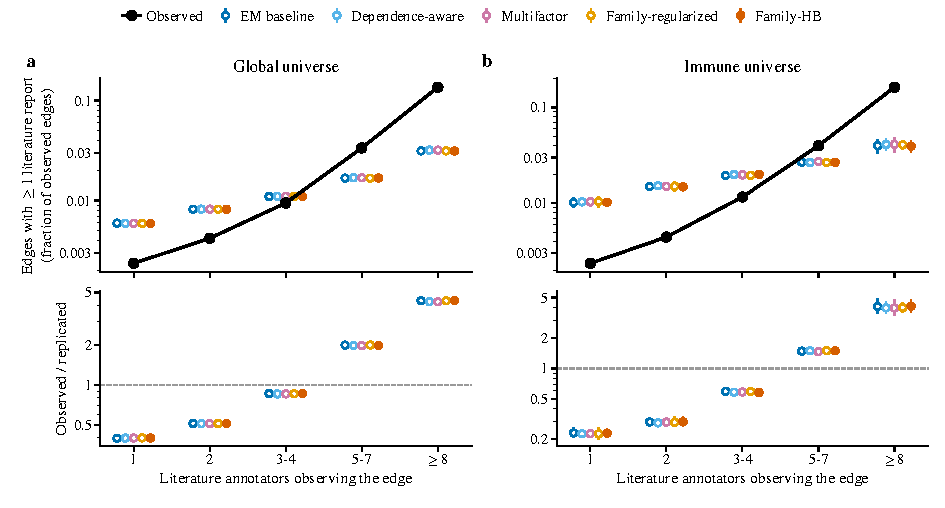
\includegraphics[width=\textwidth]{figS1_ppc.pdf}
  \caption{\textbf{Posterior predictive check of the literature block.} For edges observed by a given number of literature annotators (x axis), the fraction with at least one literature report: observed (black) and the mean over 20 data sets replicated from each fitted estimator on the real observation masks (coloured; bars: mean $\pm 1.96$ replicate SD). Lower panels: observed divided by replicated (reference line at 1). Every estimator, including Family-HB, under-predicts the reporting rate of edges observed by many annotators and over-predicts it for edges observed by few (inference: observation is not ignorable).}
  \label{fig:S-ppc}
\end{figure}

% provenance: paper/r2/tables/tabS_recovery.tex generated by src/r2/paper_assets on 2026-10-15 04:06 from data/r2/tables/
%   fit_recovery.csv (modified 2026-10-14 20:12): simulator in {faithful_cc, faithful_cc_strat, fixed_masks}; kinds parameter, parameter_by_mode, credibility, realised_fdr, realised_fdr_by_mode, identifiability; family == all
%   modes_faithful_design.csv (modified 2026-10-14 20:12): quantity == n_edges_cc_observed & sim_label in {immune_cc, global_cc}: ratio_sim_mean_to_real
\begin{table}[htbp]
\centering
\small
\setlength{\tabcolsep}{2.4pt}
\caption{Simulation-based recovery at the fitted Family-HB parameters (data simulated from the fitted model and refitted; design-faithful simulator primary, two simulators of the observation design as sensitivity analyses): parameter recovery (mean over annotators), ranking and calibration of credibility, and the realised false discovery rate of the Strong set; Family-HB also by the posterior mode its multi-start MAP selected (truth start: Family-HB started at the true parameters).}
\label{tab:S-recovery}
\begin{tabular}{@{}lccccccccr@{}}
\toprule
 & $w_{\mathrm T}$ & $\alpha$ & $\beta$ & \multicolumn{3}{c}{Credibility} & \multicolumn{3}{c}{Strong set$^{\dagger}$} \\
\cmidrule(lr){5-7}\cmidrule(lr){8-10}
Estimator & bias & RMSE & RMSE & AUROC & Spearman & ECE$^{\dagger}$ & claimed & realised & $n$ \\
\midrule
\multicolumn{10}{@{}l}{\emph{Design-faithful (primary), global universe: 5 replicates, competing mode in 0$^{\dagger}$}} \\
Oracle posterior & -- & -- & -- & 0.866 & 1.000 & 0.001 & 0.050 & 0.052 & 1{,}537 \\
Family-HB, truth start & $-5.6\times 10^{-5}$ & 0.071 & 0.0039 & 0.866 & 0.992 & 0.006 & 0.050 & 0.057 & 1{,}572 \\
Family-HB (MAP) & $-5.6\times 10^{-5}$ & 0.071 & 0.0039 & 0.866 & 0.992 & 0.006 & 0.050 & 0.057 & 1{,}572 \\
\quad truth mode ($n$ = 5) & $-5.6\times 10^{-5}$ & 0.071 & 0.0039 & -- & -- & -- & -- & 0.057 & 1{,}572 \\
EM baseline & 0.0036 & 0.184 & 0.0094 & 0.856 & 0.819 & 0.405 & 0.005 & 0.575 & 8{,}337 \\
\addlinespace[3pt]
\multicolumn{10}{@{}l}{\emph{Design-faithful (primary), immune universe: 20 replicates, competing mode in 2$^{\dagger}$}} \\
Oracle posterior & -- & -- & -- & 0.911 & 1.000 & 0.003 & 0.049 & 0.052 & 142 \\
Family-HB, truth start & $-2.9\times 10^{-5}$ & 0.112 & 0.0067 & 0.911 & 0.994 & 0.013 & 0.049 & 0.062 & 144 \\
Family-HB (MAP) & $3.6\times 10^{-4}$ & 0.145 & 0.0076 & 0.907 & 0.974 & 0.066 & 0.049 & 0.149 & 151 \\
\quad truth mode ($n$ = 18) & $-3.3\times 10^{-5}$ & 0.113 & 0.0068 & -- & -- & -- & -- & 0.060 & 146 \\
\quad competing mode ($n$ = 2) & 0.0038 & 0.309 & 0.013 & -- & -- & -- & -- & 0.944 & 199 \\
EM baseline & 0.0094 & 0.197 & 0.0097 & 0.900 & 0.867 & 0.469 & 0.030 & 0.621 & 895 \\
\addlinespace[3pt]
\multicolumn{10}{@{}l}{\emph{Stratum-specific weights (sensitivity), global universe: 5 replicates, competing mode in 0$^{\dagger}$}} \\
Oracle posterior & -- & -- & -- & 0.904 & 1.000 & 0.001 & 0.050 & 0.049 & 4{,}509 \\
Family-HB, truth start & 0.0018 & 0.053 & 0.0028 & 0.894 & 0.851 & 0.039 & 0.048 & 0.065 & 4{,}244 \\
Family-HB (MAP) & 0.0018 & 0.053 & 0.0028 & 0.894 & 0.851 & 0.039 & 0.048 & 0.065 & 4{,}244 \\
\quad truth mode ($n$ = 5) & 0.0018 & 0.053 & 0.0028 & -- & -- & -- & -- & 0.065 & 4{,}244 \\
EM baseline & 0.0063 & 0.184 & 0.0098 & 0.896 & 0.828 & 0.468 & 0.048 & 0.643 & 22{,}962 \\
\addlinespace[3pt]
\multicolumn{10}{@{}l}{\emph{Stratum-specific weights (sensitivity), immune universe: 20 replicates, competing mode in 0$^{\dagger}$}} \\
Oracle posterior & -- & -- & -- & 0.948 & 1.000 & 0.004 & 0.050 & 0.051 & 380 \\
Family-HB, truth start & 0.0025 & 0.075 & 0.0059 & 0.940 & 0.893 & 0.053 & 0.049 & 0.105 & 364 \\
Family-HB (MAP) & 0.0025 & 0.075 & 0.0059 & 0.940 & 0.893 & 0.053 & 0.049 & 0.105 & 364 \\
\quad truth mode ($n$ = 20) & 0.0025 & 0.075 & 0.0059 & -- & -- & -- & -- & 0.105 & 364 \\
EM baseline & 0.013 & 0.189 & 0.010 & 0.936 & 0.771 & 0.491 & 0.049 & 0.626 & 1{,}512 \\
\addlinespace[3pt]
\multicolumn{10}{@{}l}{\emph{Fixed observation masks (sensitivity), global universe: 5 replicates, competing mode in 1}} \\
Oracle posterior & -- & -- & -- & 0.866 & 1.000 & 0.002 & 0.050 & 0.045 & 1{,}471 \\
Family-HB (MAP) & $1.5\times 10^{-4}$ & 0.148 & 0.0040 & 0.861 & 0.947 & 0.080 & 0.049 & 0.227 & 1{,}416 \\
\quad truth mode ($n$ = 4) & $-4.0\times 10^{-5}$ & 0.043 & 0.0042 & -- & -- & -- & -- & 0.046 & 1{,}436 \\
\quad competing mode ($n$ = 1) & $9.3\times 10^{-4}$ & 0.320 & 0.0030 & -- & -- & -- & -- & 0.953 & 1{,}334 \\
EM baseline & 0.0035 & 0.177 & 0.0097 & 0.856 & 0.819 & 0.402 & 0.005 & 0.574 & 8{,}223 \\
\addlinespace[3pt]
\multicolumn{10}{@{}l}{\emph{Fixed observation masks (sensitivity), immune universe: 20 replicates, competing mode in 4}} \\
Oracle posterior & -- & -- & -- & 0.911 & 1.000 & 0.005 & 0.049 & 0.055 & 138 \\
Family-HB (MAP) & $3.4\times 10^{-4}$ & 0.192 & 0.0051 & 0.901 & 0.952 & 0.111 & 0.048 & 0.230 & 155 \\
\quad truth mode ($n$ = 16) & $-4.1\times 10^{-4}$ & 0.143 & 0.0052 & -- & -- & -- & -- & 0.055 & 135 \\
\quad competing mode ($n$ = 4) & 0.0034 & 0.320 & 0.0049 & -- & -- & -- & -- & 0.932 & 235 \\
EM baseline & 0.0087 & 0.197 & 0.0097 & 0.901 & 0.866 & 0.454 & 0.017 & 0.600 & 765 \\
\bottomrule
\end{tabular}
\par\smallskip
\begin{minipage}{\linewidth}\footnotesize
Bias of $w_{\mathrm T}$ and root-mean-square error (RMSE) of the annotator rates $\alpha$ and $\beta$ on the probability scale (oracle: true parameters, --). ECE: expected calibration error over credibility bins 0.1--0.9, pooled over replicates. Strong set: BFDR\,$\le$\,0.05; claimed: its posterior expected FDR; realised: share of simulated non-edges in it. Competing mode: replicates whose selected optimum is not the truth-aligned one; the by-mode rows have few replicates. Design-faithful: real literature observation masks, motif and coexpression masks rebuilt from the simulated literature reports as in the evidence builder. Its data contain 59\% (immune) and 62\% (global) of the real number of motif- or coexpression-observed edges, i.e. fewer informative observations than the real data. Stratum-specific: the same with class weights that depend on the literature-mask stratum, which reproduces the real literature report counts. Fixed masks: every observation mask fixed at the real one, so that motif and coexpression observations do not depend on the simulated literature reports.

$^{\dagger}$\,Post hoc: defined after the held-out data had been examined.
\end{minipage}
\end{table}

% generated by src/r2/paper_assets (make_paper_assets.py figures); do not edit by hand
% provenance: figS7_recovery_calibration generated by src/r2/paper_assets on 2026-10-15 04:07 from data/r2/tables/
%   fit_recovery_calibration.csv (modified 2026-10-14 20:12): in_ece_bins1_9 == True (bins 1-9); all estimators; simulator = faithful_cc (design-faithful)
%   fit_recovery.csv (modified 2026-10-14 20:12): simulator = faithful_cc: analysis_status of the truth-start estimator and of quantity ece_bins1_9 (post hoc flags)
%   modes_faithful_design.csv (modified 2026-10-14 20:12): quantity = n_edges_cc_observed, sim_label in {immune_cc, global_cc}: ratio_sim_mean_to_real
\begin{figure}[htbp]
  \centering
  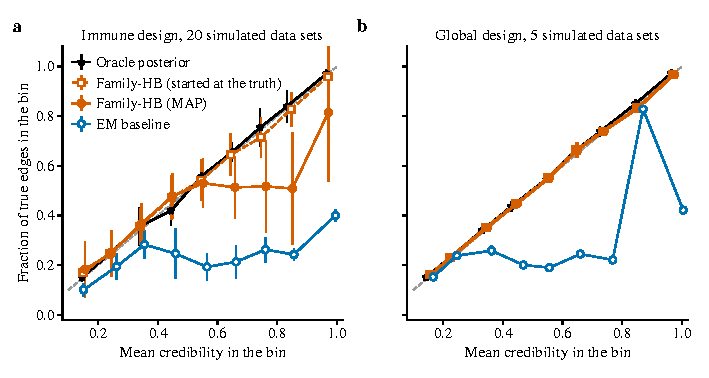
\includegraphics[width=0.75\textwidth]{figS7_recovery_calibration.pdf}
  \caption{\textbf{Calibration of credibility in simulation.} Data simulated from the fitted Family-HB model with the real literature observation masks and the motif/coexpression masks rebuilt from the simulated literature reports (design-faithful simulator; the simulated data contain 59\% (immune) and 62\% (global) of the real number of motif- or coexpression-observed edges). Edges are binned by credibility (bins from 0.1 to 1; the bin below 0.1, which holds almost all edges, is omitted); points: pooled fraction of truly regulatory edges against the mean credibility in the bin; bars: $\pm 1$ SD of that fraction across simulated data sets; dashed line: perfect calibration. Started at the true parameters, Family-HB is close to the oracle posterior; multi-start MAP selects the competing mode in some data sets (immune 2 of 20, global 0 of 5), which pulls the upper bins down and widens their spread; the EM baseline is over-confident (fraction of true edges more than 0.01 below the mean credibility) in 16 of its 18 universe $\times$ bin cells. The design-faithful simulation is post hoc (defined after the held-out data had been examined; it uses no held-out data).}
  \label{fig:S-recovery}
\end{figure}

% provenance: paper/r2/tables/tabS_modes_sim.tex generated by src/r2/paper_assets on 2026-10-15 04:06 from data/r2/tables/
%   modes_simulation.csv (modified 2026-10-14 20:12): simulator in {faithful_cc, faithful_cc_strat, fixed_masks}; stratum in {all, real_gap_<u>, gap_ge_real_<u>, logistic_at_real_gap_<u>}
%   modes_simulation_replicates.csv (modified 2026-10-14 20:12): simulator == faithful_cc: replicates whose Laplace-mixture Strong set is empty (mixture_laplace_strong_n == 0) and dominant_is_truth
%   modes_faithful_design.csv (modified 2026-10-14 20:12): quantity == n_edges_cc_observed & sim_label in {immune_cc, global_cc}: ratio_sim_mean_to_real
\begin{table}[htbp]
\centering
\small
\caption{Mode-selection simulation: data simulated from the dominant Family-HB optimum (truth = dominant mode) or, in the immune universe, from the second optimum (truth = second mode), refitted by multi-start MAP; how often the highest-posterior optimum is the truth, how the gap between the two optima compares with the real gaps, and what the Strong set of each optimum realises. Rows by simulator of the observation design.$^{\dagger}$}
\label{tab:S-modes-sim}
\begin{tabular}{@{}lccc@{}}
\toprule
 & Global & Immune & Immune, truth = \\
 &  &  & second mode \\
\midrule
\multicolumn{4}{@{}l}{\emph{Design-faithful simulator (primary)}} \\
Replicates & 20 & 100 & 30 \\
P(dominant optimum = truth) & \begin{tabular}[t]{@{}c@{}}1.00\\[-1pt]{\scriptsize [0.84, 1.00]}\end{tabular} & \begin{tabular}[t]{@{}c@{}}0.93\\[-1pt]{\scriptsize [0.86, 0.97]}\end{tabular} & \begin{tabular}[t]{@{}c@{}}0.60\\[-1pt]{\scriptsize [0.42, 0.75]}\end{tabular} \\
P(truth optimum found) & \begin{tabular}[t]{@{}c@{}}1.00\\[-1pt]{\scriptsize [0.84, 1.00]}\end{tabular} & \begin{tabular}[t]{@{}c@{}}1.00\\[-1pt]{\scriptsize [0.96, 1.00]}\end{tabular} & \begin{tabular}[t]{@{}c@{}}1.00\\[-1pt]{\scriptsize [0.89, 1.00]}\end{tabular} \\
Median gap between the two optima (nats) & \begin{tabular}[t]{@{}c@{}}49.8\\[-1pt]{\scriptsize [32.6, 63.4]}\end{tabular} & \begin{tabular}[t]{@{}c@{}}4.6\\[-1pt]{\scriptsize [1.2, 8.3]}\end{tabular} & \begin{tabular}[t]{@{}c@{}}1.6\\[-1pt]{\scriptsize [0.2, 3.8]}\end{tabular} \\
Share of simulated gaps below the real gap$^{g}$ & 1.00 & 0.84 & 1.00 \\
Mean Laplace probability of the other optimum & $4.7\times 10^{-14}$ & 0.12 & 0.24 \\
Strong realised FDR, dominant optimum & \begin{tabular}[t]{@{}c@{}}0.054\\[-1pt]{\scriptsize [0.036, 0.064]}\end{tabular} & \begin{tabular}[t]{@{}c@{}}0.125\\[-1pt]{\scriptsize [0.025, 0.140]}\end{tabular} & \begin{tabular}[t]{@{}c@{}}0.415\\[-1pt]{\scriptsize [0.042, 0.962]}\end{tabular} \\
P(realised FDR $>$ 0.10), dominant & 0.00 & 0.22 & 0.43 \\
Strong realised FDR, truth-start & \begin{tabular}[t]{@{}c@{}}0.054\\[-1pt]{\scriptsize [0.036, 0.064]}\end{tabular} & \begin{tabular}[t]{@{}c@{}}0.065\\[-1pt]{\scriptsize [0.025, 0.118]}\end{tabular} & \begin{tabular}[t]{@{}c@{}}0.067\\[-1pt]{\scriptsize [0.036, 0.096]}\end{tabular} \\
Strong realised FDR, other optimum & \begin{tabular}[t]{@{}c@{}}0.945\\[-1pt]{\scriptsize [0.930, 0.961]}\end{tabular} & \begin{tabular}[t]{@{}c@{}}0.869\\[-1pt]{\scriptsize [0.857, 0.967]}\end{tabular} & \begin{tabular}[t]{@{}c@{}}0.593\\[-1pt]{\scriptsize [0.055, 0.960]}\end{tabular} \\
Strong realised FDR, Laplace mixture & \begin{tabular}[t]{@{}c@{}}0.054\\[-1pt]{\scriptsize [0.036, 0.064]}\end{tabular} & \begin{tabular}[t]{@{}c@{}}0.051\\[-1pt]{\scriptsize [0.000, 0.111] $n$ = 67}\end{tabular} & \begin{tabular}[t]{@{}c@{}}0.295\\[-1pt]{\scriptsize [0.000, 0.990] $n$ = 13}\end{tabular} \\
Strong realised FDR, oracle & \begin{tabular}[t]{@{}c@{}}0.051\\[-1pt]{\scriptsize [0.041, 0.058]}\end{tabular} & \begin{tabular}[t]{@{}c@{}}0.050\\[-1pt]{\scriptsize [0.030, 0.072]}\end{tabular} & \begin{tabular}[t]{@{}c@{}}0.052\\[-1pt]{\scriptsize [0.036, 0.075]}\end{tabular} \\
Strong realised FDR, EM & \begin{tabular}[t]{@{}c@{}}0.572\\[-1pt]{\scriptsize [0.563, 0.581]}\end{tabular} & \begin{tabular}[t]{@{}c@{}}0.611\\[-1pt]{\scriptsize [0.565, 0.665]}\end{tabular} & \begin{tabular}[t]{@{}c@{}}0.434\\[-1pt]{\scriptsize [0.398, 0.473]}\end{tabular} \\
P(truth ahead by $\geq$ 7.5 nats, immune) & \begin{tabular}[t]{@{}c@{}}1.00\\[-1pt]{\scriptsize [0.84, 1.00]}\end{tabular} & \begin{tabular}[t]{@{}c@{}}0.16\\[-1pt]{\scriptsize [0.10, 0.24]}\end{tabular} & \begin{tabular}[t]{@{}c@{}}0.00\\[-1pt]{\scriptsize [0.00, 0.11]}\end{tabular} \\
P(other ahead by $\geq$ 7.5 nats, immune) & \begin{tabular}[t]{@{}c@{}}0.00\\[-1pt]{\scriptsize [0.00, 0.16]}\end{tabular} & \begin{tabular}[t]{@{}c@{}}0.00\\[-1pt]{\scriptsize [0.00, 0.04]}\end{tabular} & \begin{tabular}[t]{@{}c@{}}0.00\\[-1pt]{\scriptsize [0.00, 0.11]}\end{tabular} \\
P(dominant = truth $\mid$ gap $\geq$ 7.5, immune) & \begin{tabular}[t]{@{}c@{}}1.00\\[-1pt]{\scriptsize [0.84, 1.00] $n$ = 20}\end{tabular} & \begin{tabular}[t]{@{}c@{}}1.00\\[-1pt]{\scriptsize [0.81, 1.00] $n$ = 16}\end{tabular} & -- \\
Logistic P(dominant = truth) at 7.5, immune & -- & \begin{tabular}[t]{@{}c@{}}1.00\\[-1pt]{\scriptsize [0.99, 1.00]}\end{tabular} & (0.79)$^{e}$ \\
P(dominant = truth $\mid$ gap $\geq$ 7.9, kidney) & \begin{tabular}[t]{@{}c@{}}1.00\\[-1pt]{\scriptsize [0.84, 1.00] $n$ = 20}\end{tabular} & \begin{tabular}[t]{@{}c@{}}1.00\\[-1pt]{\scriptsize [0.78, 1.00] $n$ = 14}\end{tabular} & -- \\
Logistic P(dominant = truth) at 7.9, kidney & -- & \begin{tabular}[t]{@{}c@{}}1.00\\[-1pt]{\scriptsize [0.99, 1.00]}\end{tabular} & (0.80)$^{e}$ \\
P(dominant = truth $\mid$ gap $\geq$ 11.6, lung) & \begin{tabular}[t]{@{}c@{}}1.00\\[-1pt]{\scriptsize [0.84, 1.00] $n$ = 20}\end{tabular} & \begin{tabular}[t]{@{}c@{}}1.00\\[-1pt]{\scriptsize [0.34, 1.00] $n$ = 2}\end{tabular} & -- \\
\bottomrule
\end{tabular}
\end{table}

\begin{table}[htbp]
\ContinuedFloat
\centering
\small
\caption{Mode-selection simulation: data simulated from the dominant Family-HB optimum (truth = dominant mode) or, in the immune universe, from the second optimum (truth = second mode), refitted by multi-start MAP; how often the highest-posterior optimum is the truth, how the gap between the two optima compares with the real gaps, and what the Strong set of each optimum realises. Rows by simulator of the observation design.$^{\dagger}$ (continued)}
\label{tab:S-modes-sim-b}
\begin{tabular}{@{}lccc@{}}
\toprule
 & Global & Immune & Immune, truth = \\
 &  &  & second mode \\
\midrule
\multicolumn{4}{@{}l}{\emph{Design-faithful, stratum-specific class weights (sensitivity)}} \\
Replicates & 20 & 100 & 30 \\
P(dominant optimum = truth) & \begin{tabular}[t]{@{}c@{}}1.00\\[-1pt]{\scriptsize [0.84, 1.00]}\end{tabular} & \begin{tabular}[t]{@{}c@{}}1.00\\[-1pt]{\scriptsize [0.96, 1.00]}\end{tabular} & \begin{tabular}[t]{@{}c@{}}0.97\\[-1pt]{\scriptsize [0.83, 0.99]}\end{tabular} \\
Median gap between the two optima (nats) & \begin{tabular}[t]{@{}c@{}}101.1\\[-1pt]{\scriptsize [93.4, 117.0]}\end{tabular} & \begin{tabular}[t]{@{}c@{}}9.6\\[-1pt]{\scriptsize [5.6, 15.4]}\end{tabular} & \begin{tabular}[t]{@{}c@{}}3.3\\[-1pt]{\scriptsize [1.0, 8.9]}\end{tabular} \\
Share of simulated gaps below the real gap$^{g}$ & 0.60 & 0.31 & 0.87 \\
Strong realised FDR, dominant optimum & \begin{tabular}[t]{@{}c@{}}0.061\\[-1pt]{\scriptsize [0.049, 0.079]}\end{tabular} & \begin{tabular}[t]{@{}c@{}}0.095\\[-1pt]{\scriptsize [0.060, 0.136]}\end{tabular} & \begin{tabular}[t]{@{}c@{}}0.097\\[-1pt]{\scriptsize [0.048, 0.103]}\end{tabular} \\
Strong realised FDR, other optimum & \begin{tabular}[t]{@{}c@{}}0.941\\[-1pt]{\scriptsize [0.937, 0.947]}\end{tabular} & \begin{tabular}[t]{@{}c@{}}0.954\\[-1pt]{\scriptsize [0.936, 0.972]}\end{tabular} & \begin{tabular}[t]{@{}c@{}}0.928\\[-1pt]{\scriptsize [0.935, 0.975]}\end{tabular} \\
Strong realised FDR, oracle & \begin{tabular}[t]{@{}c@{}}0.049\\[-1pt]{\scriptsize [0.046, 0.054]}\end{tabular} & \begin{tabular}[t]{@{}c@{}}0.051\\[-1pt]{\scriptsize [0.037, 0.065]}\end{tabular} & \begin{tabular}[t]{@{}c@{}}0.050\\[-1pt]{\scriptsize [0.041, 0.060]}\end{tabular} \\
P(truth ahead by $\geq$ 7.5 nats, immune) & \begin{tabular}[t]{@{}c@{}}1.00\\[-1pt]{\scriptsize [0.84, 1.00]}\end{tabular} & \begin{tabular}[t]{@{}c@{}}0.69\\[-1pt]{\scriptsize [0.59, 0.77]}\end{tabular} & \begin{tabular}[t]{@{}c@{}}0.13\\[-1pt]{\scriptsize [0.05, 0.30]}\end{tabular} \\
P(other ahead by $\geq$ 7.5 nats, immune) & \begin{tabular}[t]{@{}c@{}}0.00\\[-1pt]{\scriptsize [0.00, 0.16]}\end{tabular} & \begin{tabular}[t]{@{}c@{}}0.00\\[-1pt]{\scriptsize [0.00, 0.04]}\end{tabular} & \begin{tabular}[t]{@{}c@{}}0.00\\[-1pt]{\scriptsize [0.00, 0.11]}\end{tabular} \\
P(dominant = truth $\mid$ gap $\geq$ 108.3, global) & \begin{tabular}[t]{@{}c@{}}1.00\\[-1pt]{\scriptsize [0.68, 1.00] $n$ = 8}\end{tabular} & -- & -- \\
P(dominant = truth $\mid$ gap $\geq$ 7.5, immune) & \begin{tabular}[t]{@{}c@{}}1.00\\[-1pt]{\scriptsize [0.84, 1.00] $n$ = 20}\end{tabular} & \begin{tabular}[t]{@{}c@{}}1.00\\[-1pt]{\scriptsize [0.95, 1.00] $n$ = 69}\end{tabular} & \begin{tabular}[t]{@{}c@{}}1.00\\[-1pt]{\scriptsize [0.51, 1.00] $n$ = 4}\end{tabular} \\
P(dominant = truth $\mid$ gap $\geq$ 7.9, kidney) & \begin{tabular}[t]{@{}c@{}}1.00\\[-1pt]{\scriptsize [0.84, 1.00] $n$ = 20}\end{tabular} & \begin{tabular}[t]{@{}c@{}}1.00\\[-1pt]{\scriptsize [0.94, 1.00] $n$ = 66}\end{tabular} & \begin{tabular}[t]{@{}c@{}}1.00\\[-1pt]{\scriptsize [0.51, 1.00] $n$ = 4}\end{tabular} \\
P(dominant = truth $\mid$ gap $\geq$ 11.6, lung) & \begin{tabular}[t]{@{}c@{}}1.00\\[-1pt]{\scriptsize [0.84, 1.00] $n$ = 20}\end{tabular} & \begin{tabular}[t]{@{}c@{}}1.00\\[-1pt]{\scriptsize [0.88, 1.00] $n$ = 29}\end{tabular} & -- \\
\bottomrule
\end{tabular}
\end{table}

\begin{table}[htbp]
\ContinuedFloat
\centering
\small
\caption{Mode-selection simulation: data simulated from the dominant Family-HB optimum (truth = dominant mode) or, in the immune universe, from the second optimum (truth = second mode), refitted by multi-start MAP; how often the highest-posterior optimum is the truth, how the gap between the two optima compares with the real gaps, and what the Strong set of each optimum realises. Rows by simulator of the observation design.$^{\dagger}$ (continued)}
\label{tab:S-modes-sim-c}
\begin{tabular}{@{}lccc@{}}
\toprule
 & Global & Immune & Immune, truth = \\
 &  &  & second mode \\
\midrule
\multicolumn{4}{@{}l}{\emph{Fixed observation masks (sensitivity)}} \\
Replicates & 10 & 100 & 30 \\
P(dominant optimum = truth) & \begin{tabular}[t]{@{}c@{}}0.70\\[-1pt]{\scriptsize [0.40, 0.89]}\end{tabular} & \begin{tabular}[t]{@{}c@{}}0.68\\[-1pt]{\scriptsize [0.58, 0.76]}\end{tabular} & \begin{tabular}[t]{@{}c@{}}0.77\\[-1pt]{\scriptsize [0.59, 0.88]}\end{tabular} \\
Median gap between the two optima (nats) & \begin{tabular}[t]{@{}c@{}}3.7\\[-1pt]{\scriptsize [2.4, 6.0]}\end{tabular} & \begin{tabular}[t]{@{}c@{}}0.8\\[-1pt]{\scriptsize [0.1, 3.4]}\end{tabular} & \begin{tabular}[t]{@{}c@{}}1.1\\[-1pt]{\scriptsize [0.3, 2.5]}\end{tabular} \\
Share of simulated gaps below the real gap$^{g}$ & 1.00 & 0.98 & 1.00 \\
Strong realised FDR, dominant optimum & \begin{tabular}[t]{@{}c@{}}0.319\\[-1pt]{\scriptsize [0.046, 0.939]}\end{tabular} & \begin{tabular}[t]{@{}c@{}}0.338\\[-1pt]{\scriptsize [0.026, 0.952]}\end{tabular} & \begin{tabular}[t]{@{}c@{}}0.279\\[-1pt]{\scriptsize [0.058, 0.951]}\end{tabular} \\
Strong realised FDR, other optimum & \begin{tabular}[t]{@{}c@{}}0.683\\[-1pt]{\scriptsize [0.052, 0.962]}\end{tabular} & \begin{tabular}[t]{@{}c@{}}0.656\\[-1pt]{\scriptsize [0.035, 0.967] $n$ = 99}\end{tabular} & \begin{tabular}[t]{@{}c@{}}0.740\\[-1pt]{\scriptsize [0.068, 0.974]}\end{tabular} \\
Strong realised FDR, oracle & \begin{tabular}[t]{@{}c@{}}0.050\\[-1pt]{\scriptsize [0.045, 0.059]}\end{tabular} & \begin{tabular}[t]{@{}c@{}}0.051\\[-1pt]{\scriptsize [0.028, 0.073]}\end{tabular} & \begin{tabular}[t]{@{}c@{}}0.053\\[-1pt]{\scriptsize [0.034, 0.069]}\end{tabular} \\
P(truth ahead by $\geq$ 7.5 nats, immune) & \begin{tabular}[t]{@{}c@{}}0.10\\[-1pt]{\scriptsize [0.02, 0.40]}\end{tabular} & \begin{tabular}[t]{@{}c@{}}0.01\\[-1pt]{\scriptsize [0.00, 0.05]}\end{tabular} & \begin{tabular}[t]{@{}c@{}}0.00\\[-1pt]{\scriptsize [0.00, 0.11]}\end{tabular} \\
P(other ahead by $\geq$ 7.5 nats, immune) & \begin{tabular}[t]{@{}c@{}}0.00\\[-1pt]{\scriptsize [0.00, 0.28]}\end{tabular} & \begin{tabular}[t]{@{}c@{}}0.00\\[-1pt]{\scriptsize [0.00, 0.04]}\end{tabular} & \begin{tabular}[t]{@{}c@{}}0.00\\[-1pt]{\scriptsize [0.00, 0.11]}\end{tabular} \\
P(dominant = truth $\mid$ gap $\geq$ 7.5, immune) & \begin{tabular}[t]{@{}c@{}}1.00\\[-1pt]{\scriptsize [0.21, 1.00] $n$ = 1}\end{tabular} & \begin{tabular}[t]{@{}c@{}}0.50\\[-1pt]{\scriptsize [0.09, 0.91] $n$ = 2}\end{tabular} & -- \\
P(dominant = truth $\mid$ gap $\geq$ 7.9, kidney) & -- & \begin{tabular}[t]{@{}c@{}}0.00\\[-1pt]{\scriptsize [0.00, 0.79] $n$ = 1}\end{tabular} & -- \\
P(dominant = truth $\mid$ gap $\geq$ 11.6, lung) & -- & \begin{tabular}[t]{@{}c@{}}0.00\\[-1pt]{\scriptsize [0.00, 0.79] $n$ = 1}\end{tabular} & -- \\
\bottomrule
\end{tabular}
\par\smallskip
\begin{minipage}{\linewidth}\footnotesize
Design-faithful: real literature observation masks, motif and coexpression masks rebuilt from the simulated literature reports as in the evidence builder. Its data contain 59\% (immune) and 62\% (global) of the real number of motif- or coexpression-observed edges, i.e. fewer informative observations than the real data. Stratum-specific: the same with class weights that depend on the literature-mask stratum, which reproduces the real literature report counts. Fixed masks: every observation mask fixed at the real one, so that motif and coexpression observations do not depend on the simulated literature reports.

$^{g}$\,Real gap of the simulated universe: 108.3 nats (global), 7.5 nats (immune); the immune columns use the immune gap.

Laplace mixture: replicates whose mixture Strong set is empty are omitted ($n$: replicates used; immune, 33 of 100 omitted, among them 7 of the 7 replicates in which the wrong optimum is dominant; dominant optimum on the replicates used 0.062; truth = second mode, 17 of 30 omitted, among them 8 of the 12 replicates in which the wrong optimum is dominant; dominant optimum on the replicates used 0.342): the mixture abstains rather than errs in the omitted replicates, so its realised FDR is not comparable with the dominant-optimum row over all replicates.

Intervals: probabilities, Wilson 95\% interval (logistic rows: Wald 95\%); medians and means, 10th--90th percentile over replicates. Gaps: real log-posterior gaps of the fitted universes (global, immune, kidney, lung). Truth-start: fit started at the true parameters; other optimum: the next-best optimum of the same fit; Laplace mixture: credibility averaged over the optima with Laplace weights.

$^{e}$\,Extrapolated (flagged in the source table): too few replicates reach that gap, so the logistic curve is evaluated beyond the simulated gaps (no interval); rows in which every cell is extrapolated are omitted.

$^{\dagger}$\,Post hoc: defined after the held-out data had been examined.
\end{minipage}
\end{table}

% provenance: paper/r2/tables/tabS_modes_gov.tex generated by src/r2/paper_assets on 2026-10-15 04:06 from data/r2/tables/
%   modes_governance_sensitivity.csv (modified 2026-10-14 20:11): all rows
\begin{table}[htbp]
\centering
\small
\setlength{\tabcolsep}{3pt}
\caption{Governance under a two-mode mixture posterior: credibility averaged over the dominant and the second Family-HB mode with second-mode weight $p_2$ (bridge-sampling estimate, its upper Monte-Carlo bound, the Laplace estimate, or fixed values), tier sizes, Jaccard index with the primary sets, and the posterior expected FDR of the primary dual Strong and promoted sets under the mixture.$^{\dagger}$}
\label{tab:S-modes-gov}
\begin{tabular}{@{}lccrrrcccc@{}}
\toprule
 & \multicolumn{2}{c}{$p_2$} & \multicolumn{3}{c}{Tier size (dual)} & \multicolumn{2}{c}{Jaccard} & \multicolumn{2}{c}{FDR of primary} \\
\cmidrule(lr){2-3}\cmidrule(lr){4-6}\cmidrule(lr){7-8}\cmidrule(lr){9-10}
Scenario & ctx. & glob. & ctx.\ Strong & Strong & prom. & Strong & prom. & Strong & prom. \\
\midrule
\multicolumn{10}{@{}l}{\emph{Immune}} \\
dominant mode (primary) & 0 & 0 & 334 & 297 & 493 & 1.00 & 1.00 & 0.036 & 0.159 \\
dominant mode, re-run & 0 & 0 & 333 & 297 & 493 & 1.00 & 1.00 & 0.036 & 0.159 \\
bridge $p_2$ & 0.0044 & $1.8\times 10^{-46}$ & 326 & 296 & 492 & 1.00 & 1.00 & 0.040 & 0.162 \\
bridge, upper bound & 0.0069 & $1.8\times 10^{-46}$ & 321 & 292 & 492 & 0.98 & 1.00 & 0.042 & 0.164 \\
Laplace $p_2$ & 0.0016 & $3.9\times 10^{-46}$ & 331 & 297 & 493 & 1.00 & 1.00 & 0.037 & 0.160 \\
fixed $p_2$ & 0.01 & $1.8\times 10^{-46}$ & 315 & 291 & 490 & 0.98 & 0.99 & 0.045 & 0.166 \\
fixed $p_2$, both fits & 0.01 & 0.01 & 315 & 273 & 484 & 0.92 & 0.98 & 0.045 & 0.166 \\
fixed $p_2$ & 0.05 & $1.8\times 10^{-46}$ & 31 & 31 & 480 & 0.10 & 0.97 & 0.082 & 0.195 \\
fixed $p_2$, both fits & 0.05 & 0.05 & 31 & 27 & 449 & 0.09 & 0.91 & 0.082 & 0.195 \\
fixed $p_2$ & 0.10 & $1.8\times 10^{-46}$ & 0 & 0 & 441 & 0.00 & 0.89 & 0.129 & 0.231 \\
fixed $p_2$, both fits & 0.10 & 0.10 & 0 & 0 & 388 & 0.00 & 0.79 & 0.129 & 0.231 \\
second mode only & 1.00 & $1.8\times 10^{-46}$ & 438 & 0 & 18 & 0.00 & 0.02 & 0.967 & 0.880 \\
\addlinespace[3pt]
\multicolumn{10}{@{}l}{\emph{Kidney}} \\
dominant mode (primary) & 0 & 0 & 179 & 149 & 276 & 1.00 & 1.00 & 0.034 & 0.157 \\
dominant mode, re-run & 0 & 0 & 179 & 149 & 276 & 1.00 & 1.00 & 0.034 & 0.158 \\
bridge $p_2$ & 0.0029 & $1.8\times 10^{-46}$ & 176 & 149 & 276 & 1.00 & 1.00 & 0.037 & 0.159 \\
bridge, upper bound & 0.0048 & $1.8\times 10^{-46}$ & 173 & 148 & 275 & 0.99 & 1.00 & 0.038 & 0.161 \\
Laplace $p_2$ & 0.0073 & $3.9\times 10^{-46}$ & 170 & 148 & 275 & 0.99 & 1.00 & 0.041 & 0.162 \\
fixed $p_2$ & 0.01 & $1.8\times 10^{-46}$ & 166 & 146 & 274 & 0.98 & 0.99 & 0.043 & 0.164 \\
fixed $p_2$, both fits & 0.01 & 0.01 & 166 & 138 & 269 & 0.93 & 0.97 & 0.043 & 0.164 \\
fixed $p_2$ & 0.05 & $1.8\times 10^{-46}$ & 36 & 36 & 261 & 0.24 & 0.95 & 0.081 & 0.194 \\
fixed $p_2$, both fits & 0.05 & 0.05 & 36 & 17 & 244 & 0.11 & 0.88 & 0.081 & 0.194 \\
fixed $p_2$ & 0.10 & $1.8\times 10^{-46}$ & 0 & 0 & 242 & 0.00 & 0.88 & 0.128 & 0.231 \\
fixed $p_2$, both fits & 0.10 & 0.10 & 0 & 0 & 206 & 0.00 & 0.75 & 0.128 & 0.231 \\
second mode only & 1.00 & $1.8\times 10^{-46}$ & 183 & 0 & 11 & 0.00 & 0.03 & 0.971 & 0.897 \\
\addlinespace[3pt]
\multicolumn{10}{@{}l}{\emph{Lung}} \\
dominant mode (primary) & 0 & 0 & 232 & 204 & 412 & 1.00 & 1.00 & 0.041 & 0.167 \\
dominant mode, re-run & 0 & 0 & 233 & 205 & 412 & 1.00 & 1.00 & 0.041 & 0.166 \\
bridge $p_2$ & $6.3\times 10^{-5}$ & $1.8\times 10^{-46}$ & 232 & 204 & 412 & 1.00 & 1.00 & 0.041 & 0.167 \\
bridge, upper bound & $1.0\times 10^{-4}$ & $1.8\times 10^{-46}$ & 232 & 204 & 412 & 1.00 & 1.00 & 0.041 & 0.168 \\
Laplace $p_2$ & $8.9\times 10^{-5}$ & $3.9\times 10^{-46}$ & 232 & 204 & 412 & 1.00 & 1.00 & 0.041 & 0.168 \\
fixed $p_2$ & 0.01 & $1.8\times 10^{-46}$ & 210 & 193 & 411 & 0.95 & 1.00 & 0.051 & 0.175 \\
fixed $p_2$, both fits & 0.01 & 0.01 & 210 & 187 & 409 & 0.92 & 0.99 & 0.051 & 0.175 \\
fixed $p_2$ & 0.05 & $1.8\times 10^{-46}$ & 26 & 26 & 391 & 0.13 & 0.95 & 0.088 & 0.205 \\
fixed $p_2$, both fits & 0.05 & 0.05 & 26 & 22 & 368 & 0.11 & 0.89 & 0.088 & 0.205 \\
fixed $p_2$ & 0.10 & $1.8\times 10^{-46}$ & 0 & 0 & 337 & 0.00 & 0.82 & 0.136 & 0.244 \\
fixed $p_2$, both fits & 0.10 & 0.10 & 0 & 0 & 306 & 0.00 & 0.74 & 0.136 & 0.244 \\
second mode only & 1.00 & $1.8\times 10^{-46}$ & 188 & 0 & 1 & 0.00 & 0.00 & 0.986 & 0.928 \\
\bottomrule
\end{tabular}
\par\smallskip
\begin{minipage}{\linewidth}\footnotesize
$p_2$: weight of the second mode in the context and the global fit (the global fit keeps its own estimate unless marked ``both fits''). Ctx.\ Strong: single-fit Strong set of the context fit; Strong and prom.: dual Strong and promoted sets. FDR: posterior expected FDR of the primary sets under the mixture credibility of the context fit.

$^{\dagger}$\,Post hoc: defined after the held-out data had been examined.
\end{minipage}
\end{table}


\clearpage
\section{Sensitivity analyses and tuning on evaluation data}\label{sec:S-sens}
Fits under alternative priors, evidence variants and family definitions, their held-out performance, and the experiment that tunes configurations on perturbation labels to measure the optimism of such tuning (Section~\ref{sec:res-sensitivity}).
% provenance: paper/r2/tables/tabS_sens_fit.tex generated by src/r2/paper_assets on 2026-10-15 04:06 from data/r2/tables/
%   fit_sensitivity.csv (modified 2026-10-14 19:28): reference == family_hb, Family-HB sensitivity fits
%   fit_sensitivity_modes.csv (modified 2026-10-14 20:12): all rows
\begin{table}[htbp]
\centering
\small
\setlength{\tabcolsep}{4pt}
\caption{Sensitivity of the Family-HB fit (posterior mode) to the evidence variant, the family grouping and the priors, against the primary fit: class weight $w_{\mathrm T}$, Spearman correlation of credibilities over observed edges, size and Jaccard index of the posterior-mode BFDR\,$\le$\,0.05 set, and the posterior-mode structure (distinct optima among the restarts, gap to the second optimum and its Laplace probability).}
\label{tab:S-sens-fit}
\begin{tabular}{@{}lccrcrrc@{}}
\toprule
Fit & $w_{\mathrm T}$ & Spearman & BFDR set $n$ & Jaccard & Optima & Gap$^{\dagger}$ & $P$(2nd)$^{\dagger}$ \\
\midrule
\multicolumn{8}{@{}l}{\emph{Global universe (primary: $w_{\mathrm T}$ = 0.0031, BFDR set 4{,}064 edges)}} \\
Literal observation mask & 0.0038 & 0.939 & 5{,}609 & 0.60 & 3 & 2794.9 & $<10^{-300}$\,$^{u}$ \\
Both endpoints required & 0.0036 & 0.820 & 6{,}127 & 0.58 & 4 & 3144.9 & $<10^{-300}$\,$^{u}$ \\
Both endpoints, curated-cond. & 0.0028 & 0.872 & 4{,}270 & 0.89 & 2 & 137.7 & $2.4\times 10^{-58}$ \\
ChIP family included & 0.0033 & 0.975 & 4{,}561 & 0.88 & 4 & 294.9 & $1.5\times 10^{-128}$ \\
ExTRI and NTNU merged & 0.0027 & 0.949 & 2{,}569 & 0.62 & 3 & 144.6 & $2.6\times 10^{-61}$ \\
Without very large regulons & 0.0030 & 0.945 & 3{,}890 & 0.90 & 3 & 101.3 & $5.1\times 10^{-43}$ \\
Without ChIP-derived LIT & 0.0028 & 0.986 & 3{,}349 & 0.77 & 3 & 121.0 & $6.8\times 10^{-52}$ \\
Literature only$^{a}$ & 0.0031 & 1.000 & 3{,}978 & 0.93 & 1 & -- & -- \\
\addlinespace[2pt]
Singleton families & 0.0068 & 0.816 & 18{,}873 & 0.21 & 1 & -- & -- \\
Lineage families & 0.0044 & 0.890 & 8{,}929 & 0.44 & 2 & 24.3 & $4.0\times 10^{-9}$ \\
Data-driven families & 0.0031 & 1.000 & 4{,}065 & 0.99 & 2 & 250.3 & $1.5\times 10^{-108}$ \\
\addlinespace[2pt]
Scale priors halved & 0.0031 & 1.000 & 4{,}060 & 1.00 & 2 & 109.8 & $5.2\times 10^{-47}$ \\
Scale priors doubled & 0.0031 & 1.000 & 4{,}066 & 1.00 & 2 & 107.2 & $2.1\times 10^{-45}$ \\
Dirichlet(0.5) & 0.0031 & 1.000 & 4{,}056 & 1.00 & 2 & 108.0 & $5.4\times 10^{-46}$ \\
Dirichlet(2) & 0.0031 & 1.000 & 4{,}071 & 1.00 & 2 & 109.1 & $2.0\times 10^{-46}$ \\
\addlinespace[3pt]
\multicolumn{8}{@{}l}{\emph{Immune universe (primary: $w_{\mathrm T}$ = 0.0063, BFDR set 331 edges)}} \\
Literal observation mask & 0.0073 & 0.954 & 476 & 0.69 & 2 & 181.9 & $1.9\times 10^{-80}$ \\
Both endpoints required & 0.0069 & 0.893 & 471 & 0.70 & 2 & 192.7 & $4.4\times 10^{-85}$ \\
Both endpoints, curated-cond. & 0.0054 & 0.913 & 317 & 0.94 & 2 & 10.9 & $9.2\times 10^{-5}$ \\
ChIP family included & 0.0065 & 0.984 & 350 & 0.95 & 3 & 8.9 & $1.4\times 10^{-4}$ \\
ExTRI and NTNU merged & 0.0063 & 0.969 & 290 & 0.84 & 2 & 4.5 & 0.026 \\
Without very large regulons & 0.0064 & 0.985 & 335 & 0.99 & 2 & 8.1 & $8.3\times 10^{-4}$ \\
Without ChIP-derived LIT & 0.0066 & 0.991 & 321 & 0.83 & 2 & 7.6 & $4.4\times 10^{-4}$ \\
Literature only$^{a}$ & 0.0063 & 0.999 & 323 & 0.96 & 1 & -- & -- \\
\addlinespace[2pt]
Singleton families & 0.015 & 0.859 & 1{,}284 & 0.26 & 1 & -- & -- \\
Lineage families & 0.0086 & 0.953 & 593 & 0.53 & 1 & -- & -- \\
Data-driven families & 0.0063 & 1.000 & 331 & 1.00 & 2 & 7.5 & 0.0016 \\
\addlinespace[2pt]
Scale priors halved & 0.0062 & 1.000 & 327 & 0.99 & 2 & 7.7 & 0.0052 \\
Scale priors doubled & 0.0063 & 1.000 & 334 & 0.99 & 2 & 6.8 & 0.0033 \\
Dirichlet(0.5) & 0.0063 & 1.000 & 331 & 1.00 & 2 & 7.2 & 0.020 \\
Dirichlet(2) & 0.0063 & 1.000 & 332 & 1.00 & 2 & 7.5 & 0.0011 \\
\bottomrule
\end{tabular}
\par\smallskip
\begin{minipage}{\linewidth}\footnotesize
$^{a}$\,With one modality family the true and literature-burst classes are exchangeable; the labelling is not identified. Gap: log-posterior units; -- where all restarts reached one optimum. BFDR set: posterior-mode set (the Strong tier of the governance tables uses NUTS credibility).

$^{u}$\,Below the smallest double-precision number (the Laplace mass underflows at gaps of thousands of nats).

$^{\dagger}$\,Post hoc: defined after the held-out data had been examined.
\end{minipage}
\end{table}

% provenance: paper/r2/tables/tabS_sens_heldout.tex generated by src/r2/paper_assets on 2026-10-15 04:06 from data/r2/tables/
%   heldout_sensitivity_fits.csv (modified 2026-10-14 20:11): eval_set == all_evaluable
%   heldout_estimators.csv (modified 2026-10-14 20:06): eval_subset == all_evaluable & score == family_hb (primary AP lift, as in the main held-out table)
\begin{table}[htbp]
\centering
\small
\caption{Held-out AP lift of the sensitivity fits and its paired difference to the primary Family-HB (MAP) fit (95\% TF-cluster bootstrap interval), all evaluable edges.}
\label{tab:S-sens-heldout}
\begin{tabular}{@{}lccc@{}}
\toprule
Fit & ENCODE TFBS & ENETS2 & Pooled perturbation \\
\midrule
\multicolumn{4}{@{}l}{\emph{Global universe}} \\
Family-HB (MAP), primary fit: AP lift & \begin{tabular}[t]{@{}c@{}}0.96\\[-1pt]{\scriptsize [0.94, 0.98]}\end{tabular} & \begin{tabular}[t]{@{}c@{}}1.59\\[-1pt]{\scriptsize [1.31, 2.00]}\end{tabular} & \begin{tabular}[t]{@{}c@{}}0.94\\[-1pt]{\scriptsize [0.90, 0.98]}\end{tabular} \\
Family-HB (NUTS) & \begin{tabular}[t]{@{}c@{}}0.000\\[-1pt]{\scriptsize [0.000, 0.000]}\end{tabular} & \begin{tabular}[t]{@{}c@{}}0.000\\[-1pt]{\scriptsize [$-$0.002, 0.002]}\end{tabular} & \begin{tabular}[t]{@{}c@{}}0.000\\[-1pt]{\scriptsize [$-$0.0002, 0.000]}\end{tabular} \\
\addlinespace[2pt]
Family-HB (NUTS, random init.)$^{m}$ & \begin{tabular}[t]{@{}c@{}}0.005\\[-1pt]{\scriptsize [0.002, 0.009]}\end{tabular} & \begin{tabular}[t]{@{}c@{}}0.095\\[-1pt]{\scriptsize [$-$0.009, 0.233]}\end{tabular} & \begin{tabular}[t]{@{}c@{}}0.005\\[-1pt]{\scriptsize [$-$0.006, 0.014]}\end{tabular} \\
\addlinespace[2pt]
Literal observation mask & \begin{tabular}[t]{@{}c@{}}0.017\\[-1pt]{\scriptsize [0.004, 0.033]}\end{tabular} & \begin{tabular}[t]{@{}c@{}}0.790\\[-1pt]{\scriptsize [0.545, 1.106]}\end{tabular} & \begin{tabular}[t]{@{}c@{}}0.020\\[-1pt]{\scriptsize [$-$0.021, 0.088]}\end{tabular} \\
Both endpoints required & \begin{tabular}[t]{@{}c@{}}$-$0.031\\[-1pt]{\scriptsize [$-$0.048, $-$0.013]}\end{tabular} & \begin{tabular}[t]{@{}c@{}}0.721\\[-1pt]{\scriptsize [0.491, 1.023]}\end{tabular} & \begin{tabular}[t]{@{}c@{}}0.053\\[-1pt]{\scriptsize [$-$0.002, 0.122]}\end{tabular} \\
Both endpoints, curated-cond. & \begin{tabular}[t]{@{}c@{}}$-$0.009\\[-1pt]{\scriptsize [$-$0.023, 0.004]}\end{tabular} & \begin{tabular}[t]{@{}c@{}}0.022\\[-1pt]{\scriptsize [$-$0.007, 0.057]}\end{tabular} & \begin{tabular}[t]{@{}c@{}}$-$0.002\\[-1pt]{\scriptsize [$-$0.035, 0.027]}\end{tabular} \\
ChIP family included & \begin{tabular}[t]{@{}c@{}}0.051\\[-1pt]{\scriptsize [0.036, 0.069]}\end{tabular} & \begin{tabular}[t]{@{}c@{}}0.549\\[-1pt]{\scriptsize [0.402, 0.756]}\end{tabular} & \begin{tabular}[t]{@{}c@{}}0.029\\[-1pt]{\scriptsize [$-$0.0002, 0.076]}\end{tabular} \\
ExTRI and NTNU merged & \begin{tabular}[t]{@{}c@{}}0.000\\[-1pt]{\scriptsize [$-$0.002, 0.001]}\end{tabular} & \begin{tabular}[t]{@{}c@{}}0.081\\[-1pt]{\scriptsize [0.033, 0.151]}\end{tabular} & \begin{tabular}[t]{@{}c@{}}0.006\\[-1pt]{\scriptsize [0.002, 0.010]}\end{tabular} \\
Without very large regulons & \begin{tabular}[t]{@{}c@{}}0.019\\[-1pt]{\scriptsize [0.012, 0.025]}\end{tabular} & \begin{tabular}[t]{@{}c@{}}$-$0.063\\[-1pt]{\scriptsize [$-$0.139, $-$0.001]}\end{tabular} & \begin{tabular}[t]{@{}c@{}}0.004\\[-1pt]{\scriptsize [$-$0.010, 0.016]}\end{tabular} \\
Without ChIP-derived LIT & \begin{tabular}[t]{@{}c@{}}0.010\\[-1pt]{\scriptsize [0.006, 0.014]}\end{tabular} & \begin{tabular}[t]{@{}c@{}}$-$0.034\\[-1pt]{\scriptsize [$-$0.106, 0.038]}\end{tabular} & \begin{tabular}[t]{@{}c@{}}0.008\\[-1pt]{\scriptsize [$-$0.003, 0.017]}\end{tabular} \\
Literature only & \begin{tabular}[t]{@{}c@{}}0.000\\[-1pt]{\scriptsize [$-$0.0004, 0.000]}\end{tabular} & \begin{tabular}[t]{@{}c@{}}$-$0.056\\[-1pt]{\scriptsize [$-$0.096, $-$0.026]}\end{tabular} & \begin{tabular}[t]{@{}c@{}}$-$0.001\\[-1pt]{\scriptsize [$-$0.003, $-$0.0002]}\end{tabular} \\
\addlinespace[2pt]
Singleton families & \begin{tabular}[t]{@{}c@{}}0.006\\[-1pt]{\scriptsize [0.001, 0.011]}\end{tabular} & \begin{tabular}[t]{@{}c@{}}$-$0.091\\[-1pt]{\scriptsize [$-$0.242, 0.019]}\end{tabular} & \begin{tabular}[t]{@{}c@{}}0.004\\[-1pt]{\scriptsize [$-$0.012, 0.018]}\end{tabular} \\
Lineage families & \begin{tabular}[t]{@{}c@{}}0.005\\[-1pt]{\scriptsize [0.002, 0.008]}\end{tabular} & \begin{tabular}[t]{@{}c@{}}$-$0.049\\[-1pt]{\scriptsize [$-$0.138, 0.024]}\end{tabular} & \begin{tabular}[t]{@{}c@{}}0.002\\[-1pt]{\scriptsize [$-$0.009, 0.011]}\end{tabular} \\
Data-driven families & \begin{tabular}[t]{@{}c@{}}0.000\\[-1pt]{\scriptsize [$-$0.0003, $-$0.000]}\end{tabular} & \begin{tabular}[t]{@{}c@{}}$-$0.011\\[-1pt]{\scriptsize [$-$0.024, $-$0.0004]}\end{tabular} & \begin{tabular}[t]{@{}c@{}}0.000\\[-1pt]{\scriptsize [$-$0.0001, 0.001]}\end{tabular} \\
\addlinespace[2pt]
Scale priors halved & \begin{tabular}[t]{@{}c@{}}0.000\\[-1pt]{\scriptsize [0.000, 0.000]}\end{tabular} & \begin{tabular}[t]{@{}c@{}}0.002\\[-1pt]{\scriptsize [0.001, 0.005]}\end{tabular} & \begin{tabular}[t]{@{}c@{}}0.000\\[-1pt]{\scriptsize [$-$0.0001, 0.000]}\end{tabular} \\
Scale priors doubled & \begin{tabular}[t]{@{}c@{}}0.000\\[-1pt]{\scriptsize [$-$0.000, $-$0.000]}\end{tabular} & \begin{tabular}[t]{@{}c@{}}$-$0.001\\[-1pt]{\scriptsize [$-$0.002, $-$0.0002]}\end{tabular} & \begin{tabular}[t]{@{}c@{}}0.000\\[-1pt]{\scriptsize [$-$0.0001, 0.000]}\end{tabular} \\
Dirichlet(0.5) & \begin{tabular}[t]{@{}c@{}}0.000\\[-1pt]{\scriptsize [$-$0.000, $-$0.000]}\end{tabular} & \begin{tabular}[t]{@{}c@{}}$-$0.001\\[-1pt]{\scriptsize [$-$0.001, $-$0.0001]}\end{tabular} & \begin{tabular}[t]{@{}c@{}}0.000\\[-1pt]{\scriptsize [$-$0.000, 0.000]}\end{tabular} \\
Dirichlet(2) & \begin{tabular}[t]{@{}c@{}}0.000\\[-1pt]{\scriptsize [$-$0.000, 0.000]}\end{tabular} & \begin{tabular}[t]{@{}c@{}}0.002\\[-1pt]{\scriptsize [0.001, 0.004]}\end{tabular} & \begin{tabular}[t]{@{}c@{}}0.000\\[-1pt]{\scriptsize [$-$0.0001, 0.000]}\end{tabular} \\
\bottomrule
\end{tabular}
\end{table}

\begin{table}[htbp]
\ContinuedFloat
\centering
\small
\caption{Held-out AP lift of the sensitivity fits and its paired difference to the primary Family-HB (MAP) fit (95\% TF-cluster bootstrap interval), all evaluable edges. (continued)}
\label{tab:S-sens-heldout-b}
\begin{tabular}{@{}lccc@{}}
\toprule
Fit & ENCODE TFBS & ENETS2 & Pooled perturbation \\
\midrule
\multicolumn{4}{@{}l}{\emph{Immune universe}} \\
Family-HB (MAP), primary fit: AP lift & \begin{tabular}[t]{@{}c@{}}0.97\\[-1pt]{\scriptsize [0.95, 1.00]}\end{tabular} & \begin{tabular}[t]{@{}c@{}}1.61\\[-1pt]{\scriptsize [1.15, 2.77]}\end{tabular} & \begin{tabular}[t]{@{}c@{}}0.94\\[-1pt]{\scriptsize [0.88, 1.01]}\end{tabular} \\
Family-HB (NUTS) & \begin{tabular}[t]{@{}c@{}}0.001\\[-1pt]{\scriptsize [$-$0.0001, 0.002]}\end{tabular} & \begin{tabular}[t]{@{}c@{}}$-$0.010\\[-1pt]{\scriptsize [$-$0.033, 0.001]}\end{tabular} & \begin{tabular}[t]{@{}c@{}}0.000\\[-1pt]{\scriptsize [$-$0.001, 0.003]}\end{tabular} \\
\addlinespace[2pt]
Family-HB (NUTS, random init.)$^{m}$ & \begin{tabular}[t]{@{}c@{}}0.007\\[-1pt]{\scriptsize [$-$0.002, 0.018]}\end{tabular} & \begin{tabular}[t]{@{}c@{}}$-$0.160\\[-1pt]{\scriptsize [$-$0.825, 0.121]}\end{tabular} & \begin{tabular}[t]{@{}c@{}}$-$0.016\\[-1pt]{\scriptsize [$-$0.035, $-$0.001]}\end{tabular} \\
\addlinespace[2pt]
Literal observation mask & \begin{tabular}[t]{@{}c@{}}0.050\\[-1pt]{\scriptsize [0.018, 0.097]}\end{tabular} & \begin{tabular}[t]{@{}c@{}}0.446\\[-1pt]{\scriptsize [0.077, 0.916]}\end{tabular} & \begin{tabular}[t]{@{}c@{}}$-$0.022\\[-1pt]{\scriptsize [$-$0.062, 0.033]}\end{tabular} \\
Both endpoints required & \begin{tabular}[t]{@{}c@{}}$-$0.008\\[-1pt]{\scriptsize [$-$0.042, 0.039]}\end{tabular} & \begin{tabular}[t]{@{}c@{}}0.329\\[-1pt]{\scriptsize [$-$0.082, 0.788]}\end{tabular} & \begin{tabular}[t]{@{}c@{}}0.017\\[-1pt]{\scriptsize [$-$0.031, 0.079]}\end{tabular} \\
Both endpoints, curated-cond. & \begin{tabular}[t]{@{}c@{}}0.001\\[-1pt]{\scriptsize [$-$0.007, 0.009]}\end{tabular} & \begin{tabular}[t]{@{}c@{}}$-$0.123\\[-1pt]{\scriptsize [$-$0.296, 0.027]}\end{tabular} & \begin{tabular}[t]{@{}c@{}}0.028\\[-1pt]{\scriptsize [0.000, 0.062]}\end{tabular} \\
ChIP family included & \begin{tabular}[t]{@{}c@{}}0.089\\[-1pt]{\scriptsize [0.052, 0.146]}\end{tabular} & \begin{tabular}[t]{@{}c@{}}0.264\\[-1pt]{\scriptsize [0.174, 0.428]}\end{tabular} & \begin{tabular}[t]{@{}c@{}}$-$0.018\\[-1pt]{\scriptsize [$-$0.039, 0.024]}\end{tabular} \\
ExTRI and NTNU merged & \begin{tabular}[t]{@{}c@{}}$-$0.001\\[-1pt]{\scriptsize [$-$0.003, 0.002]}\end{tabular} & \begin{tabular}[t]{@{}c@{}}$-$0.049\\[-1pt]{\scriptsize [$-$0.269, 0.160]}\end{tabular} & \begin{tabular}[t]{@{}c@{}}0.006\\[-1pt]{\scriptsize [$-$0.0001, 0.012]}\end{tabular} \\
Without very large regulons & \begin{tabular}[t]{@{}c@{}}0.005\\[-1pt]{\scriptsize [0.002, 0.008]}\end{tabular} & \begin{tabular}[t]{@{}c@{}}$-$0.072\\[-1pt]{\scriptsize [$-$0.216, 0.027]}\end{tabular} & \begin{tabular}[t]{@{}c@{}}$-$0.004\\[-1pt]{\scriptsize [$-$0.008, 0.001]}\end{tabular} \\
Without ChIP-derived LIT & \begin{tabular}[t]{@{}c@{}}0.001\\[-1pt]{\scriptsize [$-$0.002, 0.006]}\end{tabular} & \begin{tabular}[t]{@{}c@{}}$-$0.178\\[-1pt]{\scriptsize [$-$0.610, 0.021]}\end{tabular} & \begin{tabular}[t]{@{}c@{}}0.003\\[-1pt]{\scriptsize [$-$0.004, 0.011]}\end{tabular} \\
Literature only & \begin{tabular}[t]{@{}c@{}}$-$0.001\\[-1pt]{\scriptsize [$-$0.003, 0.000]}\end{tabular} & \begin{tabular}[t]{@{}c@{}}$-$0.009\\[-1pt]{\scriptsize [$-$0.061, 0.018]}\end{tabular} & \begin{tabular}[t]{@{}c@{}}0.000\\[-1pt]{\scriptsize [$-$0.003, 0.002]}\end{tabular} \\
\addlinespace[2pt]
Singleton families & \begin{tabular}[t]{@{}c@{}}0.007\\[-1pt]{\scriptsize [$-$0.0005, 0.018]}\end{tabular} & \begin{tabular}[t]{@{}c@{}}$-$0.219\\[-1pt]{\scriptsize [$-$0.910, 0.059]}\end{tabular} & \begin{tabular}[t]{@{}c@{}}$-$0.010\\[-1pt]{\scriptsize [$-$0.035, 0.009]}\end{tabular} \\
Lineage families & \begin{tabular}[t]{@{}c@{}}0.005\\[-1pt]{\scriptsize [0.000, 0.011]}\end{tabular} & \begin{tabular}[t]{@{}c@{}}$-$0.152\\[-1pt]{\scriptsize [$-$0.745, 0.154]}\end{tabular} & \begin{tabular}[t]{@{}c@{}}$-$0.004\\[-1pt]{\scriptsize [$-$0.019, 0.006]}\end{tabular} \\
Data-driven families & \begin{tabular}[t]{@{}c@{}}0.000\\[-1pt]{\scriptsize [0.000, 0.000]}\end{tabular} & \begin{tabular}[t]{@{}c@{}}0.000\\[-1pt]{\scriptsize [0.000, 0.000]}\end{tabular} & \begin{tabular}[t]{@{}c@{}}0.000\\[-1pt]{\scriptsize [0.000, 0.000]}\end{tabular} \\
\addlinespace[2pt]
Scale priors halved & \begin{tabular}[t]{@{}c@{}}0.000\\[-1pt]{\scriptsize [$-$0.0001, 0.000]}\end{tabular} & \begin{tabular}[t]{@{}c@{}}0.003\\[-1pt]{\scriptsize [$-$0.002, 0.025]}\end{tabular} & \begin{tabular}[t]{@{}c@{}}0.000\\[-1pt]{\scriptsize [$-$0.0004, 0.002]}\end{tabular} \\
Scale priors doubled & \begin{tabular}[t]{@{}c@{}}0.000\\[-1pt]{\scriptsize [$-$0.0001, 0.001]}\end{tabular} & \begin{tabular}[t]{@{}c@{}}0.002\\[-1pt]{\scriptsize [$-$0.002, 0.016]}\end{tabular} & \begin{tabular}[t]{@{}c@{}}0.000\\[-1pt]{\scriptsize [$-$0.002, 0.000]}\end{tabular} \\
Dirichlet(0.5) & \begin{tabular}[t]{@{}c@{}}0.000\\[-1pt]{\scriptsize [$-$0.000, 0.000]}\end{tabular} & \begin{tabular}[t]{@{}c@{}}0.001\\[-1pt]{\scriptsize [$-$0.0001, 0.002]}\end{tabular} & \begin{tabular}[t]{@{}c@{}}0.000\\[-1pt]{\scriptsize [$-$0.0001, 0.000]}\end{tabular} \\
Dirichlet(2) & \begin{tabular}[t]{@{}c@{}}0.000\\[-1pt]{\scriptsize [$-$0.000, 0.000]}\end{tabular} & \begin{tabular}[t]{@{}c@{}}0.000\\[-1pt]{\scriptsize [$-$0.002, 0.001]}\end{tabular} & \begin{tabular}[t]{@{}c@{}}0.000\\[-1pt]{\scriptsize [$-$0.000, 0.000]}\end{tabular} \\
Scale priors halved (NUTS)$^{m}$ & \begin{tabular}[t]{@{}c@{}}0.008\\[-1pt]{\scriptsize [$-$0.001, 0.020]}\end{tabular} & \begin{tabular}[t]{@{}c@{}}$-$0.159\\[-1pt]{\scriptsize [$-$0.824, 0.126]}\end{tabular} & \begin{tabular}[t]{@{}c@{}}$-$0.016\\[-1pt]{\scriptsize [$-$0.034, $-$0.001]}\end{tabular} \\
Scale priors doubled (NUTS)$^{m}$ & \begin{tabular}[t]{@{}c@{}}0.007\\[-1pt]{\scriptsize [$-$0.002, 0.018]}\end{tabular} & \begin{tabular}[t]{@{}c@{}}$-$0.137\\[-1pt]{\scriptsize [$-$0.820, 0.162]}\end{tabular} & \begin{tabular}[t]{@{}c@{}}$-$0.016\\[-1pt]{\scriptsize [$-$0.035, $-$0.001]}\end{tabular} \\
\bottomrule
\end{tabular}
\par\smallskip
\begin{minipage}{\linewidth}\footnotesize
First row: AP lift of the primary Family-HB (MAP) fit with its 95\% TF-cluster bootstrap interval, as in the main held-out table. Other rows: AP lift of the fit minus AP lift of the primary fit on the same evaluable edges (paired TF-cluster bootstrap of its own).

$^{m}$\,NUTS from random starts whose chains mix posterior modes (maximum $\widehat R$ 1.556--1.742): the difference reflects mode mixing, not the prior or the initialisation.
\end{minipage}
\end{table}

% provenance: paper/r2/tables/tabS_tuning.tex generated by src/r2/paper_assets on 2026-10-15 04:06 from data/r2/tables/
%   tune_optimism.csv (modified 2026-10-14 20:26): fold_set == all_folds; split_type in {random_tf_half, loso}; criterion in {pooled_ap_lift, tf_geomean_ap_lift}
\begin{table}[htbp]
\centering
\small
\setlength{\tabcolsep}{3.5pt}
\caption{Optimism of tuning the configuration on perturbation labels (pooled perturbation reference, global universe): configuration selected on one half of the TFs (or all but one study) and scored on the other, against the label-free choice (best cross-validated log-likelihood) and the fixed primary Family-HB.}
\label{tab:S-tuning}
\begin{tabular}{@{}lp{3.6cm}rrrrrr@{}}
\toprule
Selection & Selected (share) & Distinct & In & Out & Optimism & Out $-$ prim. & $P$ \\
\midrule
\multicolumn{8}{@{}l}{\emph{all configurations (19 configurations), random TF halves (50 splits)}} \\
\multicolumn{8}{@{}l}{\quad Criterion: pooled AP lift} \\
\quad tuned on labels & \parbox[t]{3.6cm}{\raggedright\footnotesize Family-HB, both endpoints required (0.74)} & 4 & 0.994 & 0.979 & 0.015 & 0.040 & 0.94 \\
\quad label-free (CV) & \parbox[t]{3.6cm}{\raggedright\footnotesize Data-driven families (1.00)} & 1 & 0.937 & 0.940 & $-$0.003 & 0.000 & 0.86 \\
\quad primary & \parbox[t]{3.6cm}{\raggedright\footnotesize Family-HB (1.00)} & 1 & 0.937 & 0.940 & $-$0.003 & 0.000 & 0.00 \\
\multicolumn{8}{@{}l}{\quad Criterion: per-TF AP lift (geom.\ mean)} \\
\quad tuned on labels$^{\dagger}$ & \parbox[t]{3.6cm}{\raggedright\footnotesize Family-HB, both endpoints required (0.96)} & 2 & 1.241 & 1.288 & $-$0.047 & 0.097 & 1.00 \\
\quad label-free (CV)$^{\dagger}$ & \parbox[t]{3.6cm}{\raggedright\footnotesize Data-driven families (1.00)} & 1 & 1.152 & 1.196 & $-$0.045 & 0.005 & 0.62 \\
\quad primary$^{\dagger}$ & \parbox[t]{3.6cm}{\raggedright\footnotesize Family-HB (1.00)} & 1 & 1.148 & 1.191 & $-$0.044 & 0.000 & 0.00 \\
\addlinespace[3pt]
\multicolumn{8}{@{}l}{\emph{all configurations (19 configurations), leave one study out (4 splits)}} \\
\multicolumn{8}{@{}l}{\quad Criterion: pooled AP lift} \\
\quad tuned on labels & \parbox[t]{3.6cm}{\raggedright\footnotesize Family-HB, both endpoints required (0.75)} & 2 & 1.007 & 1.020 & $-$0.013 & 0.016 & 0.50 \\
\quad label-free (CV) & \parbox[t]{3.6cm}{\raggedright\footnotesize Data-driven families (1.00)} & 1 & 0.953 & 1.005 & $-$0.052 & 0.001 & 1.00 \\
\quad primary & \parbox[t]{3.6cm}{\raggedright\footnotesize Family-HB (1.00)} & 1 & 0.953 & 1.004 & $-$0.051 & 0.000 & 0.00 \\
\multicolumn{8}{@{}l}{\quad Criterion: per-TF AP lift (geom.\ mean)} \\
\quad tuned on labels$^{\dagger}$ & \parbox[t]{3.6cm}{\raggedright\footnotesize Family-HB, both endpoints required (1.00)} & 1 & 1.271 & 1.440 & $-$0.168 & 0.123 & 1.00 \\
\quad label-free (CV)$^{\dagger}$ & \parbox[t]{3.6cm}{\raggedright\footnotesize Data-driven families (1.00)} & 1 & 1.177 & 1.317 & $-$0.140 & 0.000 & 0.75 \\
\quad primary$^{\dagger}$ & \parbox[t]{3.6cm}{\raggedright\footnotesize Family-HB (1.00)} & 1 & 1.174 & 1.317 & $-$0.143 & 0.000 & 0.00 \\
\addlinespace[3pt]
\multicolumn{8}{@{}l}{\emph{primary evidence only (12 configurations), random TF halves (50 splits)}} \\
\multicolumn{8}{@{}l}{\quad Criterion: pooled AP lift} \\
\quad tuned on labels & \parbox[t]{3.6cm}{\raggedright\footnotesize Data-driven families (0.30)} & 9 & 0.942 & 0.939 & 0.003 & $-$0.001 & 0.54 \\
\quad label-free (CV) & \parbox[t]{3.6cm}{\raggedright\footnotesize Data-driven families (1.00)} & 1 & 0.937 & 0.940 & $-$0.003 & 0.000 & 0.86 \\
\quad primary & \parbox[t]{3.6cm}{\raggedright\footnotesize Family-HB (1.00)} & 1 & 0.937 & 0.940 & $-$0.003 & 0.000 & 0.00 \\
\multicolumn{8}{@{}l}{\quad Criterion: per-TF AP lift (geom.\ mean)} \\
\quad tuned on labels$^{\dagger}$ & \parbox[t]{3.6cm}{\raggedright\footnotesize Lineage families (0.60)} & 6 & 1.162 & 1.191 & $-$0.029 & 0.000 & 0.60 \\
\quad label-free (CV)$^{\dagger}$ & \parbox[t]{3.6cm}{\raggedright\footnotesize Data-driven families (1.00)} & 1 & 1.152 & 1.196 & $-$0.045 & 0.005 & 0.62 \\
\quad primary$^{\dagger}$ & \parbox[t]{3.6cm}{\raggedright\footnotesize Family-HB (1.00)} & 1 & 1.148 & 1.191 & $-$0.044 & 0.000 & 0.00 \\
\addlinespace[3pt]
\multicolumn{8}{@{}l}{\emph{primary evidence only (12 configurations), leave one study out (4 splits)}} \\
\multicolumn{8}{@{}l}{\quad Criterion: pooled AP lift} \\
\quad tuned on labels & \parbox[t]{3.6cm}{\raggedright\footnotesize Singleton families (0.25)} & 4 & 0.958 & 1.061 & $-$0.103 & 0.056 & 1.00 \\
\quad label-free (CV) & \parbox[t]{3.6cm}{\raggedright\footnotesize Data-driven families (1.00)} & 1 & 0.953 & 1.005 & $-$0.052 & 0.001 & 1.00 \\
\quad primary & \parbox[t]{3.6cm}{\raggedright\footnotesize Family-HB (1.00)} & 1 & 0.953 & 1.004 & $-$0.051 & 0.000 & 0.00 \\
\multicolumn{8}{@{}l}{\quad Criterion: per-TF AP lift (geom.\ mean)} \\
\quad tuned on labels$^{\dagger}$ & \parbox[t]{3.6cm}{\raggedright\footnotesize Lineage families (0.75)} & 2 & 1.188 & 1.319 & $-$0.131 & 0.002 & 0.75 \\
\quad label-free (CV)$^{\dagger}$ & \parbox[t]{3.6cm}{\raggedright\footnotesize Data-driven families (1.00)} & 1 & 1.177 & 1.317 & $-$0.140 & 0.000 & 0.75 \\
\quad primary$^{\dagger}$ & \parbox[t]{3.6cm}{\raggedright\footnotesize Family-HB (1.00)} & 1 & 1.174 & 1.317 & $-$0.143 & 0.000 & 0.00 \\
\bottomrule
\end{tabular}
\par\smallskip
\begin{minipage}{\linewidth}\footnotesize
Selected: most frequently selected configuration (share of splits); distinct: number of different configurations selected. In / out: criterion on the tuning / held-out part; optimism: in $-$ out; out $-$ primary: held-out gain over Family-HB; $P$: share of splits with a held-out gain.

$^{\dagger}$\,Post hoc: defined after the held-out data had been examined.
\end{minipage}
\end{table}

% provenance: paper/r2/tables/tabS_tune_status.tex generated by src/r2/paper_assets on 2026-10-15 04:06 from data/r2/tables/
%   tune_status_decomposition.csv (modified 2026-10-14 20:26): all rows
\begin{table}[htbp]
\centering
\small
\setlength{\tabcolsep}{4pt}
\caption{Perturbation positives and credibility by evidence status for every tuning configuration (pooled perturbation reference, global universe): observed over TF-matched expected positives and mean credibility of reported, observed but unreported, and unobserved edges.$^{\dagger}$}
\label{tab:S-tune-status}
\begin{tabular}{@{}lcccccc@{}}
\toprule
Configuration & \multicolumn{2}{c}{Reported} & \multicolumn{2}{c}{Observed, not reported} & \multicolumn{2}{c}{Unobserved} \\
\cmidrule(lr){2-3}\cmidrule(lr){4-5}\cmidrule(lr){6-7}
 & O/E & $\bar c$ & O/E & $\bar c$ & O/E & $\bar c$ \\
\midrule
EM baseline & 1.36 & 0.54 & 1.01 & 0.0023 & 0.97 & 0.0068 \\
Dependence-aware & 1.36 & 0.24 & 1.01 & $5.7\times 10^{-4}$ & 0.97 & 0.0024 \\
Multifactor & 1.36 & 0.029 & 1.01 & $4.5\times 10^{-5}$ & 0.97 & $2.2\times 10^{-4}$ \\
Family-regularized & 1.36 & 0.54 & 1.01 & 0.0023 & 0.97 & 0.0068 \\
Family-HB & 1.36 & 0.24 & 1.01 & 0.0011 & 0.97 & 0.0031 \\
Family-HB, literal observation mask & 1.28 & 0.23 & 1.00 & 0.0017 & 0.96 & 0.0038 \\
Family-HB, both endpoints required & 1.28 & 0.25 & 1.00 & 0.0015 & 0.97 & 0.0036 \\
Family-HB, both endpoints, curated-cond. & 1.36 & 0.26 & 1.00 & 0.0010 & 0.99 & 0.0028 \\
Family-HB, chIP family included & 1.05 & 0.044 & 1.00 & 0.0015 & 0.97 & 0.0033 \\
Family-HB, exTRI and NTNU merged & 1.36 & 0.21 & 1.01 & $9.5\times 10^{-4}$ & 0.97 & 0.0027 \\
Family-HB, without very large regulons & 1.36 & 0.24 & 1.02 & 0.0011 & 0.95 & 0.0030 \\
Family-HB, without ChIP-derived LIT & 1.36 & 0.22 & 1.02 & $9.4\times 10^{-4}$ & 0.96 & 0.0028 \\
Scale priors halved & 1.36 & 0.24 & 1.01 & 0.0011 & 0.97 & 0.0031 \\
Scale priors doubled & 1.36 & 0.25 & 1.01 & 0.0011 & 0.97 & 0.0031 \\
Dirichlet(0.5) & 1.36 & 0.24 & 1.01 & 0.0011 & 0.97 & 0.0031 \\
Dirichlet(2) & 1.36 & 0.25 & 1.01 & 0.0011 & 0.97 & 0.0031 \\
Singleton families & 1.36 & 0.54 & 1.01 & 0.0023 & 0.97 & 0.0068 \\
Lineage families & 1.36 & 0.36 & 1.01 & 0.0015 & 0.97 & 0.0044 \\
Data-driven families & 1.36 & 0.25 & 1.01 & 0.0011 & 0.97 & 0.0031 \\
\bottomrule
\end{tabular}
\par\smallskip
\begin{minipage}{\linewidth}\footnotesize
Positive rate over all evaluable edges: 0.097. The status classes of the evidence variants differ because their observation rules differ.

$^{\dagger}$\,Post hoc: defined after the held-out data had been examined.
\end{minipage}
\end{table}

% provenance: paper/r2/tables/tabS_tune_weights.tex generated by src/r2/paper_assets on 2026-10-15 04:06 from data/r2/tables/
%   tune_weight_summary.csv (modified 2026-10-14 20:26): all rows
\begin{table}[htbp]
\centering
\small
\setlength{\tabcolsep}{4pt}
\caption{A joint selection objective that weighs dropout robustness against the perturbation reward, $J = w_s\,\mathrm{Rob}_{\mathrm{source}} + w_b\,\mathrm{Rob}_{\mathrm{block}} + w_p\,\mathrm{Pert}$ over the weight simplex: share of weight points at which each candidate is selected, for two robustness metrics and two candidate sets, with the inputs of the objective.}
\label{tab:S-tune-weights}
\begin{tabular}{@{}lrrrcccc@{}}
\toprule
 & \multicolumn{3}{c}{Objective inputs} & \multicolumn{4}{c}{Share of weight points selected} \\
\cmidrule(lr){2-4}\cmidrule(lr){5-8}
Candidate & $D$ source & $D$ block & Pert & $F_1$, LC & $F_1$, all & prec., LC & prec., all \\
\midrule
EM baseline & 0.008 & 0.220 & 0.939 & 0.18 & 0.00 & 0.02 & 0.00 \\
Dependence-aware & 0.017 & 0.220 & 0.937 & 0.00 & 0.00 & 0.00 & 0.00 \\
Multifactor & 0.058 & 0.309 & 0.932 & 0.00 & 0.00 & 0.00 & 0.00 \\
Family-regularized & 0.009 & 0.218 & 0.939 & 0.82 & 0.00 & 0.62 & 0.00 \\
Family-HB & 0.017 & 0.227 & 0.935 & 0.00 & 0.00 & 0.36 & 0.00 \\
Union & 0.005 & 0.037 & 1.013 & -- & 0.92 & -- & 0.91 \\
Majority ($\geq$2) & 0.014 & 0.073 & 1.011 & -- & 0.00 & -- & 0.00 \\
Vote fraction & 0.007 & 0.059 & 1.014 & -- & 0.02 & -- & 0.05 \\
Fisher & 0.022 & 0.100 & 1.015 & -- & 0.00 & -- & 0.00 \\
Stouffer & 0.019 & 0.081 & 1.017 & -- & 0.06 & -- & 0.05 \\
\bottomrule
\end{tabular}
\par\smallskip
\begin{minipage}{\linewidth}\footnotesize
$D$: mean rank disagreement under source and block (family and lineage) dropout ($F_1$ metric); Pert: pooled perturbation AP lift. Candidate sets: the five latent-class estimators (LC) or these and the five combination rules (all). Weight points: 66.
\end{minipage}
\end{table}


\clearpage
\section{Held-out evaluation: further results}\label{sec:S-heldout}
All scores against all held-out references in the global universe, the universe decomposition for the context fits, and the evaluation of the foundation-model and expression-based predicted sets in the tissue universes, with their uniform-attention nulls and the sensitivity of the predicted sets (Sections~\ref{sec:res-heldout}, \ref{sec:res-universe} and \ref{sec:res-governance}).
% provenance: paper/r2/tables/tabS_heldout_chip.tex generated by src/r2/paper_assets on 2026-10-15 04:06 from data/r2/tables/
%   heldout_estimators.csv (modified 2026-10-14 20:06): universe == global & eval_subset == all_evaluable & reference in {encode, encode_strict, enets2}
\begin{table}[htbp]
\centering
\small
\setlength{\tabcolsep}{1.8pt}
\caption{Held-out evaluation in the global universe, all scores (all evaluable edges): ChIP-seq references.}
\label{tab:S-heldout-chip}
\begin{tabular}{@{}lccccccccc@{}}
\toprule
 & \multicolumn{3}{c}{ENCODE TFBS} & \multicolumn{3}{c}{ENCODE-strict} & \multicolumn{3}{c}{ENETS2} \\
\cmidrule(lr){2-4}\cmidrule(lr){5-7}\cmidrule(lr){8-10}
Score & AP lift & AUROC & Enr@500 & AP lift & AUROC & Enr@500 & AP lift & AUROC & Enr@500 \\
\midrule
Fam.-HB NUTS & \begin{tabular}[t]{@{}c@{}}0.96\\[-1pt]{\scriptsize [0.94, 0.98]}\end{tabular} & 0.481 & \begin{tabular}[t]{@{}c@{}}1.33\\[-1pt]{\scriptsize [1.16, 1.68]}\end{tabular} & \begin{tabular}[t]{@{}c@{}}0.97\\[-1pt]{\scriptsize [0.94, 1.00]}\end{tabular} & 0.491 & \begin{tabular}[t]{@{}c@{}}1.47\\[-1pt]{\scriptsize [1.19, 2.12]}\end{tabular} & \begin{tabular}[t]{@{}c@{}}1.58\\[-1pt]{\scriptsize [1.31, 2.00]}\end{tabular} & 0.522 & \begin{tabular}[t]{@{}c@{}}6.66\\[-1pt]{\scriptsize [5.06, 11.56]}\end{tabular} \\
Fam.-HB & \begin{tabular}[t]{@{}c@{}}0.96\\[-1pt]{\scriptsize [0.94, 0.98]}\end{tabular} & 0.481 & \begin{tabular}[t]{@{}c@{}}1.32\\[-1pt]{\scriptsize [1.16, 1.67]}\end{tabular} & \begin{tabular}[t]{@{}c@{}}0.97\\[-1pt]{\scriptsize [0.94, 1.00]}\end{tabular} & 0.491 & \begin{tabular}[t]{@{}c@{}}1.47\\[-1pt]{\scriptsize [1.20, 2.12]}\end{tabular} & \begin{tabular}[t]{@{}c@{}}1.59\\[-1pt]{\scriptsize [1.31, 2.00]}\end{tabular} & 0.522 & \begin{tabular}[t]{@{}c@{}}6.79\\[-1pt]{\scriptsize [5.09, 11.56]}\end{tabular} \\
EM & \begin{tabular}[t]{@{}c@{}}0.96\\[-1pt]{\scriptsize [0.95, 0.98]}\end{tabular} & 0.489 & \begin{tabular}[t]{@{}c@{}}1.33\\[-1pt]{\scriptsize [1.19, 1.59]}\end{tabular} & \begin{tabular}[t]{@{}c@{}}0.97\\[-1pt]{\scriptsize [0.95, 1.00]}\end{tabular} & 0.500 & \begin{tabular}[t]{@{}c@{}}1.49\\[-1pt]{\scriptsize [1.24, 1.93]}\end{tabular} & \begin{tabular}[t]{@{}c@{}}1.49\\[-1pt]{\scriptsize [1.26, 1.83]}\end{tabular} & 0.529 & \begin{tabular}[t]{@{}c@{}}7.09\\[-1pt]{\scriptsize [4.81, 10.84]}\end{tabular} \\
Dep. & \begin{tabular}[t]{@{}c@{}}0.96\\[-1pt]{\scriptsize [0.95, 0.98]}\end{tabular} & 0.485 & \begin{tabular}[t]{@{}c@{}}1.39\\[-1pt]{\scriptsize [1.19, 1.70]}\end{tabular} & \begin{tabular}[t]{@{}c@{}}0.97\\[-1pt]{\scriptsize [0.95, 1.01]}\end{tabular} & 0.496 & \begin{tabular}[t]{@{}c@{}}1.41\\[-1pt]{\scriptsize [1.18, 2.09]}\end{tabular} & \begin{tabular}[t]{@{}c@{}}1.59\\[-1pt]{\scriptsize [1.31, 2.02]}\end{tabular} & 0.525 & \begin{tabular}[t]{@{}c@{}}7.07\\[-1pt]{\scriptsize [5.48, 10.78]}\end{tabular} \\
Multif. & \begin{tabular}[t]{@{}c@{}}0.96\\[-1pt]{\scriptsize [0.94, 0.97]}\end{tabular} & 0.482 & \begin{tabular}[t]{@{}c@{}}1.45\\[-1pt]{\scriptsize [1.25, 1.80]}\end{tabular} & \begin{tabular}[t]{@{}c@{}}0.96\\[-1pt]{\scriptsize [0.94, 0.99]}\end{tabular} & 0.492 & \begin{tabular}[t]{@{}c@{}}1.50\\[-1pt]{\scriptsize [1.25, 2.17]}\end{tabular} & \begin{tabular}[t]{@{}c@{}}1.70\\[-1pt]{\scriptsize [1.40, 2.15]}\end{tabular} & 0.516 & \begin{tabular}[t]{@{}c@{}}12.28\\[-1pt]{\scriptsize [8.40, 18.08]}\end{tabular} \\
Fam.-reg. & \begin{tabular}[t]{@{}c@{}}0.96\\[-1pt]{\scriptsize [0.95, 0.98]}\end{tabular} & 0.489 & \begin{tabular}[t]{@{}c@{}}1.33\\[-1pt]{\scriptsize [1.19, 1.59]}\end{tabular} & \begin{tabular}[t]{@{}c@{}}0.97\\[-1pt]{\scriptsize [0.95, 1.00]}\end{tabular} & 0.500 & \begin{tabular}[t]{@{}c@{}}1.49\\[-1pt]{\scriptsize [1.24, 1.92]}\end{tabular} & \begin{tabular}[t]{@{}c@{}}1.50\\[-1pt]{\scriptsize [1.26, 1.83]}\end{tabular} & 0.529 & \begin{tabular}[t]{@{}c@{}}7.05\\[-1pt]{\scriptsize [4.79, 10.89]}\end{tabular} \\
\addlinespace[2pt]
Union & \begin{tabular}[t]{@{}c@{}}1.01\\[-1pt]{\scriptsize [1.00, 1.01]}\end{tabular} & 0.505 & \begin{tabular}[t]{@{}c@{}}1.13\\[-1pt]{\scriptsize [1.08, 1.20]}\end{tabular} & \begin{tabular}[t]{@{}c@{}}1.01\\[-1pt]{\scriptsize [1.00, 1.03]}\end{tabular} & 0.511 & \begin{tabular}[t]{@{}c@{}}1.16\\[-1pt]{\scriptsize [1.09, 1.33]}\end{tabular} & \begin{tabular}[t]{@{}c@{}}1.33\\[-1pt]{\scriptsize [1.19, 1.53]}\end{tabular} & 0.533 & \begin{tabular}[t]{@{}c@{}}2.82\\[-1pt]{\scriptsize [2.23, 3.83]}\end{tabular} \\
Majority & \begin{tabular}[t]{@{}c@{}}1.00\\[-1pt]{\scriptsize [1.00, 1.01]}\end{tabular} & 0.504 & \begin{tabular}[t]{@{}c@{}}1.20\\[-1pt]{\scriptsize [1.12, 1.34]}\end{tabular} & \begin{tabular}[t]{@{}c@{}}1.01\\[-1pt]{\scriptsize [1.00, 1.02]}\end{tabular} & 0.507 & \begin{tabular}[t]{@{}c@{}}1.22\\[-1pt]{\scriptsize [1.10, 1.47]}\end{tabular} & \begin{tabular}[t]{@{}c@{}}1.30\\[-1pt]{\scriptsize [1.17, 1.49]}\end{tabular} & 0.523 & \begin{tabular}[t]{@{}c@{}}3.90\\[-1pt]{\scriptsize [2.92, 5.48]}\end{tabular} \\
Votes & \begin{tabular}[t]{@{}c@{}}1.01\\[-1pt]{\scriptsize [1.00, 1.01]}\end{tabular} & 0.505 & \begin{tabular}[t]{@{}c@{}}1.46\\[-1pt]{\scriptsize [1.28, 1.76]}\end{tabular} & \begin{tabular}[t]{@{}c@{}}1.01\\[-1pt]{\scriptsize [1.00, 1.04]}\end{tabular} & 0.511 & \begin{tabular}[t]{@{}c@{}}1.63\\[-1pt]{\scriptsize [1.30, 2.25]}\end{tabular} & \begin{tabular}[t]{@{}c@{}}1.60\\[-1pt]{\scriptsize [1.34, 1.97]}\end{tabular} & 0.533 & \begin{tabular}[t]{@{}c@{}}8.39\\[-1pt]{\scriptsize [6.13, 11.90]}\end{tabular} \\
Vote frac. & \begin{tabular}[t]{@{}c@{}}1.01\\[-1pt]{\scriptsize [1.00, 1.01]}\end{tabular} & 0.505 & \begin{tabular}[t]{@{}c@{}}1.09\\[-1pt]{\scriptsize [1.03, 1.17]}\end{tabular} & \begin{tabular}[t]{@{}c@{}}1.01\\[-1pt]{\scriptsize [1.00, 1.04]}\end{tabular} & 0.511 & \begin{tabular}[t]{@{}c@{}}1.14\\[-1pt]{\scriptsize [1.06, 1.28]}\end{tabular} & \begin{tabular}[t]{@{}c@{}}1.47\\[-1pt]{\scriptsize [1.26, 1.79]}\end{tabular} & 0.533 & \begin{tabular}[t]{@{}c@{}}2.50\\[-1pt]{\scriptsize [1.55, 3.83]}\end{tabular} \\
Families & \begin{tabular}[t]{@{}c@{}}1.01\\[-1pt]{\scriptsize [1.00, 1.01]}\end{tabular} & 0.505 & \begin{tabular}[t]{@{}c@{}}1.44\\[-1pt]{\scriptsize [1.28, 1.71]}\end{tabular} & \begin{tabular}[t]{@{}c@{}}1.01\\[-1pt]{\scriptsize [1.00, 1.04]}\end{tabular} & 0.511 & \begin{tabular}[t]{@{}c@{}}1.62\\[-1pt]{\scriptsize [1.28, 2.48]}\end{tabular} & \begin{tabular}[t]{@{}c@{}}1.62\\[-1pt]{\scriptsize [1.38, 1.98]}\end{tabular} & 0.533 & \begin{tabular}[t]{@{}c@{}}8.90\\[-1pt]{\scriptsize [6.09, 13.41]}\end{tabular} \\
Fisher & \begin{tabular}[t]{@{}c@{}}1.07\\[-1pt]{\scriptsize [1.05, 1.08]}\end{tabular} & 0.547 & \begin{tabular}[t]{@{}c@{}}1.50\\[-1pt]{\scriptsize [1.29, 1.81]}\end{tabular} & \begin{tabular}[t]{@{}c@{}}1.10\\[-1pt]{\scriptsize [1.07, 1.15]}\end{tabular} & 0.557 & \begin{tabular}[t]{@{}c@{}}1.61\\[-1pt]{\scriptsize [1.31, 2.23]}\end{tabular} & \begin{tabular}[t]{@{}c@{}}1.80\\[-1pt]{\scriptsize [1.48, 2.27]}\end{tabular} & 0.537 & \begin{tabular}[t]{@{}c@{}}9.34\\[-1pt]{\scriptsize [6.60, 13.81]}\end{tabular} \\
Stouffer & \begin{tabular}[t]{@{}c@{}}1.04\\[-1pt]{\scriptsize [1.03, 1.06]}\end{tabular} & 0.534 & \begin{tabular}[t]{@{}c@{}}1.53\\[-1pt]{\scriptsize [1.33, 1.85]}\end{tabular} & \begin{tabular}[t]{@{}c@{}}1.07\\[-1pt]{\scriptsize [1.04, 1.11]}\end{tabular} & 0.542 & \begin{tabular}[t]{@{}c@{}}1.65\\[-1pt]{\scriptsize [1.32, 2.27]}\end{tabular} & \begin{tabular}[t]{@{}c@{}}1.80\\[-1pt]{\scriptsize [1.47, 2.28]}\end{tabular} & 0.527 & \begin{tabular}[t]{@{}c@{}}9.70\\[-1pt]{\scriptsize [7.09, 14.97]}\end{tabular} \\
\addlinespace[2pt]
DoRothEA & \begin{tabular}[t]{@{}c@{}}1.01\\[-1pt]{\scriptsize [1.00, 1.01]}\end{tabular} & 0.504 & \begin{tabular}[t]{@{}c@{}}1.18\\[-1pt]{\scriptsize [1.09, 1.41]}\end{tabular} & \begin{tabular}[t]{@{}c@{}}1.01\\[-1pt]{\scriptsize [1.00, 1.03]}\end{tabular} & 0.508 & \begin{tabular}[t]{@{}c@{}}1.20\\[-1pt]{\scriptsize [1.08, 1.66]}\end{tabular} & \begin{tabular}[t]{@{}c@{}}1.37\\[-1pt]{\scriptsize [1.20, 1.62]}\end{tabular} & 0.523 & \begin{tabular}[t]{@{}c@{}}4.10\\[-1pt]{\scriptsize [3.02, 7.26]}\end{tabular} \\
CollecTRI & \begin{tabular}[t]{@{}c@{}}1.00\\[-1pt]{\scriptsize [1.00, 1.01]}\end{tabular} & 0.504 & \begin{tabular}[t]{@{}c@{}}1.48\\[-1pt]{\scriptsize [1.23, 2.04]}\end{tabular} & \begin{tabular}[t]{@{}c@{}}1.01\\[-1pt]{\scriptsize [1.00, 1.02]}\end{tabular} & 0.508 & \begin{tabular}[t]{@{}c@{}}1.49\\[-1pt]{\scriptsize [1.21, 2.12]}\end{tabular} & \begin{tabular}[t]{@{}c@{}}1.43\\[-1pt]{\scriptsize [1.25, 1.70]}\end{tabular} & 0.528 & \begin{tabular}[t]{@{}c@{}}6.59\\[-1pt]{\scriptsize [4.38, 8.91]}\end{tabular} \\
\addlinespace[2pt]
Status$^{\dagger}$ & \begin{tabular}[t]{@{}c@{}}1.05\\[-1pt]{\scriptsize [1.03, 1.07]}\end{tabular} & 0.537 & \begin{tabular}[t]{@{}c@{}}1.13\\[-1pt]{\scriptsize [1.08, 1.20]}\end{tabular} & \begin{tabular}[t]{@{}c@{}}1.06\\[-1pt]{\scriptsize [1.04, 1.10]}\end{tabular} & 0.543 & \begin{tabular}[t]{@{}c@{}}1.16\\[-1pt]{\scriptsize [1.09, 1.33]}\end{tabular} & \begin{tabular}[t]{@{}c@{}}1.38\\[-1pt]{\scriptsize [1.24, 1.59]}\end{tabular} & 0.540 & \begin{tabular}[t]{@{}c@{}}2.82\\[-1pt]{\scriptsize [2.23, 3.83]}\end{tabular} \\
Fam.-HB unobs. last$^{\dagger}$ & \begin{tabular}[t]{@{}c@{}}1.07\\[-1pt]{\scriptsize [1.05, 1.10]}\end{tabular} & 0.545 & \begin{tabular}[t]{@{}c@{}}1.32\\[-1pt]{\scriptsize [1.16, 1.67]}\end{tabular} & \begin{tabular}[t]{@{}c@{}}1.11\\[-1pt]{\scriptsize [1.06, 1.18]}\end{tabular} & 0.555 & \begin{tabular}[t]{@{}c@{}}1.47\\[-1pt]{\scriptsize [1.20, 2.12]}\end{tabular} & \begin{tabular}[t]{@{}c@{}}1.79\\[-1pt]{\scriptsize [1.46, 2.25]}\end{tabular} & 0.537 & \begin{tabular}[t]{@{}c@{}}6.79\\[-1pt]{\scriptsize [5.09, 11.56]}\end{tabular} \\
\addlinespace[2pt]
Random & \begin{tabular}[t]{@{}c@{}}1.00\\[-1pt]{\scriptsize [1.00, 1.00]}\end{tabular} & 0.500 & \begin{tabular}[t]{@{}c@{}}1.01\\[-1pt]{\scriptsize [0.94, 1.08]}\end{tabular} & \begin{tabular}[t]{@{}c@{}}1.00\\[-1pt]{\scriptsize [1.00, 1.01]}\end{tabular} & 0.499 & \begin{tabular}[t]{@{}c@{}}0.91\\[-1pt]{\scriptsize [0.84, 0.98]}\end{tabular} & \begin{tabular}[t]{@{}c@{}}1.01\\[-1pt]{\scriptsize [0.99, 1.03]}\end{tabular} & 0.503 & \begin{tabular}[t]{@{}c@{}}1.11\\[-1pt]{\scriptsize [0.41, 1.92]}\end{tabular} \\
\bottomrule
\end{tabular}
\par\smallskip
\begin{minipage}{\linewidth}\footnotesize
AP lift: 95\% TF-cluster bootstrap interval; AUROC: within-TF AUROC; Enr@500: stratified enrichment of the top 500 edges.

$^{\dagger}$\,Post hoc: defined after the held-out data had been examined.
\end{minipage}
\end{table}

% provenance: paper/r2/tables/tabS_heldout_pert.tex generated by src/r2/paper_assets on 2026-10-15 04:06 from data/r2/tables/
%   heldout_estimators.csv (modified 2026-10-14 20:06): universe == global & eval_subset == all_evaluable & reference in {norman, papalexi, replogle, pert_pooled}
\begin{table}[htbp]
\centering
\small
\setlength{\tabcolsep}{1.8pt}
\caption{Held-out evaluation in the global universe, all scores (all evaluable edges): perturbation cohorts, AP lift and within-TF AUROC.}
\label{tab:S-heldout-pert}
\begin{tabular}{@{}lcccccccc@{}}
\toprule
 & \multicolumn{2}{c}{Norman} & \multicolumn{2}{c}{Papalexi$^{*}$} & \multicolumn{2}{c}{Replogle} & \multicolumn{2}{c}{Pooled perturbation} \\
\cmidrule(lr){2-3}\cmidrule(lr){4-5}\cmidrule(lr){6-7}\cmidrule(lr){8-9}
Score & AP lift & AUROC & AP lift & AUROC & AP lift & AUROC & AP lift & AUROC \\
\midrule
Fam.-HB NUTS & \begin{tabular}[t]{@{}c@{}}0.94\\[-1pt]{\scriptsize [0.91, 0.98]}\end{tabular} & 0.469 & \begin{tabular}[t]{@{}c@{}}0.96\\[-1pt]{\scriptsize [0.84, 2.40]}\end{tabular} & 0.553 & \begin{tabular}[t]{@{}c@{}}0.98\\[-1pt]{\scriptsize [0.89, 1.15]}\end{tabular} & 0.481 & \begin{tabular}[t]{@{}c@{}}0.94\\[-1pt]{\scriptsize [0.90, 0.98]}\end{tabular} & 0.478 \\
Fam.-HB & \begin{tabular}[t]{@{}c@{}}0.94\\[-1pt]{\scriptsize [0.91, 0.98]}\end{tabular} & 0.469 & \begin{tabular}[t]{@{}c@{}}0.96\\[-1pt]{\scriptsize [0.84, 2.39]}\end{tabular} & 0.553 & \begin{tabular}[t]{@{}c@{}}0.98\\[-1pt]{\scriptsize [0.89, 1.15]}\end{tabular} & 0.481 & \begin{tabular}[t]{@{}c@{}}0.94\\[-1pt]{\scriptsize [0.90, 0.98]}\end{tabular} & 0.478 \\
EM & \begin{tabular}[t]{@{}c@{}}0.95\\[-1pt]{\scriptsize [0.93, 0.98]}\end{tabular} & 0.469 & \begin{tabular}[t]{@{}c@{}}0.97\\[-1pt]{\scriptsize [0.86, 1.96]}\end{tabular} & 0.553 & \begin{tabular}[t]{@{}c@{}}0.99\\[-1pt]{\scriptsize [0.90, 1.15]}\end{tabular} & 0.480 & \begin{tabular}[t]{@{}c@{}}0.94\\[-1pt]{\scriptsize [0.90, 0.98]}\end{tabular} & 0.479 \\
Dep. & \begin{tabular}[t]{@{}c@{}}0.95\\[-1pt]{\scriptsize [0.92, 0.98]}\end{tabular} & 0.468 & \begin{tabular}[t]{@{}c@{}}0.96\\[-1pt]{\scriptsize [0.85, 2.28]}\end{tabular} & 0.550 & \begin{tabular}[t]{@{}c@{}}0.98\\[-1pt]{\scriptsize [0.89, 1.14]}\end{tabular} & 0.481 & \begin{tabular}[t]{@{}c@{}}0.94\\[-1pt]{\scriptsize [0.90, 0.98]}\end{tabular} & 0.478 \\
Multif. & \begin{tabular}[t]{@{}c@{}}0.94\\[-1pt]{\scriptsize [0.91, 0.98]}\end{tabular} & 0.470 & \begin{tabular}[t]{@{}c@{}}0.97\\[-1pt]{\scriptsize [0.85, 2.54]}\end{tabular} & 0.485 & \begin{tabular}[t]{@{}c@{}}0.98\\[-1pt]{\scriptsize [0.89, 1.15]}\end{tabular} & 0.478 & \begin{tabular}[t]{@{}c@{}}0.93\\[-1pt]{\scriptsize [0.89, 0.98]}\end{tabular} & 0.473 \\
Fam.-reg. & \begin{tabular}[t]{@{}c@{}}0.95\\[-1pt]{\scriptsize [0.93, 0.98]}\end{tabular} & 0.469 & \begin{tabular}[t]{@{}c@{}}0.97\\[-1pt]{\scriptsize [0.86, 1.96]}\end{tabular} & 0.553 & \begin{tabular}[t]{@{}c@{}}0.99\\[-1pt]{\scriptsize [0.90, 1.15]}\end{tabular} & 0.480 & \begin{tabular}[t]{@{}c@{}}0.94\\[-1pt]{\scriptsize [0.90, 0.98]}\end{tabular} & 0.479 \\
\addlinespace[2pt]
Union & \begin{tabular}[t]{@{}c@{}}1.01\\[-1pt]{\scriptsize [1.00, 1.03]}\end{tabular} & 0.502 & \begin{tabular}[t]{@{}c@{}}1.05\\[-1pt]{\scriptsize [0.99, 1.89]}\end{tabular} & 0.532 & \begin{tabular}[t]{@{}c@{}}1.00\\[-1pt]{\scriptsize [1.00, 1.02]}\end{tabular} & 0.512 & \begin{tabular}[t]{@{}c@{}}1.01\\[-1pt]{\scriptsize [1.00, 1.03]}\end{tabular} & 0.507 \\
Majority & \begin{tabular}[t]{@{}c@{}}1.01\\[-1pt]{\scriptsize [1.00, 1.02]}\end{tabular} & 0.502 & \begin{tabular}[t]{@{}c@{}}1.05\\[-1pt]{\scriptsize [1.00, 1.57]}\end{tabular} & 0.521 & \begin{tabular}[t]{@{}c@{}}1.01\\[-1pt]{\scriptsize [1.00, 1.03]}\end{tabular} & 0.511 & \begin{tabular}[t]{@{}c@{}}1.01\\[-1pt]{\scriptsize [1.00, 1.03]}\end{tabular} & 0.507 \\
Votes & \begin{tabular}[t]{@{}c@{}}1.02\\[-1pt]{\scriptsize [1.01, 1.04]}\end{tabular} & 0.502 & \begin{tabular}[t]{@{}c@{}}1.08\\[-1pt]{\scriptsize [1.00, 2.01]}\end{tabular} & 0.532 & \begin{tabular}[t]{@{}c@{}}1.01\\[-1pt]{\scriptsize [1.00, 1.05]}\end{tabular} & 0.512 & \begin{tabular}[t]{@{}c@{}}1.02\\[-1pt]{\scriptsize [1.01, 1.05]}\end{tabular} & 0.507 \\
Vote frac. & \begin{tabular}[t]{@{}c@{}}1.01\\[-1pt]{\scriptsize [1.00, 1.02]}\end{tabular} & 0.502 & \begin{tabular}[t]{@{}c@{}}1.06\\[-1pt]{\scriptsize [1.00, 2.34]}\end{tabular} & 0.533 & \begin{tabular}[t]{@{}c@{}}1.01\\[-1pt]{\scriptsize [1.00, 1.03]}\end{tabular} & 0.512 & \begin{tabular}[t]{@{}c@{}}1.01\\[-1pt]{\scriptsize [1.00, 1.03]}\end{tabular} & 0.507 \\
Families & \begin{tabular}[t]{@{}c@{}}1.02\\[-1pt]{\scriptsize [1.01, 1.03]}\end{tabular} & 0.502 & \begin{tabular}[t]{@{}c@{}}1.10\\[-1pt]{\scriptsize [1.00, 2.26]}\end{tabular} & 0.532 & \begin{tabular}[t]{@{}c@{}}1.01\\[-1pt]{\scriptsize [1.00, 1.03]}\end{tabular} & 0.512 & \begin{tabular}[t]{@{}c@{}}1.02\\[-1pt]{\scriptsize [1.00, 1.05]}\end{tabular} & 0.507 \\
Fisher & \begin{tabular}[t]{@{}c@{}}0.99\\[-1pt]{\scriptsize [0.97, 1.02]}\end{tabular} & 0.484 & \begin{tabular}[t]{@{}c@{}}1.08\\[-1pt]{\scriptsize [0.93, 2.30]}\end{tabular} & 0.542 & \begin{tabular}[t]{@{}c@{}}1.04\\[-1pt]{\scriptsize [0.99, 1.13]}\end{tabular} & 0.507 & \begin{tabular}[t]{@{}c@{}}1.01\\[-1pt]{\scriptsize [0.98, 1.06]}\end{tabular} & 0.497 \\
Stouffer & \begin{tabular}[t]{@{}c@{}}0.99\\[-1pt]{\scriptsize [0.97, 1.01]}\end{tabular} & 0.490 & \begin{tabular}[t]{@{}c@{}}1.10\\[-1pt]{\scriptsize [0.94, 2.36]}\end{tabular} & 0.523 & \begin{tabular}[t]{@{}c@{}}1.04\\[-1pt]{\scriptsize [0.99, 1.13]}\end{tabular} & 0.512 & \begin{tabular}[t]{@{}c@{}}1.02\\[-1pt]{\scriptsize [0.99, 1.06]}\end{tabular} & 0.502 \\
\addlinespace[2pt]
DoRothEA & \begin{tabular}[t]{@{}c@{}}1.01\\[-1pt]{\scriptsize [1.00, 1.01]}\end{tabular} & 0.501 & \begin{tabular}[t]{@{}c@{}}1.03\\[-1pt]{\scriptsize [1.00, 1.68]}\end{tabular} & 0.520 & \begin{tabular}[t]{@{}c@{}}1.00\\[-1pt]{\scriptsize [1.00, 1.02]}\end{tabular} & 0.509 & \begin{tabular}[t]{@{}c@{}}1.01\\[-1pt]{\scriptsize [1.00, 1.02]}\end{tabular} & 0.505 \\
CollecTRI & \begin{tabular}[t]{@{}c@{}}1.02\\[-1pt]{\scriptsize [1.01, 1.03]}\end{tabular} & 0.502 & \begin{tabular}[t]{@{}c@{}}1.06\\[-1pt]{\scriptsize [1.00, 1.59]}\end{tabular} & 0.526 & \begin{tabular}[t]{@{}c@{}}1.01\\[-1pt]{\scriptsize [1.00, 1.06]}\end{tabular} & 0.512 & \begin{tabular}[t]{@{}c@{}}1.02\\[-1pt]{\scriptsize [1.01, 1.04]}\end{tabular} & 0.507 \\
\addlinespace[2pt]
Status$^{\dagger}$ & \begin{tabular}[t]{@{}c@{}}1.05\\[-1pt]{\scriptsize [1.02, 1.09]}\end{tabular} & 0.511 & \begin{tabular}[t]{@{}c@{}}1.11\\[-1pt]{\scriptsize [1.01, 1.96]}\end{tabular} & 0.544 & \begin{tabular}[t]{@{}c@{}}1.03\\[-1pt]{\scriptsize [0.93, 1.12]}\end{tabular} & 0.526 & \begin{tabular}[t]{@{}c@{}}1.06\\[-1pt]{\scriptsize [1.02, 1.12]}\end{tabular} & 0.519 \\
Fam.-HB unobs. last$^{\dagger}$ & \begin{tabular}[t]{@{}c@{}}1.00\\[-1pt]{\scriptsize [0.97, 1.04]}\end{tabular} & 0.486 & \begin{tabular}[t]{@{}c@{}}1.08\\[-1pt]{\scriptsize [0.92, 2.62]}\end{tabular} & 0.576 & \begin{tabular}[t]{@{}c@{}}1.03\\[-1pt]{\scriptsize [0.93, 1.19]}\end{tabular} & 0.509 & \begin{tabular}[t]{@{}c@{}}1.03\\[-1pt]{\scriptsize [0.99, 1.09]}\end{tabular} & 0.501 \\
\addlinespace[2pt]
Random & \begin{tabular}[t]{@{}c@{}}0.99\\[-1pt]{\scriptsize [0.98, 1.00]}\end{tabular} & 0.495 & \begin{tabular}[t]{@{}c@{}}1.02\\[-1pt]{\scriptsize [0.99, 1.09]}\end{tabular} & 0.531 & \begin{tabular}[t]{@{}c@{}}1.00\\[-1pt]{\scriptsize [0.98, 1.02]}\end{tabular} & 0.505 & \begin{tabular}[t]{@{}c@{}}0.99\\[-1pt]{\scriptsize [0.99, 1.00]}\end{tabular} & 0.508 \\
\bottomrule
\end{tabular}
\par\smallskip
\begin{minipage}{\linewidth}\footnotesize
$^{*}$\,Low support (fewer than 10 TFs with positives or fewer than 20 positives): Papalexi.

Not shown: Dixit d7, Dixit d13 (almost no positives at the fold-change threshold, Table~\ref{tab:cohorts}); their results are in the analysis tables of the code repository.

AP lift: 95\% TF-cluster bootstrap interval; AUROC: within-TF AUROC; Enr@500: stratified enrichment of the top 500 edges.

$^{\dagger}$\,Post hoc: defined after the held-out data had been examined.
\end{minipage}
\end{table}

% provenance: paper/r2/tables/tabS_heldout_pert_enr.tex generated by src/r2/paper_assets on 2026-10-15 04:06 from data/r2/tables/
%   heldout_estimators.csv (modified 2026-10-14 20:06): universe == global & eval_subset == all_evaluable & reference in {norman, papalexi, replogle, pert_pooled}
\begin{table}[htbp]
\centering
\small
\setlength{\tabcolsep}{1.8pt}
\caption{Held-out evaluation in the global universe, all scores (all evaluable edges): perturbation cohorts, stratified enrichment of the top 500 edges.}
\label{tab:S-heldout-pert-enr}
\begin{tabular}{@{}lcccc@{}}
\toprule
 & \multicolumn{1}{c}{Norman} & \multicolumn{1}{c}{Papalexi$^{*}$} & \multicolumn{1}{c}{Replogle} & \multicolumn{1}{c}{Pooled perturbation} \\
\cmidrule(lr){2-2}\cmidrule(lr){3-3}\cmidrule(lr){4-4}\cmidrule(lr){5-5}
Score & Enr@500 & Enr@500 & Enr@500 & Enr@500 \\
\midrule
Fam.-HB NUTS & \begin{tabular}[t]{@{}c@{}}1.31\\[-1pt]{\scriptsize [1.06, 1.58]}\end{tabular} & \begin{tabular}[t]{@{}c@{}}1.93\\[-1pt]{\scriptsize [1.35, 3.30]}\end{tabular} & \begin{tabular}[t]{@{}c@{}}1.33\\[-1pt]{\scriptsize [1.06, 2.82]}\end{tabular} & \begin{tabular}[t]{@{}c@{}}1.53\\[-1pt]{\scriptsize [1.21, 1.98]}\end{tabular} \\
Fam.-HB & \begin{tabular}[t]{@{}c@{}}1.31\\[-1pt]{\scriptsize [1.06, 1.58]}\end{tabular} & \begin{tabular}[t]{@{}c@{}}1.95\\[-1pt]{\scriptsize [1.34, 3.30]}\end{tabular} & \begin{tabular}[t]{@{}c@{}}1.33\\[-1pt]{\scriptsize [1.06, 2.82]}\end{tabular} & \begin{tabular}[t]{@{}c@{}}1.53\\[-1pt]{\scriptsize [1.21, 1.98]}\end{tabular} \\
EM & \begin{tabular}[t]{@{}c@{}}1.24\\[-1pt]{\scriptsize [1.01, 1.50]}\end{tabular} & \begin{tabular}[t]{@{}c@{}}1.72\\[-1pt]{\scriptsize [1.25, 3.18]}\end{tabular} & \begin{tabular}[t]{@{}c@{}}1.39\\[-1pt]{\scriptsize [1.14, 3.24]}\end{tabular} & \begin{tabular}[t]{@{}c@{}}1.47\\[-1pt]{\scriptsize [1.19, 1.94]}\end{tabular} \\
Dep. & \begin{tabular}[t]{@{}c@{}}1.32\\[-1pt]{\scriptsize [1.08, 1.58]}\end{tabular} & \begin{tabular}[t]{@{}c@{}}2.01\\[-1pt]{\scriptsize [1.35, 3.27]}\end{tabular} & \begin{tabular}[t]{@{}c@{}}1.34\\[-1pt]{\scriptsize [1.10, 2.93]}\end{tabular} & \begin{tabular}[t]{@{}c@{}}1.55\\[-1pt]{\scriptsize [1.24, 1.94]}\end{tabular} \\
Multif. & \begin{tabular}[t]{@{}c@{}}1.32\\[-1pt]{\scriptsize [1.10, 1.54]}\end{tabular} & \begin{tabular}[t]{@{}c@{}}1.76\\[-1pt]{\scriptsize [1.30, 4.39]}\end{tabular} & \begin{tabular}[t]{@{}c@{}}1.61\\[-1pt]{\scriptsize [1.16, 2.71]}\end{tabular} & \begin{tabular}[t]{@{}c@{}}1.77\\[-1pt]{\scriptsize [1.32, 2.32]}\end{tabular} \\
Fam.-reg. & \begin{tabular}[t]{@{}c@{}}1.24\\[-1pt]{\scriptsize [1.01, 1.50]}\end{tabular} & \begin{tabular}[t]{@{}c@{}}1.72\\[-1pt]{\scriptsize [1.25, 3.18]}\end{tabular} & \begin{tabular}[t]{@{}c@{}}1.39\\[-1pt]{\scriptsize [1.14, 3.24]}\end{tabular} & \begin{tabular}[t]{@{}c@{}}1.45\\[-1pt]{\scriptsize [1.19, 1.95]}\end{tabular} \\
\addlinespace[2pt]
Union & \begin{tabular}[t]{@{}c@{}}1.15\\[-1pt]{\scriptsize [1.01, 1.33]}\end{tabular} & \begin{tabular}[t]{@{}c@{}}1.45\\[-1pt]{\scriptsize [1.25, 2.74]}\end{tabular} & \begin{tabular}[t]{@{}c@{}}1.30\\[-1pt]{\scriptsize [1.08, 2.33]}\end{tabular} & \begin{tabular}[t]{@{}c@{}}1.25\\[-1pt]{\scriptsize [1.11, 1.41]}\end{tabular} \\
Majority & \begin{tabular}[t]{@{}c@{}}1.28\\[-1pt]{\scriptsize [1.05, 1.51]}\end{tabular} & \begin{tabular}[t]{@{}c@{}}1.67\\[-1pt]{\scriptsize [1.40, 3.45]}\end{tabular} & \begin{tabular}[t]{@{}c@{}}1.40\\[-1pt]{\scriptsize [1.16, 3.66]}\end{tabular} & \begin{tabular}[t]{@{}c@{}}1.41\\[-1pt]{\scriptsize [1.18, 1.68]}\end{tabular} \\
Votes & \begin{tabular}[t]{@{}c@{}}1.29\\[-1pt]{\scriptsize [1.08, 1.52]}\end{tabular} & \begin{tabular}[t]{@{}c@{}}1.88\\[-1pt]{\scriptsize [1.44, 3.72]}\end{tabular} & \begin{tabular}[t]{@{}c@{}}1.43\\[-1pt]{\scriptsize [1.12, 3.89]}\end{tabular} & \begin{tabular}[t]{@{}c@{}}1.59\\[-1pt]{\scriptsize [1.19, 2.15]}\end{tabular} \\
Vote frac. & \begin{tabular}[t]{@{}c@{}}1.23\\[-1pt]{\scriptsize [1.05, 1.48]}\end{tabular} & \begin{tabular}[t]{@{}c@{}}1.80\\[-1pt]{\scriptsize [1.42, 3.92]}\end{tabular} & \begin{tabular}[t]{@{}c@{}}1.39\\[-1pt]{\scriptsize [1.03, 2.56]}\end{tabular} & \begin{tabular}[t]{@{}c@{}}1.42\\[-1pt]{\scriptsize [1.12, 1.85]}\end{tabular} \\
Families & \begin{tabular}[t]{@{}c@{}}1.26\\[-1pt]{\scriptsize [1.09, 1.49]}\end{tabular} & \begin{tabular}[t]{@{}c@{}}1.80\\[-1pt]{\scriptsize [1.44, 3.90]}\end{tabular} & \begin{tabular}[t]{@{}c@{}}1.42\\[-1pt]{\scriptsize [1.15, 2.83]}\end{tabular} & \begin{tabular}[t]{@{}c@{}}1.84\\[-1pt]{\scriptsize [1.33, 2.39]}\end{tabular} \\
Fisher & \begin{tabular}[t]{@{}c@{}}1.26\\[-1pt]{\scriptsize [1.07, 1.51]}\end{tabular} & \begin{tabular}[t]{@{}c@{}}1.84\\[-1pt]{\scriptsize [1.43, 3.43]}\end{tabular} & \begin{tabular}[t]{@{}c@{}}1.42\\[-1pt]{\scriptsize [1.15, 3.04]}\end{tabular} & \begin{tabular}[t]{@{}c@{}}1.52\\[-1pt]{\scriptsize [1.19, 2.14]}\end{tabular} \\
Stouffer & \begin{tabular}[t]{@{}c@{}}1.28\\[-1pt]{\scriptsize [1.07, 1.50]}\end{tabular} & \begin{tabular}[t]{@{}c@{}}1.78\\[-1pt]{\scriptsize [1.42, 3.62]}\end{tabular} & \begin{tabular}[t]{@{}c@{}}1.44\\[-1pt]{\scriptsize [1.17, 3.02]}\end{tabular} & \begin{tabular}[t]{@{}c@{}}1.55\\[-1pt]{\scriptsize [1.19, 2.13]}\end{tabular} \\
\addlinespace[2pt]
DoRothEA & \begin{tabular}[t]{@{}c@{}}1.20\\[-1pt]{\scriptsize [1.04, 1.40]}\end{tabular} & \begin{tabular}[t]{@{}c@{}}1.87\\[-1pt]{\scriptsize [1.34, 3.76]}\end{tabular} & \begin{tabular}[t]{@{}c@{}}1.39\\[-1pt]{\scriptsize [1.03, 3.08]}\end{tabular} & \begin{tabular}[t]{@{}c@{}}1.43\\[-1pt]{\scriptsize [1.17, 1.97]}\end{tabular} \\
CollecTRI & \begin{tabular}[t]{@{}c@{}}1.33\\[-1pt]{\scriptsize [1.09, 1.57]}\end{tabular} & \begin{tabular}[t]{@{}c@{}}1.94\\[-1pt]{\scriptsize [1.40, 3.38]}\end{tabular} & \begin{tabular}[t]{@{}c@{}}1.47\\[-1pt]{\scriptsize [1.18, 3.28]}\end{tabular} & \begin{tabular}[t]{@{}c@{}}1.68\\[-1pt]{\scriptsize [1.20, 2.27]}\end{tabular} \\
\addlinespace[2pt]
Status$^{\dagger}$ & \begin{tabular}[t]{@{}c@{}}1.15\\[-1pt]{\scriptsize [1.01, 1.33]}\end{tabular} & \begin{tabular}[t]{@{}c@{}}1.45\\[-1pt]{\scriptsize [1.25, 2.74]}\end{tabular} & \begin{tabular}[t]{@{}c@{}}1.30\\[-1pt]{\scriptsize [1.08, 2.33]}\end{tabular} & \begin{tabular}[t]{@{}c@{}}1.25\\[-1pt]{\scriptsize [1.11, 1.41]}\end{tabular} \\
Fam.-HB unobs. last$^{\dagger}$ & \begin{tabular}[t]{@{}c@{}}1.31\\[-1pt]{\scriptsize [1.06, 1.58]}\end{tabular} & \begin{tabular}[t]{@{}c@{}}1.95\\[-1pt]{\scriptsize [1.34, 3.30]}\end{tabular} & \begin{tabular}[t]{@{}c@{}}1.33\\[-1pt]{\scriptsize [1.06, 2.82]}\end{tabular} & \begin{tabular}[t]{@{}c@{}}1.53\\[-1pt]{\scriptsize [1.21, 1.98]}\end{tabular} \\
\addlinespace[2pt]
Random & \begin{tabular}[t]{@{}c@{}}0.94\\[-1pt]{\scriptsize [0.76, 1.11]}\end{tabular} & \begin{tabular}[t]{@{}c@{}}0.93\\[-1pt]{\scriptsize [0.68, 1.29]}\end{tabular} & \begin{tabular}[t]{@{}c@{}}0.93\\[-1pt]{\scriptsize [0.69, 1.18]}\end{tabular} & \begin{tabular}[t]{@{}c@{}}0.85\\[-1pt]{\scriptsize [0.69, 1.03]}\end{tabular} \\
\bottomrule
\end{tabular}
\par\smallskip
\begin{minipage}{\linewidth}\footnotesize
$^{*}$\,Low support (fewer than 10 TFs with positives or fewer than 20 positives): Papalexi.

Not shown: Dixit d7, Dixit d13 (almost no positives at the fold-change threshold, Table~\ref{tab:cohorts}); their results are in the analysis tables of the code repository.

AP lift: 95\% TF-cluster bootstrap interval; AUROC: within-TF AUROC; Enr@500: stratified enrichment of the top 500 edges.

$^{\dagger}$\,Post hoc: defined after the held-out data had been examined.
\end{minipage}
\end{table}

% provenance: paper/r2/tables/tabS_decomp_context.tex generated by src/r2/paper_assets on 2026-10-15 04:06 from data/r2/tables/
%   heldout_universe_decomposition.csv (modified 2026-10-14 20:08): metric == p_at_500 & credibility == context_fit
%   heldout_downsampling_null.csv (modified 2026-10-14 20:08): metric == p_at_500 & credibility == context_fit & null in {prevalence_matched, tf_block_matched}
\begin{table}[htbp]
\centering
\small
\setlength{\tabcolsep}{4pt}
\caption{Universe-aware decomposition of the context--global difference in raw precision of the top 500 edges (context-fit Family-HB credibility): raw ratio = base-rate ratio $\times$ enrichment ratio, and comparison with prevalence-matched random sub-universes of the global universe drawn edge by edge or as whole TF blocks.}
\label{tab:S-decomp-context}
\begin{tabular}{@{}lccccccccc@{}}
\toprule
 & \multicolumn{2}{c}{Base rate} & \multicolumn{3}{c}{P@500} & \multicolumn{2}{c}{Edge null} & \multicolumn{2}{c}{TF-block null$^{\dagger}$} \\
\cmidrule(lr){2-3}\cmidrule(lr){4-6}\cmidrule(lr){7-8}\cmidrule(lr){9-10}
Tissue & Context & Ratio & Context & Raw ratio & Enrichment ratio & Median & Surviving & Median & Surviving \\
\midrule
\multicolumn{10}{@{}l}{\emph{ENCODE TFBS (global universe: P@500 = 0.64, base rate 0.38)}} \\
Immune & 0.24 & 0.62 & 0.42 & \begin{tabular}[t]{@{}c@{}}0.65\\[-1pt]{\scriptsize [0.47, 0.87]}\end{tabular} & \begin{tabular}[t]{@{}c@{}}1.04\\[-1pt]{\scriptsize [0.79, 1.36]}\end{tabular} & \begin{tabular}[t]{@{}c@{}}0.35\\[-1pt]{\scriptsize [0.31, 0.40]}\end{tabular} & $-$0.27 & \begin{tabular}[t]{@{}c@{}}0.32\\[-1pt]{\scriptsize [0.21, 0.48]}\end{tabular} & $-$0.42 \\
Kidney & 0.36 & 0.95 & 0.42 & \begin{tabular}[t]{@{}c@{}}0.65\\[-1pt]{\scriptsize [0.52, 0.85]}\end{tabular} & \begin{tabular}[t]{@{}c@{}}0.68\\[-1pt]{\scriptsize [0.57, 0.90]}\end{tabular} & \begin{tabular}[t]{@{}c@{}}0.48\\[-1pt]{\scriptsize [0.43, 0.52]}\end{tabular} & 0.24 & \begin{tabular}[t]{@{}c@{}}0.43\\[-1pt]{\scriptsize [0.33, 0.60]}\end{tabular} & 0.04 \\
Lung & 0.20 & 0.52 & 0.40 & \begin{tabular}[t]{@{}c@{}}0.60\\[-1pt]{\scriptsize [0.41, 0.86]}\end{tabular} & \begin{tabular}[t]{@{}c@{}}1.15\\[-1pt]{\scriptsize [0.91, 1.54]}\end{tabular} & \begin{tabular}[t]{@{}c@{}}0.28\\[-1pt]{\scriptsize [0.25, 0.32]}\end{tabular} & $-$0.42 & \begin{tabular}[t]{@{}c@{}}0.25\\[-1pt]{\scriptsize [0.16, 0.40]}\end{tabular} & $-$0.55 \\
\addlinespace[3pt]
\multicolumn{10}{@{}l}{\emph{Pooled perturbation (global universe: P@500 = 0.19, base rate 0.10)}} \\
Immune & 0.25 & 2.57 & 0.26 & \begin{tabular}[t]{@{}c@{}}1.34\\[-1pt]{\scriptsize [0.63, 2.48]}\end{tabular} & \begin{tabular}[t]{@{}c@{}}0.52\\[-1pt]{\scriptsize [0.29, 0.78]}\end{tabular} & \begin{tabular}[t]{@{}c@{}}0.24\\[-1pt]{\scriptsize [0.23, 0.27]}\end{tabular} & 0.24 & \begin{tabular}[t]{@{}c@{}}0.26\\[-1pt]{\scriptsize [0.22, 0.31]}\end{tabular} & 0.08 \\
Kidney & 0.15 & 1.55 & 0.14 & \begin{tabular}[t]{@{}c@{}}0.61\\[-1pt]{\scriptsize [0.28, 1.39]}\end{tabular} & \begin{tabular}[t]{@{}c@{}}0.39\\[-1pt]{\scriptsize [0.26, 0.74]}\end{tabular} & \begin{tabular}[t]{@{}c@{}}0.15\\[-1pt]{\scriptsize [0.14, 0.17]}\end{tabular} & 0.11 & \begin{tabular}[t]{@{}c@{}}0.15\\[-1pt]{\scriptsize [0.12, 0.20]}\end{tabular} & 0.12 \\
Lung & 0.29 & 3.04 & 0.29 & \begin{tabular}[t]{@{}c@{}}1.37\\[-1pt]{\scriptsize [0.72, 2.47]}\end{tabular} & \begin{tabular}[t]{@{}c@{}}0.45\\[-1pt]{\scriptsize [0.28, 0.72]}\end{tabular} & \begin{tabular}[t]{@{}c@{}}0.29\\[-1pt]{\scriptsize [0.27, 0.31]}\end{tabular} & 0.00 & \begin{tabular}[t]{@{}c@{}}0.30\\[-1pt]{\scriptsize [0.27, 0.35]}\end{tabular} & $-$0.16 \\
\bottomrule
\end{tabular}
\par\smallskip
\begin{minipage}{\linewidth}\footnotesize
Ratios are context over global. Null: median and 95\% interval of P@500 over random sub-universes with the context's number of evaluable edges and exactly its number of positives, drawn as edges or as whole TF blocks matched to the context's per-TF sizes and positive counts. Surviving: fraction of the context--global gap not reproduced by the null, (context $-$ null median)/(context $-$ global); negative values mean that the context value exceeds its null although raw precision falls. The edge-level null ignores the clustering of edges within TFs and is anti-conservative; the TF-block null keeps it.

Intervals: TF-cluster bootstrap of the context and the global set drawn independently (conservative when the sets share TFs)$^{\dagger}$.

$^{\dagger}$\,Post hoc: defined after the held-out data had been examined.
\end{minipage}
\end{table}

% provenance: paper/r2/tables/tabS_fm_heldout.tex generated by src/r2/paper_assets on 2026-10-15 04:06 from data/r2/tables/
%   heldout_methods_context.csv (modified 2026-10-14 20:06): topk_per_tf == 50 & eval_subset == all_evaluable
\begin{table}[htbp]
\centering
\small
\setlength{\tabcolsep}{3pt}
\caption{Network-inference methods in the tissue-context universes: TF-matched enrichment of each method's predicted set (top 50 targets per TF) among held-out positives, and its ratio to the method's matched null (the 1/$L$ uniform-attention null of the same model for attention scores, otherwise the coverage indicator); 95\% TF-cluster bootstrap intervals.}
\label{tab:S-fm-heldout}
\begin{tabular}{@{}lcccccc@{}}
\toprule
 & \multicolumn{2}{c}{ENCODE TFBS} & \multicolumn{2}{c}{ENETS2} & \multicolumn{2}{c}{Pooled perturbation} \\
\cmidrule(lr){2-3}\cmidrule(lr){4-5}\cmidrule(lr){6-7}
Method & Enrichment & vs null$^{\dagger}$ & Enrichment & vs null$^{\dagger}$ & Enrichment & vs null$^{\dagger}$ \\
\midrule
\multicolumn{7}{@{}l}{\emph{Immune}} \\
scGPT & \begin{tabular}[t]{@{}c@{}}0.62\\[-1pt]{\scriptsize [0.48, 0.77]}\end{tabular} & \begin{tabular}[t]{@{}c@{}}0.99\\[-1pt]{\scriptsize [0.85, 1.14]}\end{tabular} & \begin{tabular}[t]{@{}c@{}}0.46\\[-1pt]{\scriptsize [0.00, 1.04]}\end{tabular} & \begin{tabular}[t]{@{}c@{}}0.71\\[-1pt]{\scriptsize [0.00, 2.31]}\end{tabular} & \begin{tabular}[t]{@{}c@{}}0.76\\[-1pt]{\scriptsize [0.36, 1.17]}\end{tabular} & \begin{tabular}[t]{@{}c@{}}0.63\\[-1pt]{\scriptsize [0.30, 0.92]}\end{tabular} \\
scGPT norm. & \begin{tabular}[t]{@{}c@{}}0.84\\[-1pt]{\scriptsize [0.73, 0.97]}\end{tabular} & \begin{tabular}[t]{@{}c@{}}1.35\\[-1pt]{\scriptsize [1.18, 1.59]}\end{tabular} & \begin{tabular}[t]{@{}c@{}}0.73\\[-1pt]{\scriptsize [0.41, 1.04]}\end{tabular} & \begin{tabular}[t]{@{}c@{}}1.12\\[-1pt]{\scriptsize [0.47, 7.74]}\end{tabular} & \begin{tabular}[t]{@{}c@{}}0.68\\[-1pt]{\scriptsize [0.39, 0.96]}\end{tabular} & \begin{tabular}[t]{@{}c@{}}0.56\\[-1pt]{\scriptsize [0.33, 0.78]}\end{tabular} \\
scGPT 1/L & \begin{tabular}[t]{@{}c@{}}0.62\\[-1pt]{\scriptsize [0.51, 0.73]}\end{tabular} & \begin{tabular}[t]{@{}c@{}}0.56\\[-1pt]{\scriptsize [0.46, 0.64]}\end{tabular} & \begin{tabular}[t]{@{}c@{}}0.65\\[-1pt]{\scriptsize [0.00, 1.36]}\end{tabular} & \begin{tabular}[t]{@{}c@{}}0.98\\[-1pt]{\scriptsize [0.00, 2.24]}\end{tabular} & \begin{tabular}[t]{@{}c@{}}1.21\\[-1pt]{\scriptsize [0.93, 1.47]}\end{tabular} & \begin{tabular}[t]{@{}c@{}}1.26\\[-1pt]{\scriptsize [0.97, 1.65]}\end{tabular} \\
Geneformer & \begin{tabular}[t]{@{}c@{}}1.40\\[-1pt]{\scriptsize [1.19, 1.66]}\end{tabular} & \begin{tabular}[t]{@{}c@{}}1.03\\[-1pt]{\scriptsize [0.87, 1.21]}\end{tabular} & \begin{tabular}[t]{@{}c@{}}4.77\\[-1pt]{\scriptsize [2.43, 7.42]}\end{tabular} & \begin{tabular}[t]{@{}c@{}}2.90\\[-1pt]{\scriptsize [2.09, 4.20]}\end{tabular} & \begin{tabular}[t]{@{}c@{}}1.13\\[-1pt]{\scriptsize [0.88, 1.27]}\end{tabular} & \begin{tabular}[t]{@{}c@{}}0.91\\[-1pt]{\scriptsize [0.65, 1.08]}\end{tabular} \\
Geneformer norm. & \begin{tabular}[t]{@{}c@{}}1.42\\[-1pt]{\scriptsize [1.22, 1.66]}\end{tabular} & \begin{tabular}[t]{@{}c@{}}1.05\\[-1pt]{\scriptsize [0.89, 1.23]}\end{tabular} & \begin{tabular}[t]{@{}c@{}}4.50\\[-1pt]{\scriptsize [2.33, 6.93]}\end{tabular} & \begin{tabular}[t]{@{}c@{}}2.73\\[-1pt]{\scriptsize [1.96, 4.05]}\end{tabular} & \begin{tabular}[t]{@{}c@{}}1.19\\[-1pt]{\scriptsize [0.96, 1.35]}\end{tabular} & \begin{tabular}[t]{@{}c@{}}0.96\\[-1pt]{\scriptsize [0.69, 1.17]}\end{tabular} \\
Geneformer 1/L & \begin{tabular}[t]{@{}c@{}}1.36\\[-1pt]{\scriptsize [1.16, 1.63]}\end{tabular} & \begin{tabular}[t]{@{}c@{}}0.83\\[-1pt]{\scriptsize [0.73, 0.95]}\end{tabular} & \begin{tabular}[t]{@{}c@{}}1.65\\[-1pt]{\scriptsize [0.84, 2.69]}\end{tabular} & \begin{tabular}[t]{@{}c@{}}0.85\\[-1pt]{\scriptsize [0.56, 1.15]}\end{tabular} & \begin{tabular}[t]{@{}c@{}}1.24\\[-1pt]{\scriptsize [1.07, 1.46]}\end{tabular} & \begin{tabular}[t]{@{}c@{}}1.52\\[-1pt]{\scriptsize [1.17, 2.14]}\end{tabular} \\
GRNBoost2 & \begin{tabular}[t]{@{}c@{}}1.74\\[-1pt]{\scriptsize [1.53, 2.01]}\end{tabular} & \begin{tabular}[t]{@{}c@{}}1.40\\[-1pt]{\scriptsize [1.19, 1.64]}\end{tabular} & \begin{tabular}[t]{@{}c@{}}5.83\\[-1pt]{\scriptsize [3.73, 8.68]}\end{tabular} & \begin{tabular}[t]{@{}c@{}}4.17\\[-1pt]{\scriptsize [2.10, 8.17]}\end{tabular} & \begin{tabular}[t]{@{}c@{}}1.28\\[-1pt]{\scriptsize [1.14, 1.44]}\end{tabular} & \begin{tabular}[t]{@{}c@{}}1.24\\[-1pt]{\scriptsize [1.03, 1.56]}\end{tabular} \\
GENIE3 & \begin{tabular}[t]{@{}c@{}}1.19\\[-1pt]{\scriptsize [0.99, 1.44]}\end{tabular} & \begin{tabular}[t]{@{}c@{}}1.11\\[-1pt]{\scriptsize [0.91, 1.38]}\end{tabular} & \begin{tabular}[t]{@{}c@{}}3.88\\[-1pt]{\scriptsize [2.21, 5.81]}\end{tabular} & \begin{tabular}[t]{@{}c@{}}8.58\\[-1pt]{\scriptsize [3.28, 31.06]}\end{tabular} & \begin{tabular}[t]{@{}c@{}}1.25\\[-1pt]{\scriptsize [1.06, 1.37]}\end{tabular} & \begin{tabular}[t]{@{}c@{}}1.23\\[-1pt]{\scriptsize [1.03, 1.42]}\end{tabular} \\
|Pearson| & \begin{tabular}[t]{@{}c@{}}1.69\\[-1pt]{\scriptsize [1.48, 1.96]}\end{tabular} & \begin{tabular}[t]{@{}c@{}}1.67\\[-1pt]{\scriptsize [1.43, 2.00]}\end{tabular} & \begin{tabular}[t]{@{}c@{}}5.68\\[-1pt]{\scriptsize [3.25, 8.75]}\end{tabular} & \begin{tabular}[t]{@{}c@{}}6.75\\[-1pt]{\scriptsize [2.72, 29.28]}\end{tabular} & \begin{tabular}[t]{@{}c@{}}1.26\\[-1pt]{\scriptsize [1.14, 1.38]}\end{tabular} & \begin{tabular}[t]{@{}c@{}}1.18\\[-1pt]{\scriptsize [1.00, 1.34]}\end{tabular} \\
|Spearman| & \begin{tabular}[t]{@{}c@{}}1.64\\[-1pt]{\scriptsize [1.43, 1.91]}\end{tabular} & \begin{tabular}[t]{@{}c@{}}1.62\\[-1pt]{\scriptsize [1.38, 1.93]}\end{tabular} & \begin{tabular}[t]{@{}c@{}}5.27\\[-1pt]{\scriptsize [3.02, 7.96]}\end{tabular} & \begin{tabular}[t]{@{}c@{}}6.26\\[-1pt]{\scriptsize [2.60, 25.99]}\end{tabular} & \begin{tabular}[t]{@{}c@{}}1.26\\[-1pt]{\scriptsize [1.06, 1.44]}\end{tabular} & \begin{tabular}[t]{@{}c@{}}1.17\\[-1pt]{\scriptsize [0.95, 1.38]}\end{tabular} \\
Fam.-HB NUTS & \begin{tabular}[t]{@{}c@{}}1.30\\[-1pt]{\scriptsize [1.16, 1.47]}\end{tabular} & -- & \begin{tabular}[t]{@{}c@{}}3.83\\[-1pt]{\scriptsize [2.41, 5.50]}\end{tabular} & -- & \begin{tabular}[t]{@{}c@{}}1.29\\[-1pt]{\scriptsize [0.96, 1.64]}\end{tabular} & -- \\
Random & \begin{tabular}[t]{@{}c@{}}0.92\\[-1pt]{\scriptsize [0.84, 0.99]}\end{tabular} & -- & \begin{tabular}[t]{@{}c@{}}0.79\\[-1pt]{\scriptsize [0.36, 1.20]}\end{tabular} & -- & \begin{tabular}[t]{@{}c@{}}1.06\\[-1pt]{\scriptsize [0.84, 1.28]}\end{tabular} & -- \\
\addlinespace[3pt]
\multicolumn{7}{@{}l}{\emph{Kidney}} \\
scGPT & \begin{tabular}[t]{@{}c@{}}0.55\\[-1pt]{\scriptsize [0.48, 0.61]}\end{tabular} & \begin{tabular}[t]{@{}c@{}}0.99\\[-1pt]{\scriptsize [0.86, 1.14]}\end{tabular} & \begin{tabular}[t]{@{}c@{}}1.21\\[-1pt]{\scriptsize [0.69, 1.93]}\end{tabular} & \begin{tabular}[t]{@{}c@{}}1.38\\[-1pt]{\scriptsize [0.77, 5.12]}\end{tabular} & \begin{tabular}[t]{@{}c@{}}0.75$^{*}$\\[-1pt]{\scriptsize [0.24, 0.86]}\end{tabular} & \begin{tabular}[t]{@{}c@{}}0.78\\[-1pt]{\scriptsize [0.22, 0.95]}\end{tabular} \\
scGPT norm. & \begin{tabular}[t]{@{}c@{}}0.65\\[-1pt]{\scriptsize [0.58, 0.71]}\end{tabular} & \begin{tabular}[t]{@{}c@{}}1.17\\[-1pt]{\scriptsize [1.00, 1.38]}\end{tabular} & \begin{tabular}[t]{@{}c@{}}1.07\\[-1pt]{\scriptsize [0.50, 1.94]}\end{tabular} & \begin{tabular}[t]{@{}c@{}}1.21\\[-1pt]{\scriptsize [0.49, 5.30]}\end{tabular} & \begin{tabular}[t]{@{}c@{}}0.67$^{*}$\\[-1pt]{\scriptsize [0.00, 0.79]}\end{tabular} & \begin{tabular}[t]{@{}c@{}}0.70\\[-1pt]{\scriptsize [0.00, 0.89]}\end{tabular} \\
scGPT 1/L & \begin{tabular}[t]{@{}c@{}}0.55\\[-1pt]{\scriptsize [0.47, 0.64]}\end{tabular} & \begin{tabular}[t]{@{}c@{}}0.51\\[-1pt]{\scriptsize [0.43, 0.61]}\end{tabular} & \begin{tabular}[t]{@{}c@{}}0.88\\[-1pt]{\scriptsize [0.20, 1.50]}\end{tabular} & \begin{tabular}[t]{@{}c@{}}1.11\\[-1pt]{\scriptsize [0.25, 2.08]}\end{tabular} & \begin{tabular}[t]{@{}c@{}}0.96$^{*}$\\[-1pt]{\scriptsize [0.73, 1.37]}\end{tabular} & \begin{tabular}[t]{@{}c@{}}1.11\\[-1pt]{\scriptsize [0.72, 1.51]}\end{tabular} \\
Geneformer & \begin{tabular}[t]{@{}c@{}}1.13\\[-1pt]{\scriptsize [1.00, 1.28]}\end{tabular} & \begin{tabular}[t]{@{}c@{}}0.86\\[-1pt]{\scriptsize [0.77, 0.96]}\end{tabular} & \begin{tabular}[t]{@{}c@{}}2.33\\[-1pt]{\scriptsize [1.48, 3.09]}\end{tabular} & \begin{tabular}[t]{@{}c@{}}1.94\\[-1pt]{\scriptsize [1.17, 3.38]}\end{tabular} & \begin{tabular}[t]{@{}c@{}}1.03$^{*}$\\[-1pt]{\scriptsize [0.84, 1.36]}\end{tabular} & \begin{tabular}[t]{@{}c@{}}0.98\\[-1pt]{\scriptsize [0.76, 1.28]}\end{tabular} \\
Geneformer norm. & \begin{tabular}[t]{@{}c@{}}1.12\\[-1pt]{\scriptsize [0.99, 1.27]}\end{tabular} & \begin{tabular}[t]{@{}c@{}}0.85\\[-1pt]{\scriptsize [0.77, 0.95]}\end{tabular} & \begin{tabular}[t]{@{}c@{}}2.24\\[-1pt]{\scriptsize [1.39, 3.01]}\end{tabular} & \begin{tabular}[t]{@{}c@{}}1.86\\[-1pt]{\scriptsize [1.07, 3.32]}\end{tabular} & \begin{tabular}[t]{@{}c@{}}1.04$^{*}$\\[-1pt]{\scriptsize [0.83, 1.43]}\end{tabular} & \begin{tabular}[t]{@{}c@{}}0.99\\[-1pt]{\scriptsize [0.74, 1.33]}\end{tabular} \\
Geneformer 1/L & \begin{tabular}[t]{@{}c@{}}1.31\\[-1pt]{\scriptsize [1.25, 1.38]}\end{tabular} & \begin{tabular}[t]{@{}c@{}}0.94\\[-1pt]{\scriptsize [0.89, 1.00]}\end{tabular} & \begin{tabular}[t]{@{}c@{}}1.20\\[-1pt]{\scriptsize [0.65, 1.82]}\end{tabular} & \begin{tabular}[t]{@{}c@{}}0.79\\[-1pt]{\scriptsize [0.44, 1.26]}\end{tabular} & \begin{tabular}[t]{@{}c@{}}1.05$^{*}$\\[-1pt]{\scriptsize [0.86, 1.33]}\end{tabular} & \begin{tabular}[t]{@{}c@{}}1.14\\[-1pt]{\scriptsize [0.97, 1.48]}\end{tabular} \\
GRNBoost2 & \begin{tabular}[t]{@{}c@{}}1.20\\[-1pt]{\scriptsize [1.04, 1.36]}\end{tabular} & \begin{tabular}[t]{@{}c@{}}1.15\\[-1pt]{\scriptsize [0.95, 1.40]}\end{tabular} & \begin{tabular}[t]{@{}c@{}}2.42\\[-1pt]{\scriptsize [1.25, 3.50]}\end{tabular} & \begin{tabular}[t]{@{}c@{}}1.96\\[-1pt]{\scriptsize [0.99, 3.92]}\end{tabular} & \begin{tabular}[t]{@{}c@{}}1.16$^{*}$\\[-1pt]{\scriptsize [0.78, 1.52]}\end{tabular} & \begin{tabular}[t]{@{}c@{}}1.46\\[-1pt]{\scriptsize [0.93, 2.21]}\end{tabular} \\
\bottomrule
\end{tabular}
\end{table}

\begin{table}[htbp]
\ContinuedFloat
\centering
\small
\setlength{\tabcolsep}{3pt}
\caption{Network-inference methods in the tissue-context universes: TF-matched enrichment of each method's predicted set (top 50 targets per TF) among held-out positives, and its ratio to the method's matched null (the 1/$L$ uniform-attention null of the same model for attention scores, otherwise the coverage indicator); 95\% TF-cluster bootstrap intervals. (continued)}
\label{tab:S-fm-heldout-b}
\begin{tabular}{@{}lcccccc@{}}
\toprule
 & \multicolumn{2}{c}{ENCODE TFBS} & \multicolumn{2}{c}{ENETS2} & \multicolumn{2}{c}{Pooled perturbation} \\
\cmidrule(lr){2-3}\cmidrule(lr){4-5}\cmidrule(lr){6-7}
Method & Enrichment & vs null$^{\dagger}$ & Enrichment & vs null$^{\dagger}$ & Enrichment & vs null$^{\dagger}$ \\
\midrule
|Pearson| & \begin{tabular}[t]{@{}c@{}}1.35\\[-1pt]{\scriptsize [1.18, 1.53]}\end{tabular} & \begin{tabular}[t]{@{}c@{}}1.39\\[-1pt]{\scriptsize [1.23, 1.58]}\end{tabular} & \begin{tabular}[t]{@{}c@{}}2.36\\[-1pt]{\scriptsize [0.82, 3.64]}\end{tabular} & \begin{tabular}[t]{@{}c@{}}2.35\\[-1pt]{\scriptsize [1.21, 4.46]}\end{tabular} & \begin{tabular}[t]{@{}c@{}}1.19$^{*}$\\[-1pt]{\scriptsize [0.78, 1.87]}\end{tabular} & \begin{tabular}[t]{@{}c@{}}1.42\\[-1pt]{\scriptsize [0.90, 2.36]}\end{tabular} \\
|Spearman| & \begin{tabular}[t]{@{}c@{}}1.32\\[-1pt]{\scriptsize [1.13, 1.52]}\end{tabular} & \begin{tabular}[t]{@{}c@{}}1.36\\[-1pt]{\scriptsize [1.19, 1.57]}\end{tabular} & \begin{tabular}[t]{@{}c@{}}2.52\\[-1pt]{\scriptsize [0.92, 3.92]}\end{tabular} & \begin{tabular}[t]{@{}c@{}}2.52\\[-1pt]{\scriptsize [1.19, 5.02]}\end{tabular} & \begin{tabular}[t]{@{}c@{}}1.17$^{*}$\\[-1pt]{\scriptsize [0.61, 2.20]}\end{tabular} & \begin{tabular}[t]{@{}c@{}}1.40\\[-1pt]{\scriptsize [0.75, 2.72]}\end{tabular} \\
Fam.-HB NUTS & \begin{tabular}[t]{@{}c@{}}1.00\\[-1pt]{\scriptsize [0.94, 1.08]}\end{tabular} & -- & \begin{tabular}[t]{@{}c@{}}1.54\\[-1pt]{\scriptsize [1.00, 2.09]}\end{tabular} & -- & \begin{tabular}[t]{@{}c@{}}1.11$^{*}$\\[-1pt]{\scriptsize [0.78, 1.43]}\end{tabular} & -- \\
Random & \begin{tabular}[t]{@{}c@{}}1.04\\[-1pt]{\scriptsize [0.95, 1.13]}\end{tabular} & -- & \begin{tabular}[t]{@{}c@{}}1.56\\[-1pt]{\scriptsize [0.69, 2.42]}\end{tabular} & -- & \begin{tabular}[t]{@{}c@{}}1.04$^{*}$\\[-1pt]{\scriptsize [0.87, 1.24]}\end{tabular} & -- \\
\addlinespace[3pt]
\multicolumn{7}{@{}l}{\emph{Lung}} \\
scGPT & \begin{tabular}[t]{@{}c@{}}0.64\\[-1pt]{\scriptsize [0.49, 0.84]}\end{tabular} & \begin{tabular}[t]{@{}c@{}}0.75\\[-1pt]{\scriptsize [0.63, 0.92]}\end{tabular} & \begin{tabular}[t]{@{}c@{}}0.76\\[-1pt]{\scriptsize [0.16, 1.64]}\end{tabular} & \begin{tabular}[t]{@{}c@{}}1.10\\[-1pt]{\scriptsize [0.16, 5.73]}\end{tabular} & \begin{tabular}[t]{@{}c@{}}0.89\\[-1pt]{\scriptsize [0.55, 1.16]}\end{tabular} & \begin{tabular}[t]{@{}c@{}}0.83\\[-1pt]{\scriptsize [0.47, 1.16]}\end{tabular} \\
scGPT norm. & \begin{tabular}[t]{@{}c@{}}0.48\\[-1pt]{\scriptsize [0.36, 0.60]}\end{tabular} & \begin{tabular}[t]{@{}c@{}}0.57\\[-1pt]{\scriptsize [0.44, 0.73]}\end{tabular} & \begin{tabular}[t]{@{}c@{}}0.94\\[-1pt]{\scriptsize [0.33, 1.70]}\end{tabular} & \begin{tabular}[t]{@{}c@{}}1.36\\[-1pt]{\scriptsize [0.39, 5.68]}\end{tabular} & \begin{tabular}[t]{@{}c@{}}0.85\\[-1pt]{\scriptsize [0.69, 1.04]}\end{tabular} & \begin{tabular}[t]{@{}c@{}}0.79\\[-1pt]{\scriptsize [0.56, 1.05]}\end{tabular} \\
scGPT 1/L & \begin{tabular}[t]{@{}c@{}}0.85\\[-1pt]{\scriptsize [0.66, 1.09]}\end{tabular} & \begin{tabular}[t]{@{}c@{}}0.79\\[-1pt]{\scriptsize [0.59, 1.01]}\end{tabular} & \begin{tabular}[t]{@{}c@{}}0.69\\[-1pt]{\scriptsize [0.14, 1.42]}\end{tabular} & \begin{tabular}[t]{@{}c@{}}0.80\\[-1pt]{\scriptsize [0.17, 4.37]}\end{tabular} & \begin{tabular}[t]{@{}c@{}}1.07\\[-1pt]{\scriptsize [0.86, 1.42]}\end{tabular} & \begin{tabular}[t]{@{}c@{}}0.96\\[-1pt]{\scriptsize [0.73, 1.30]}\end{tabular} \\
Geneformer & \begin{tabular}[t]{@{}c@{}}1.53\\[-1pt]{\scriptsize [1.29, 1.88]}\end{tabular} & \begin{tabular}[t]{@{}c@{}}0.96\\[-1pt]{\scriptsize [0.86, 1.12]}\end{tabular} & \begin{tabular}[t]{@{}c@{}}1.58\\[-1pt]{\scriptsize [0.79, 2.59]}\end{tabular} & \begin{tabular}[t]{@{}c@{}}1.64\\[-1pt]{\scriptsize [0.67, 4.42]}\end{tabular} & \begin{tabular}[t]{@{}c@{}}0.94\\[-1pt]{\scriptsize [0.70, 1.28]}\end{tabular} & \begin{tabular}[t]{@{}c@{}}1.03\\[-1pt]{\scriptsize [0.77, 1.55]}\end{tabular} \\
Geneformer norm. & \begin{tabular}[t]{@{}c@{}}1.51\\[-1pt]{\scriptsize [1.26, 1.85]}\end{tabular} & \begin{tabular}[t]{@{}c@{}}0.94\\[-1pt]{\scriptsize [0.84, 1.10]}\end{tabular} & \begin{tabular}[t]{@{}c@{}}1.71\\[-1pt]{\scriptsize [0.92, 2.45]}\end{tabular} & \begin{tabular}[t]{@{}c@{}}1.77\\[-1pt]{\scriptsize [0.85, 4.40]}\end{tabular} & \begin{tabular}[t]{@{}c@{}}0.92\\[-1pt]{\scriptsize [0.68, 1.24]}\end{tabular} & \begin{tabular}[t]{@{}c@{}}1.00\\[-1pt]{\scriptsize [0.75, 1.52]}\end{tabular} \\
Geneformer 1/L & \begin{tabular}[t]{@{}c@{}}1.60\\[-1pt]{\scriptsize [1.35, 1.94]}\end{tabular} & \begin{tabular}[t]{@{}c@{}}1.02\\[-1pt]{\scriptsize [0.91, 1.17]}\end{tabular} & \begin{tabular}[t]{@{}c@{}}0.96\\[-1pt]{\scriptsize [0.45, 1.38]}\end{tabular} & \begin{tabular}[t]{@{}c@{}}0.68\\[-1pt]{\scriptsize [0.24, 1.40]}\end{tabular} & \begin{tabular}[t]{@{}c@{}}0.92\\[-1pt]{\scriptsize [0.66, 1.13]}\end{tabular} & \begin{tabular}[t]{@{}c@{}}1.20\\[-1pt]{\scriptsize [0.74, 1.83]}\end{tabular} \\
GRNBoost2 & \begin{tabular}[t]{@{}c@{}}1.75\\[-1pt]{\scriptsize [1.45, 2.11]}\end{tabular} & \begin{tabular}[t]{@{}c@{}}1.48\\[-1pt]{\scriptsize [1.23, 1.90]}\end{tabular} & \begin{tabular}[t]{@{}c@{}}3.59\\[-1pt]{\scriptsize [2.40, 4.90]}\end{tabular} & \begin{tabular}[t]{@{}c@{}}4.82\\[-1pt]{\scriptsize [2.40, 21.18]}\end{tabular} & \begin{tabular}[t]{@{}c@{}}0.95\\[-1pt]{\scriptsize [0.65, 1.25]}\end{tabular} & \begin{tabular}[t]{@{}c@{}}0.89\\[-1pt]{\scriptsize [0.55, 1.29]}\end{tabular} \\
|Pearson| & \begin{tabular}[t]{@{}c@{}}1.66\\[-1pt]{\scriptsize [1.35, 2.12]}\end{tabular} & \begin{tabular}[t]{@{}c@{}}1.62\\[-1pt]{\scriptsize [1.22, 2.24]}\end{tabular} & \begin{tabular}[t]{@{}c@{}}2.63\\[-1pt]{\scriptsize [0.83, 3.84]}\end{tabular} & \begin{tabular}[t]{@{}c@{}}1.97\\[-1pt]{\scriptsize [0.42, 4.23]}\end{tabular} & \begin{tabular}[t]{@{}c@{}}0.96\\[-1pt]{\scriptsize [0.73, 1.13]}\end{tabular} & \begin{tabular}[t]{@{}c@{}}1.08\\[-1pt]{\scriptsize [0.67, 1.59]}\end{tabular} \\
|Spearman| & \begin{tabular}[t]{@{}c@{}}1.53\\[-1pt]{\scriptsize [1.20, 1.93]}\end{tabular} & \begin{tabular}[t]{@{}c@{}}1.49\\[-1pt]{\scriptsize [1.11, 2.06]}\end{tabular} & \begin{tabular}[t]{@{}c@{}}2.44\\[-1pt]{\scriptsize [1.03, 3.37]}\end{tabular} & \begin{tabular}[t]{@{}c@{}}1.82\\[-1pt]{\scriptsize [0.54, 4.14]}\end{tabular} & \begin{tabular}[t]{@{}c@{}}0.96\\[-1pt]{\scriptsize [0.74, 1.18]}\end{tabular} & \begin{tabular}[t]{@{}c@{}}1.08\\[-1pt]{\scriptsize [0.78, 1.42]}\end{tabular} \\
Fam.-HB NUTS & \begin{tabular}[t]{@{}c@{}}1.49\\[-1pt]{\scriptsize [1.30, 1.71]}\end{tabular} & -- & \begin{tabular}[t]{@{}c@{}}3.68\\[-1pt]{\scriptsize [2.55, 5.29]}\end{tabular} & -- & \begin{tabular}[t]{@{}c@{}}1.09\\[-1pt]{\scriptsize [0.87, 1.27]}\end{tabular} & -- \\
Random & \begin{tabular}[t]{@{}c@{}}0.87\\[-1pt]{\scriptsize [0.70, 1.05]}\end{tabular} & -- & \begin{tabular}[t]{@{}c@{}}0.88\\[-1pt]{\scriptsize [0.28, 1.41]}\end{tabular} & -- & \begin{tabular}[t]{@{}c@{}}0.81\\[-1pt]{\scriptsize [0.61, 1.04]}\end{tabular} & -- \\
\bottomrule
\end{tabular}
\par\smallskip
\begin{minipage}{\linewidth}\footnotesize
$^{*}$\,Low support (few evaluable TFs or positives).

Enrichment 1: as many positives as expected from the TF composition of the set. Ratio to null 1: no better than the matched null.

$^{\dagger}$\,Post hoc: defined after the held-out data had been examined.
\end{minipage}
\end{table}

% provenance: paper/r2/tables/tabS_fm_sens.tex generated by src/r2/paper_assets on 2026-10-15 04:06 from data/r2/tables/
%   heldout_methods_context.csv (modified 2026-10-14 20:06): eval_subset == all_evaluable & reference in {encode, enets2} & score in FM_SENS_METHODS
%   fm_min_coobs_sensitivity.csv (modified 2026-10-14 20:43): variant == attn & k == topk_per_tf
\begin{table}[htbp]
\centering
\small
\caption{Sensitivity of the predicted sets in the tissue-context universes. (a) TF-matched enrichment among held-out ChIP positives of each method's predicted set of 20, 50 or 100 targets per TF (point estimates). (b) Attention restricted to pairs co-observed in at least 5 cells: share of the unrestricted top-50 set that is retained, and overlap of the top set with that of the uniform-attention ($1/L$) null.}
\label{tab:S-fm-sens}
{
\footnotesize
\setlength{\tabcolsep}{4pt}
\par\noindent\emph{(a) Predicted-set size}\par\smallskip
\begin{tabular}{@{}lcccccc@{}}
\toprule
 & \multicolumn{3}{c}{ENCODE TFBS} & \multicolumn{3}{c}{ENETS2} \\
\cmidrule(lr){2-4}\cmidrule(lr){5-7}
Method & $k=20$ & $k=50$ & $k=100$ & $k=20$ & $k=50$ & $k=100$ \\
\midrule
\multicolumn{7}{@{}l}{\emph{Immune}} \\
scGPT & 0.65 & 0.62 & 0.69 & 0.24 & 0.46 & 0.75 \\
Geneformer & 1.40 & 1.40 & 1.42 & 5.09 & 4.77 & 4.45 \\
GRNBoost2 & 1.89 & 1.74 & 1.63 & 6.65 & 5.83 & 4.28 \\
|Pearson| & 1.79 & 1.69 & 1.69 & 7.34 & 5.68 & 3.90 \\
Fam.-HB NUTS & 1.56 & 1.30 & 1.15 & 5.83 & 3.83 & 2.37 \\
Random & 0.89 & 0.92 & 0.96 & 0.59 & 0.79 & 1.13 \\
\addlinespace[3pt]
\multicolumn{7}{@{}l}{\emph{Kidney}} \\
scGPT & 0.50 & 0.55 & 0.70 & 0.62 & 1.21 & 1.44 \\
Geneformer & 1.13 & 1.13 & 1.12 & 2.66 & 2.33 & 1.94 \\
GRNBoost2 & 1.20 & 1.20 & 1.26 & 3.64 & 2.42 & 2.24 \\
|Pearson| & 1.37 & 1.35 & 1.37 & 2.98 & 2.36 & 2.11 \\
Fam.-HB NUTS & 1.15 & 1.00 & 0.94 & 2.83 & 1.54 & 1.16 \\
Random & 0.97 & 1.04 & 1.03 & 0.46 & 1.56 & 1.13 \\
\addlinespace[3pt]
\multicolumn{7}{@{}l}{\emph{Lung}} \\
scGPT & 0.57 & 0.64 & 0.67 & 0.38 & 0.76 & 1.02 \\
Geneformer & 1.59 & 1.53 & 1.52 & 2.11 & 1.58 & 1.66 \\
GRNBoost2 & 1.88 & 1.75 & 1.67 & 4.21 & 3.59 & 2.68 \\
|Pearson| & 1.77 & 1.66 & 1.62 & 3.05 & 2.63 & 2.45 \\
Fam.-HB NUTS & 1.98 & 1.49 & 1.25 & 6.24 & 3.68 & 2.38 \\
Random & 0.95 & 0.87 & 0.87 & 0.63 & 0.88 & 1.01 \\
\bottomrule
\end{tabular}
}
\par\medskip
{
\footnotesize
\setlength{\tabcolsep}{5pt}
\par\noindent\emph{(b) Co-observation restriction}\par\smallskip
\begin{tabular}{@{}llrccc@{}}
\toprule
 & & Retained & \multicolumn{3}{c}{Overlap with the $1/L$ null (\%)} \\
\cmidrule(lr){4-6}
Universe & Model & (\%) & unrestricted & restricted & random \\
\midrule
Immune & scGPT & 5 & 48 & 41 & 5 \\
Immune & Geneformer & 31 & 16 & 16 & 11 \\
Kidney & scGPT & 18 & 46 & 22 & 4 \\
Kidney & Geneformer & 29 & 8 & 12 & 11 \\
Lung & scGPT & 6 & 42 & 35 & 4 \\
Lung & Geneformer & 22 & 10 & 20 & 17 \\
\bottomrule
\end{tabular}
}
\par\smallskip
\begin{minipage}{\linewidth}\footnotesize
Overlap: median over TFs of the share of a TF's top targets that are also among the top targets of the uniform-attention null; random: the overlap expected for a random ranking.
\end{minipage}
\end{table}

% provenance: paper/r2/tables/tabS_fm_null.tex generated by src/r2/paper_assets on 2026-10-15 04:06 from data/r2/tables/
%   fm_attention_null.csv (modified 2026-10-14 20:43): all rows
\begin{table}[htbp]
\centering
\small
\setlength{\tabcolsep}{4pt}
\caption{Foundation-model attention against its uniform-attention (1/$L$) null in each tissue: coverage, Spearman correlation with the null, median overlap of the top-$k$ targets per TF with the null's (and its expectation under random ranking), and the share of top-$k$ pairs co-observed in only one cell or in at most four cells.}
\label{tab:S-fm-null}
\begin{tabular}{@{}lrrrrrr@{}}
\toprule
 & Coverage & Spearman & \multicolumn{2}{c}{Top-$k$ overlap} & \multicolumn{2}{c}{Top-$k$ co-observed in} \\
\cmidrule(lr){4-5}\cmidrule(lr){6-7}
Score & (\%) & with null & median & random & 1 cell & $\leq$4 cells \\
\midrule
\multicolumn{7}{@{}l}{\emph{Immune}} \\
scGPT, raw & 50.5 & 0.80 & 0.48 & 0.05 & 0.75 & 0.95 \\
scGPT, raw, transposed & 50.5 & 0.81 & 0.72 & 0.05 & 0.76 & 0.96 \\
scGPT, normalised & 50.5 & 0.02 & 0.10 & 0.05 & 0.67 & 0.89 \\
scGPT, normalised, transposed & 50.5 & $-$0.06 & 0.02 & 0.05 & 0.59 & 0.79 \\
scGPT, 1/$L$ null & 50.5 & -- & -- & 0.05 & 0.78 & 0.97 \\
Geneformer, raw & 20.5 & 0.11 & 0.16 & 0.07 & 0.46 & 0.69 \\
Geneformer, raw, transposed & 20.5 & 0.01 & 0.12 & 0.07 & 0.50 & 0.71 \\
Geneformer, normalised & 20.5 & $-$0.09 & 0.06 & 0.07 & 0.44 & 0.67 \\
Geneformer, normalised, transposed & 20.5 & $-$0.18 & 0.04 & 0.07 & 0.50 & 0.71 \\
Geneformer, 1/$L$ null & 20.5 & -- & -- & 0.07 & 0.54 & 0.82 \\
\addlinespace[3pt]
\multicolumn{7}{@{}l}{\emph{Kidney}} \\
scGPT, raw & 69.7 & 0.64 & 0.46 & 0.03 & 0.57 & 0.82 \\
scGPT, raw, transposed & 69.7 & 0.66 & 0.54 & 0.03 & 0.50 & 0.76 \\
scGPT, normalised & 69.7 & $-$0.01 & 0.20 & 0.03 & 0.49 & 0.74 \\
scGPT, normalised, transposed & 69.7 & $-$0.02 & 0.07 & 0.03 & 0.33 & 0.54 \\
scGPT, 1/$L$ null & 69.7 & -- & -- & 0.03 & 0.61 & 0.89 \\
Geneformer, raw & 37.2 & 0.05 & 0.08 & 0.06 & 0.42 & 0.71 \\
Geneformer, raw, transposed & 37.2 & $-$0.08 & 0.08 & 0.06 & 0.48 & 0.75 \\
Geneformer, normalised & 37.2 & 0.02 & 0.08 & 0.06 & 0.42 & 0.71 \\
Geneformer, normalised, transposed & 37.2 & $-$0.11 & 0.06 & 0.06 & 0.48 & 0.75 \\
Geneformer, 1/$L$ null & 37.2 & -- & -- & 0.06 & 0.42 & 0.79 \\
\addlinespace[3pt]
\multicolumn{7}{@{}l}{\emph{Lung}} \\
scGPT, raw & 66.7 & 0.72 & 0.42 & 0.03 & 0.66 & 0.94 \\
scGPT, raw, transposed & 66.7 & 0.73 & 0.62 & 0.03 & 0.60 & 0.92 \\
scGPT, normalised & 66.7 & $-$0.01 & 0.06 & 0.03 & 0.63 & 0.90 \\
scGPT, normalised, transposed & 66.7 & $-$0.02 & 0.03 & 0.03 & 0.56 & 0.83 \\
scGPT, 1/$L$ null & 66.7 & -- & -- & 0.03 & 0.63 & 0.93 \\
Geneformer, raw & 19.8 & 0.03 & 0.10 & 0.10 & 0.50 & 0.78 \\
Geneformer, raw, transposed & 19.8 & $-$0.01 & 0.08 & 0.10 & 0.53 & 0.80 \\
Geneformer, normalised & 19.8 & $-$0.04 & 0.08 & 0.10 & 0.49 & 0.77 \\
Geneformer, normalised, transposed & 19.8 & $-$0.08 & 0.06 & 0.10 & 0.53 & 0.80 \\
Geneformer, 1/$L$ null & 19.8 & -- & -- & 0.10 & 0.54 & 0.83 \\
\bottomrule
\end{tabular}
\par\smallskip
\begin{minipage}{\linewidth}\footnotesize
$k$ = 50 targets per TF.
\end{minipage}
\end{table}

% generated by src/r2/paper_assets (make_paper_assets.py figures); do not edit by hand
% provenance: figS6_fm_attention_null generated by src/r2/paper_assets on 2026-10-15 04:07 from data/r2/tables/
%   fm_attention_null.csv (modified 2026-10-14 20:43): variant in (attn, attn_T, attn_norm); k == 50
%   heldout_methods_context.csv (modified 2026-10-14 20:06): eval_subset == 'all_evaluable', topk_per_tf == 50, score in (scgpt_attn, geneformer_attn), reference in (encode, enets2, pert_pooled); columns enr_ratio_to_null(_lo,_hi), matched_null
\begin{figure}[htbp]
  \centering
  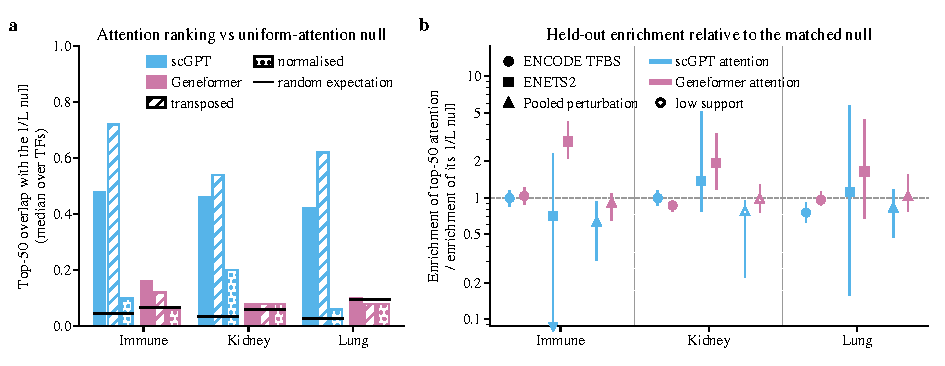
\includegraphics[width=\textwidth]{figS6_fm_attention_null.pdf}
  \caption{\textbf{Foundation-model attention against its uniform-attention null.} (a) Median over TFs of the overlap between the 50 top-ranked targets by attention and by the $1/L$ null (the attention an edge would receive if each cell spread attention uniformly over its $L$ input genes); filled: raw attention, hatched: transposed and normalised variants; black ticks: overlap expected for a random ranking. The 50 top targets of raw scGPT attention overlap with those of its null by 0.42--0.48 (random ranking 0.03--0.05), those of raw Geneformer attention by 0.08--0.16. (b) TF-matched held-out enrichment of each model's top-50-per-TF predicted set divided by that of its own $1/L$ null, with paired 95\% TF-cluster bootstrap intervals (reference line at 1; triangles mark lower limits below the axis range; open markers: references flagged as low support).}
  \label{fig:S-fm-null}
\end{figure}


\clearpage
\section{Informative-observation extension}\label{sec:S-obs}
Fits, cross-validation and held-out evaluation of the post hoc selection-model extension of Section~\ref{sec:obsmodel} (Section~\ref{sec:res-obs}).
% provenance: paper/r2/tables/tabS_obs_fit.tex generated by src/r2/paper_assets on 2026-10-15 04:06 from data/r2/tables/
%   obs_fit_summary.csv (modified 2026-10-14 20:37): all rows
\begin{table}[htbp]
\centering
\small
\setlength{\tabcolsep}{2.2pt}
\caption{Informative-observation extension (posterior mode, Laplace intervals) against the ignorable models: class weight of T, share of the joint log-likelihood due to observation, size of the BFDR\,$\le$\,0.05 set, mean credibility by evidence status, literature annotators whose observation rate is higher under T, and agreement with the ignorable counterpart.}
\label{tab:S-obs-fit}
\begin{tabular}{@{}lccrccccrl@{}}
\toprule
 & & Obs. & BFDR & \multicolumn{3}{c}{Mean credibility} & $\eta_{\mathrm T}>$ & & Alt. \\
\cmidrule(lr){5-7}
Fit & $w_{\mathrm T}$ & share & set $n$ & unobs. & obs.\,neg. & reported & $\eta_{\bar{\mathrm T}}$ & Spearman & optimum \\
\midrule
\multicolumn{10}{@{}l}{\emph{Global universe}} \\
Family-HB & 0.0031 & -- & 4{,}064 & 0.0031 & 0.0012 & 0.22 & -- & -- & -- \\
\quad + observation$^{\dagger}$ & \begin{tabular}[t]{@{}c@{}}0.68\\[-1pt]{\scriptsize [0.68, 0.68]}\end{tabular} & 0.98 & 6{,}096{,}120 & 0.97 & 0.44 & 0.20 & 0/18 & 0.67 & swapped \\
\quad + obs., TF-w.$^{\dagger}$ & \begin{tabular}[t]{@{}c@{}}0.0031\\[-1pt]{\scriptsize [0.0030, 0.0033]}\end{tabular} & 0.98 & 4{,}211 & 0.0031 & 0.0012 & 0.23 & 17/18 & 0.98 & 2nd optimum \\
EM baseline & 0.0068 & -- & 18{,}873 & 0.0068 & 0.0021 & 0.56 & -- & -- & -- \\
\quad + observation$^{\dagger}$ & \begin{tabular}[t]{@{}c@{}}0.32\\[-1pt]{\scriptsize [0.32, 0.32]}\end{tabular} & 0.98 & 2{,}275{,}210 & 0.033 & 0.56 & 0.81 & 18/18 & $-$0.82 & swapped \\
\quad + obs., TF-w.$^{\dagger}$ & \begin{tabular}[t]{@{}c@{}}0.0068\\[-1pt]{\scriptsize [0.0067, 0.0070]}\end{tabular} & 0.98 & 18{,}971 & 0.0068 & 0.0021 & 0.56 & 18/18 & 0.98 & none \\
\addlinespace[3pt]
\multicolumn{10}{@{}l}{\emph{Immune universe}} \\
Family-HB & 0.0063 & -- & 331 & 0.0063 & 0.0019 & 0.26 & -- & -- & -- \\
\quad + observation$^{\dagger}$ & \begin{tabular}[t]{@{}c@{}}0.65\\[-1pt]{\scriptsize [0.65, 0.65]}\end{tabular} & 0.97 & 169{,}386 & 0.89 & 0.30 & 0.064 & 0/18 & 0.76 & swapped \\
\quad + obs., TF-w.$^{\dagger}$ & \begin{tabular}[t]{@{}c@{}}0.0091\\[-1pt]{\scriptsize [0.0078, 0.011]}\end{tabular} & 0.97 & 514 & 0.0089 & 0.0016 & 0.44 & 18/18 & 0.77 & 2nd optimum \\
EM baseline & 0.015 & -- & 1{,}281 & 0.015 & 0.0040 & 0.65 & -- & -- & -- \\
\quad + observation$^{\dagger}$ & \begin{tabular}[t]{@{}c@{}}0.35\\[-1pt]{\scriptsize [0.35, 0.35]}\end{tabular} & 0.96 & 89{,}098 & 0.11 & 0.70 & 0.94 & 18/18 & $-$0.81 & swapped \\
\quad + obs., TF-w.$^{\dagger}$ & \begin{tabular}[t]{@{}c@{}}0.015\\[-1pt]{\scriptsize [0.014, 0.016]}\end{tabular} & 0.97 & 1{,}283 & 0.014 & 0.0038 & 0.65 & 18/18 & 1.00 & none \\
\addlinespace[3pt]
\multicolumn{10}{@{}l}{\emph{Kidney universe}} \\
Family-HB & 0.0063 & -- & 189 & 0.0063 & 0.0018 & 0.25 & -- & -- & -- \\
\quad + observation$^{\dagger}$ & \begin{tabular}[t]{@{}c@{}}0.68\\[-1pt]{\scriptsize [0.68, 0.68]}\end{tabular} & 0.97 & 111{,}065 & 0.92 & 0.34 & 0.079 & 0/18 & 0.78 & swapped \\
\quad + obs., TF-w.$^{\dagger}$ & \begin{tabular}[t]{@{}c@{}}0.012\\[-1pt]{\scriptsize [0.0098, 0.014]}\end{tabular} & 0.97 & 481 & 0.011 & 0.0027 & 0.53 & 18/18 & 0.83 & 2nd optimum \\
EM baseline & 0.016 & -- & 812 & 0.016 & 0.0043 & 0.65 & -- & -- & -- \\
\quad + observation$^{\dagger}$ & \begin{tabular}[t]{@{}c@{}}0.32\\[-1pt]{\scriptsize [0.31, 0.32]}\end{tabular} & 0.96 & 49{,}909 & 0.075 & 0.65 & 0.93 & 18/18 & $-$0.82 & swapped \\
\quad + obs., TF-w.$^{\dagger}$ & \begin{tabular}[t]{@{}c@{}}0.015\\[-1pt]{\scriptsize [0.014, 0.017]}\end{tabular} & 0.97 & 820 & 0.015 & 0.0040 & 0.66 & 18/18 & 0.99 & none \\
\addlinespace[3pt]
\multicolumn{10}{@{}l}{\emph{Lung universe}} \\
Family-HB & 0.0047 & -- & 245 & 0.0047 & 0.0011 & 0.25 & -- & -- & -- \\
\quad + observation$^{\dagger}$ & \begin{tabular}[t]{@{}c@{}}0.63\\[-1pt]{\scriptsize [0.63, 0.63]}\end{tabular} & 0.98 & 189{,}960 & 0.92 & 0.27 & 0.069 & 0/18 & 0.85 & swapped \\
\quad + obs., TF-w.$^{\dagger}$ & \begin{tabular}[t]{@{}c@{}}0.0073\\[-1pt]{\scriptsize [0.0063, 0.0086]}\end{tabular} & 0.98 & 412 & 0.0072 & 0.0013 & 0.43 & 18/18 & 0.87 & 2nd optimum \\
EM baseline & 0.012 & -- & 1{,}230 & 0.012 & 0.0025 & 0.63 & -- & -- & -- \\
\quad + observation$^{\dagger}$ & \begin{tabular}[t]{@{}c@{}}0.37\\[-1pt]{\scriptsize [0.37, 0.37]}\end{tabular} & 0.97 & 113{,}129 & 0.078 & 0.73 & 0.93 & 17/18 & $-$0.87 & swapped \\
\quad + obs., TF-w.$^{\dagger}$ & \begin{tabular}[t]{@{}c@{}}0.011\\[-1pt]{\scriptsize [0.010, 0.012]}\end{tabular} & 0.98 & 1{,}231 & 0.011 & 0.0024 & 0.63 & 17/18 & 1.00 & none \\
\bottomrule
\end{tabular}
\par\smallskip
\begin{minipage}{\linewidth}\footnotesize
Obs.\ share: observation term over the joint log-likelihood. $\eta_{\mathrm T}>\eta_{\bar{\mathrm T}}$: literature annotators that observe true edges more often than non-edges. Spearman: credibility of observed edges against the ignorable counterpart. Alt.\ optimum: role of the next optimum (label-swapped: T and burst classes exchanged).

$^{\dagger}$\,Post hoc: defined after the held-out data had been examined.
\end{minipage}
\end{table}

% provenance: paper/r2/tables/tabS_obs_cv.tex generated by src/r2/paper_assets on 2026-10-15 04:06 from data/r2/tables/
%   obs_cv.csv (modified 2026-10-14 20:37): all rows
\begin{table}[htbp]
\centering
\small
\caption{Cross-validated held-out log-likelihood (5 folds by TF) of the informative-observation models and their ignorable counterparts: of the reports given the observation pattern (per observed edge), of the observation indicators and of both (per edge).}
\label{tab:S-obs-cv}
\begin{tabular}{@{}lccc@{}}
\toprule
Model & Reports $|$ observation & Observation & Joint \\
\midrule
\multicolumn{4}{@{}l}{\emph{Global universe}} \\
Family-HB & $-$0.0681 & $-$2.4537$^{\dagger}$ & $-$2.4909$^{\dagger}$ \\
Family-HB + obs. & $-$0.0684 ($-2.7\times 10^{-4}$)$^{\dagger}$ & $-$2.0539 (0.40)$^{\dagger}$ & $-$2.0913 (0.40)$^{\dagger}$ \\
Family-HB + obs., TF-weighted & $-$0.0681 ($1.6\times 10^{-5}$)$^{\dagger}$ & $-$2.4499 (0.0039)$^{\dagger}$ & $-$2.4883 (0.0026)$^{\dagger}$ \\
EM baseline & $-$0.0687 & $-$2.4537$^{\dagger}$ & $-$2.4912$^{\dagger}$ \\
EM + obs. & $-$0.0847 ($-$0.016)$^{\dagger}$ & $-$2.0539 (0.40)$^{\dagger}$ & $-$2.1002 (0.39)$^{\dagger}$ \\
EM + obs., TF-weighted & $-$0.0687 ($4.5\times 10^{-5}$)$^{\dagger}$ & $-$2.4421 (0.012)$^{\dagger}$ & $-$2.4849 (0.0064)$^{\dagger}$ \\
\addlinespace[3pt]
\multicolumn{4}{@{}l}{\emph{Immune universe}} \\
Family-HB & $-$0.1395 & $-$2.5555$^{\dagger}$ & $-$2.6111$^{\dagger}$ \\
Family-HB + obs. & $-$0.1405 ($-1.0\times 10^{-3}$)$^{\dagger}$ & $-$1.9097 (0.65)$^{\dagger}$ & $-$1.9657 (0.65)$^{\dagger}$ \\
Family-HB + obs., TF-weighted & $-$0.1392 ($3.0\times 10^{-4}$)$^{\dagger}$ & $-$2.5312 (0.024)$^{\dagger}$ & $-$2.6002 (0.011)$^{\dagger}$ \\
EM baseline & $-$0.1414 & $-$2.5555$^{\dagger}$ & $-$2.6118$^{\dagger}$ \\
EM + obs. & $-$0.1812 ($-$0.040)$^{\dagger}$ & $-$1.9097 (0.65)$^{\dagger}$ & $-$1.9819 (0.63)$^{\dagger}$ \\
EM + obs., TF-weighted & $-$0.1407 ($6.8\times 10^{-4}$)$^{\dagger}$ & $-$2.5220 (0.033)$^{\dagger}$ & $-$2.5957 (0.016)$^{\dagger}$ \\
\bottomrule
\end{tabular}
\par\smallskip
\begin{minipage}{\linewidth}\footnotesize
In parentheses: difference to the ignorable counterpart (Family-HB or EM) on the same folds. For the ignorable models the observation term is a class-independent Bernoulli model of the literature observation indicators.

$^{\dagger}$\,Post hoc: defined after the held-out data had been examined.
\end{minipage}
\end{table}

% provenance: paper/r2/tables/tabS_obs_heldout.tex generated by src/r2/paper_assets on 2026-10-15 04:06 from data/r2/tables/
%   obs_heldout.csv (modified 2026-10-14 20:37): universe == global
\begin{table}[htbp]
\centering
\small
\caption{Held-out evaluation of the informative-observation extension in the global universe (all evaluable edges): AP lift [95\% TF-cluster bootstrap interval], within-TF AUROC and stratified Enr@500, with the primary estimators, Fisher, the post hoc status scores and random.}
\label{tab:S-obs-heldout}
\begin{tabular}{@{}lccc@{}}
\toprule
Score & AP lift [95\% CI] & Within-TF AUROC & Strat.\ Enr@500 \\
\midrule
\multicolumn{4}{@{}l}{\emph{ENCODE TFBS}} \\
Family-HB + obs.$^{\dagger}$ & 0.97 [0.94, 0.99] & 0.483 & 1.11 \\
EM + obs.$^{\dagger}$ & 1.02 [1.01, 1.03] & 0.517 & 1.07 \\
Family-HB + obs., TF-weighted$^{\dagger}$ & 0.97 [0.94, 1.02] & 0.481 & 1.32 \\
EM + obs., TF-weighted$^{\dagger}$ & 0.98 [0.95, 1.02] & 0.489 & 1.33 \\
Family-HB + obs., swapped labels$^{\dagger}$ & 1.02 [1.01, 1.02] & 0.516 & 1.05 \\
EM + obs., swapped labels$^{\dagger}$ & 0.97 [0.94, 0.99] & 0.484 & 1.11 \\
Family-HB & 0.96 [0.94, 0.98] & 0.481 & 1.32 \\
EM baseline & 0.96 [0.95, 0.98] & 0.489 & 1.33 \\
Fisher & 1.07 [1.05, 1.08] & 0.547 & 1.50 \\
3-level status$^{\dagger}$ & 1.05 [1.03, 1.07] & 0.537 & 1.13 \\
Family-HB, unobserved last$^{\dagger}$ & 1.07 [1.05, 1.10] & 0.545 & 1.32 \\
Random & 1.00 [1.00, 1.00] & 0.500 & 1.01 \\
\addlinespace[3pt]
\multicolumn{4}{@{}l}{\emph{ENETS2}} \\
Family-HB + obs.$^{\dagger}$ & 0.95 [0.91, 1.00] & 0.474 & 1.31 \\
EM + obs.$^{\dagger}$ & 1.22 [1.13, 1.34] & 0.525 & 1.53 \\
Family-HB + obs., TF-weighted$^{\dagger}$ & 1.75 [1.42, 2.19] & 0.522 & 6.97 \\
EM + obs., TF-weighted$^{\dagger}$ & 1.65 [1.38, 2.02] & 0.529 & 7.07 \\
Family-HB + obs., swapped labels$^{\dagger}$ & 1.14 [1.06, 1.22] & 0.518 & 1.05 \\
EM + obs., swapped labels$^{\dagger}$ & 0.95 [0.92, 1.00] & 0.477 & 1.31 \\
Family-HB & 1.59 [1.31, 2.00] & 0.522 & 6.79 \\
EM baseline & 1.49 [1.26, 1.83] & 0.529 & 7.09 \\
Fisher & 1.80 [1.48, 2.27] & 0.537 & 9.34 \\
3-level status$^{\dagger}$ & 1.38 [1.24, 1.59] & 0.540 & 2.82 \\
Family-HB, unobserved last$^{\dagger}$ & 1.79 [1.46, 2.25] & 0.537 & 6.79 \\
Random & 1.01 [0.99, 1.03] & 0.503 & 1.11 \\
\addlinespace[3pt]
\multicolumn{4}{@{}l}{\emph{Pooled perturbation}} \\
Family-HB + obs.$^{\dagger}$ & 1.10 [0.99, 1.24] & 0.463 & 0.99 \\
EM + obs.$^{\dagger}$ & 1.13 [1.10, 1.18] & 0.536 & 0.98 \\
Family-HB + obs., TF-weighted$^{\dagger}$ & 0.93 [0.86, 1.05] & 0.478 & 1.55 \\
EM + obs., TF-weighted$^{\dagger}$ & 0.94 [0.87, 1.04] & 0.479 & 1.46 \\
Family-HB + obs., swapped labels$^{\dagger}$ & 1.12 [1.09, 1.17] & 0.532 & 1.01 \\
EM + obs., swapped labels$^{\dagger}$ & 1.10 [0.99, 1.24] & 0.464 & 0.99 \\
Family-HB & 0.94 [0.90, 0.98] & 0.478 & 1.53 \\
EM baseline & 0.94 [0.90, 0.98] & 0.479 & 1.47 \\
Fisher & 1.01 [0.98, 1.06] & 0.497 & 1.52 \\
3-level status$^{\dagger}$ & 1.06 [1.02, 1.12] & 0.519 & 1.25 \\
Family-HB, unobserved last$^{\dagger}$ & 1.03 [0.99, 1.09] & 0.501 & 1.53 \\
Random & 0.99 [0.99, 1.00] & 0.508 & 0.85 \\
\bottomrule
\end{tabular}
\par\smallskip
\begin{minipage}{\linewidth}\footnotesize
$^{\dagger}$\,Post hoc: defined after the held-out data had been examined.
\end{minipage}
\end{table}

% generated by src/r2/paper_assets (make_paper_assets.py figures); do not edit by hand
% provenance: figS2_obs_model generated by src/r2/paper_assets on 2026-10-15 04:07 from data/r2/tables/
%   obs_params.csv (modified 2026-10-14 20:37): universe == 'global', optimum_role == 'best', fit_id in (family_hb_obs, em_obs), observation_modelled == True
%   obs_fit_summary.csv (modified 2026-10-14 20:37): fit_id in (family_hb, em, family_hb_obs, em_obs); all universes; columns mean_cred_unobserved / _observed_neg / _reported
\begin{figure}[htbp]
  \centering
  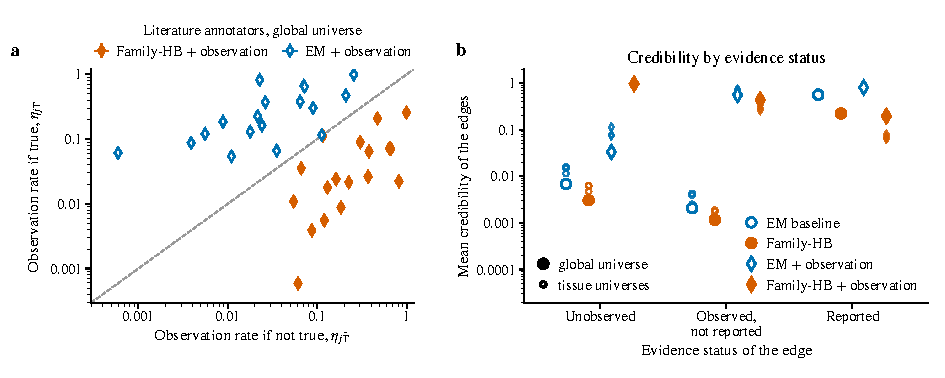
\includegraphics[width=\textwidth]{figS2_obs_model.pdf}
  \caption{\textbf{Informative-observation extension} (secondary, post hoc; MAP fits with Laplace 95\% intervals). (a) Observation rates of the 18 literature annotators under the true class and under the other classes at the best optimum of Family-HB + observation and EM + observation (global universe; dashed: equal rates, i.e. ignorable observation). The two models place most of their annotators on opposite sides of the diagonal (above it: 0 of 18 for Family-HB + observation, 18 of 18 for EM + observation): the label T is not anchored. (b) Mean credibility of unobserved, observed-but-unreported and reported edges for the ignorable models (EM, Family-HB) and the extensions (large markers: global universe; small open markers: immune, kidney and lung). In the global universe Family-HB + observation gives unobserved edges the highest mean credibility (0.97); EM + observation ranks them below observed-but-unreported edges (0.033 vs 0.56).}
  \label{fig:S-obs}
\end{figure}


\clearpage
\section{Claim governance}\label{sec:S-gov}
Sensitivity of the promoted set and of its held-out enrichment to the BFDR thresholds and to the tier rules, and the label-free deconcentration of the promoted set (Sections~\ref{sec:governance} and \ref{sec:res-governance}).
% provenance: paper/r2/tables/tabS_gov_grid.tex generated by src/r2/paper_assets on 2026-10-15 04:06 from data/r2/tables/
%   gov_sensitivity_grid.csv (modified 2026-10-14 20:11): reference == encode; q_grid rows with q_strong == primary q_strong
\begin{table}[htbp]
\centering
\small
\setlength{\tabcolsep}{3pt}
\caption{Sensitivity of the promoted set to the governance rules: size, Jaccard index with the primary promoted set, and TF-matched held-out O/E (ENCODE TFBS, 95\% TF-cluster bootstrap interval).}
\label{tab:S-gov-grid}
\begin{tabular}{@{}lrccrccrcc@{}}
\toprule
 & \multicolumn{3}{c}{Immune} & \multicolumn{3}{c}{Kidney} & \multicolumn{3}{c}{Lung} \\
\cmidrule(lr){2-4}\cmidrule(lr){5-7}\cmidrule(lr){8-10}
Rule & $n$ & Jaccard & O/E & $n$ & Jaccard & O/E & $n$ & Jaccard & O/E \\
\midrule
\multicolumn{10}{@{}l}{\emph{Threshold grid}} \\
$q_M$ = 0.10 & 363 & 0.74 & \begin{tabular}[t]{@{}c@{}}1.63\\[-1pt]{\scriptsize [1.27, 2.31]}\end{tabular} & 188 & 0.68 & \begin{tabular}[t]{@{}c@{}}1.24\\[-1pt]{\scriptsize [1.04, 1.72]}\end{tabular} & 282 & 0.68 & \begin{tabular}[t]{@{}c@{}}2.23\\[-1pt]{\scriptsize [1.76, 3.03]}\end{tabular} \\
$q_M$ = 0.20 & 493 & 1.00 & \begin{tabular}[t]{@{}c@{}}1.67\\[-1pt]{\scriptsize [1.35, 2.38]}\end{tabular} & 276 & 1.00 & \begin{tabular}[t]{@{}c@{}}1.24\\[-1pt]{\scriptsize [1.03, 1.81]}\end{tabular} & 412 & 1.00 & \begin{tabular}[t]{@{}c@{}}2.27\\[-1pt]{\scriptsize [1.78, 3.37]}\end{tabular} \\
$q_M$ = 0.30 & 596 & 0.83 & \begin{tabular}[t]{@{}c@{}}1.66\\[-1pt]{\scriptsize [1.40, 2.35]}\end{tabular} & 350 & 0.79 & \begin{tabular}[t]{@{}c@{}}1.22\\[-1pt]{\scriptsize [1.04, 1.81]}\end{tabular} & 538 & 0.77 & \begin{tabular}[t]{@{}c@{}}2.16\\[-1pt]{\scriptsize [1.68, 3.02]}\end{tabular} \\
$q_M$ = 0.40 & 755 & 0.65 & \begin{tabular}[t]{@{}c@{}}1.58\\[-1pt]{\scriptsize [1.36, 2.06]}\end{tabular} & 443 & 0.62 & \begin{tabular}[t]{@{}c@{}}1.18\\[-1pt]{\scriptsize [1.02, 1.64]}\end{tabular} & 666 & 0.62 & \begin{tabular}[t]{@{}c@{}}2.07\\[-1pt]{\scriptsize [1.71, 2.76]}\end{tabular} \\
\addlinespace[3pt]
\multicolumn{10}{@{}l}{\emph{Dual-universe rule}} \\
primary & 493 & 1.00 & \begin{tabular}[t]{@{}c@{}}1.67\\[-1pt]{\scriptsize [1.35, 2.38]}\end{tabular} & 276 & 1.00 & \begin{tabular}[t]{@{}c@{}}1.24\\[-1pt]{\scriptsize [1.03, 1.81]}\end{tabular} & 412 & 1.00 & \begin{tabular}[t]{@{}c@{}}2.27\\[-1pt]{\scriptsize [1.78, 3.37]}\end{tabular} \\
lenient (+1 tier) & 493 & 1.00 & \begin{tabular}[t]{@{}c@{}}1.67\\[-1pt]{\scriptsize [1.35, 2.38]}\end{tabular} & 276 & 1.00 & \begin{tabular}[t]{@{}c@{}}1.24\\[-1pt]{\scriptsize [1.03, 1.81]}\end{tabular} & 412 & 1.00 & \begin{tabular}[t]{@{}c@{}}2.27\\[-1pt]{\scriptsize [1.78, 3.37]}\end{tabular} \\
strict ($-$1 tier) & 341 & 0.69 & \begin{tabular}[t]{@{}c@{}}1.59\\[-1pt]{\scriptsize [1.26, 2.26]}\end{tabular} & 186 & 0.67 & \begin{tabular}[t]{@{}c@{}}1.24\\[-1pt]{\scriptsize [1.04, 1.69]}\end{tabular} & 248 & 0.60 & \begin{tabular}[t]{@{}c@{}}2.21\\[-1pt]{\scriptsize [1.75, 3.19]}\end{tabular} \\
\addlinespace[3pt]
\multicolumn{10}{@{}l}{\emph{Single fit}} \\
global fit only & 506 & 0.97 & \begin{tabular}[t]{@{}c@{}}1.64\\[-1pt]{\scriptsize [1.35, 2.28]}\end{tabular} & 282 & 0.98 & \begin{tabular}[t]{@{}c@{}}1.20\\[-1pt]{\scriptsize [1.01, 1.76]}\end{tabular} & 423 & 0.97 & \begin{tabular}[t]{@{}c@{}}2.22\\[-1pt]{\scriptsize [1.77, 3.12]}\end{tabular} \\
global fit, Strong only & 304 & 0.62 & \begin{tabular}[t]{@{}c@{}}1.62\\[-1pt]{\scriptsize [1.28, 2.22]}\end{tabular} & 156 & 0.57 & \begin{tabular}[t]{@{}c@{}}1.22\\[-1pt]{\scriptsize [1.03, 1.74]}\end{tabular} & 220 & 0.53 & \begin{tabular}[t]{@{}c@{}}2.16\\[-1pt]{\scriptsize [1.74, 2.94]}\end{tabular} \\
context fit only & 553 & 0.89 & \begin{tabular}[t]{@{}c@{}}1.65\\[-1pt]{\scriptsize [1.36, 2.31]}\end{tabular} & 326 & 0.85 & \begin{tabular}[t]{@{}c@{}}1.24\\[-1pt]{\scriptsize [1.04, 1.76]}\end{tabular} & 464 & 0.89 & \begin{tabular}[t]{@{}c@{}}2.31\\[-1pt]{\scriptsize [1.83, 3.41]}\end{tabular} \\
context fit, Strong only & 334 & 0.68 & \begin{tabular}[t]{@{}c@{}}1.59\\[-1pt]{\scriptsize [1.26, 2.22]}\end{tabular} & 179 & 0.65 & \begin{tabular}[t]{@{}c@{}}1.27\\[-1pt]{\scriptsize [1.08, 1.82]}\end{tabular} & 232 & 0.56 & \begin{tabular}[t]{@{}c@{}}2.27\\[-1pt]{\scriptsize [1.70, 3.36]}\end{tabular} \\
\addlinespace[3pt]
\multicolumn{10}{@{}l}{\emph{Rank budget}} \\
rank budget & 2{,}008 & 0.25 & \begin{tabular}[t]{@{}c@{}}1.42\\[-1pt]{\scriptsize [1.27, 1.77]}\end{tabular} & -- & -- & -- & -- & -- & -- \\
\addlinespace[3pt]
\multicolumn{10}{@{}l}{\emph{Credibility}} \\
NUTS mean (primary) & 493 & 1.00 & \begin{tabular}[t]{@{}c@{}}1.67\\[-1pt]{\scriptsize [1.35, 2.38]}\end{tabular} & 276 & 1.00 & \begin{tabular}[t]{@{}c@{}}1.24\\[-1pt]{\scriptsize [1.03, 1.81]}\end{tabular} & 412 & 1.00 & \begin{tabular}[t]{@{}c@{}}2.27\\[-1pt]{\scriptsize [1.78, 3.37]}\end{tabular} \\
posterior mode & 484 & 0.98 & \begin{tabular}[t]{@{}c@{}}1.66\\[-1pt]{\scriptsize [1.36, 2.33]}\end{tabular} & 274 & 0.97 & \begin{tabular}[t]{@{}c@{}}1.23\\[-1pt]{\scriptsize [1.04, 1.81]}\end{tabular} & 409 & 0.99 & \begin{tabular}[t]{@{}c@{}}2.28\\[-1pt]{\scriptsize [1.79, 3.32]}\end{tabular} \\
\addlinespace[3pt]
\multicolumn{10}{@{}l}{\emph{Estimator}} \\
EM baseline & 1{,}659 & 0.30 & \begin{tabular}[t]{@{}c@{}}1.45\\[-1pt]{\scriptsize [1.29, 1.82]}\end{tabular} & 1{,}051 & 0.26 & \begin{tabular}[t]{@{}c@{}}1.12\\[-1pt]{\scriptsize [1.00, 1.33]}\end{tabular} & 1{,}608 & 0.26 & \begin{tabular}[t]{@{}c@{}}1.71\\[-1pt]{\scriptsize [1.52, 2.11]}\end{tabular} \\
\bottomrule
\end{tabular}
\end{table}

\begin{table}[htbp]
\ContinuedFloat
\centering
\small
\setlength{\tabcolsep}{3pt}
\caption{Sensitivity of the promoted set to the governance rules: size, Jaccard index with the primary promoted set, and TF-matched held-out O/E (ENCODE TFBS, 95\% TF-cluster bootstrap interval). (continued)}
\label{tab:S-gov-grid-b}
\begin{tabular}{@{}lrccrccrcc@{}}
\toprule
 & \multicolumn{3}{c}{Immune} & \multicolumn{3}{c}{Kidney} & \multicolumn{3}{c}{Lung} \\
\cmidrule(lr){2-4}\cmidrule(lr){5-7}\cmidrule(lr){8-10}
Rule & $n$ & Jaccard & O/E & $n$ & Jaccard & O/E & $n$ & Jaccard & O/E \\
\midrule
\multicolumn{10}{@{}l}{\emph{Simple rules}} \\
majority ($\geq$2 reports) & 1{,}102 & 0.40 & \begin{tabular}[t]{@{}c@{}}1.62\\[-1pt]{\scriptsize [1.41, 2.10]}\end{tabular} & 720 & 0.36 & \begin{tabular}[t]{@{}c@{}}1.16\\[-1pt]{\scriptsize [1.02, 1.45]}\end{tabular} & 1{,}079 & 0.35 & \begin{tabular}[t]{@{}c@{}}1.84\\[-1pt]{\scriptsize [1.54, 2.41]}\end{tabular} \\
union ($\geq$1 report) & 2{,}216 & 0.22 & \begin{tabular}[t]{@{}c@{}}1.44\\[-1pt]{\scriptsize [1.28, 1.78]}\end{tabular} & 1{,}439 & 0.19 & \begin{tabular}[t]{@{}c@{}}1.09\\[-1pt]{\scriptsize [0.99, 1.28]}\end{tabular} & 2{,}178 & 0.19 & \begin{tabular}[t]{@{}c@{}}1.65\\[-1pt]{\scriptsize [1.51, 2.08]}\end{tabular} \\
DoRothEA A/B & 269 & 0.50 & \begin{tabular}[t]{@{}c@{}}1.67\\[-1pt]{\scriptsize [1.44, 2.15]}\end{tabular} & 165 & 0.52 & \begin{tabular}[t]{@{}c@{}}1.16\\[-1pt]{\scriptsize [0.98, 1.69]}\end{tabular} & 181 & 0.39 & \begin{tabular}[t]{@{}c@{}}2.04\\[-1pt]{\scriptsize [1.46, 3.13]}\end{tabular} \\
CollecTRI member & 2{,}041 & 0.24 & \begin{tabular}[t]{@{}c@{}}1.44\\[-1pt]{\scriptsize [1.26, 1.81]}\end{tabular} & 1{,}289 & 0.21 & \begin{tabular}[t]{@{}c@{}}1.11\\[-1pt]{\scriptsize [1.00, 1.27]}\end{tabular} & 2{,}022 & 0.20 & \begin{tabular}[t]{@{}c@{}}1.67\\[-1pt]{\scriptsize [1.51, 2.01]}\end{tabular} \\
\addlinespace[3pt]
\multicolumn{10}{@{}l}{\emph{Size-matched to primary}} \\
joint, NUTS$^{\dagger}$ & 493 & 1.00 & \begin{tabular}[t]{@{}c@{}}1.68\\[-1pt]{\scriptsize [1.35, 2.36]}\end{tabular} & -- & -- & -- & -- & -- & -- \\
joint, mode$^{\dagger}$ & 493 & 0.96 & \begin{tabular}[t]{@{}c@{}}1.69\\[-1pt]{\scriptsize [1.36, 2.41]}\end{tabular} & -- & -- & -- & -- & -- & -- \\
joint, EM$^{\dagger}$ & 493 & 0.35 & \begin{tabular}[t]{@{}c@{}}1.77\\[-1pt]{\scriptsize [1.50, 2.44]}\end{tabular} & -- & -- & -- & -- & -- & -- \\
global fit, NUTS$^{\dagger}$ & 493 & 0.96 & \begin{tabular}[t]{@{}c@{}}1.63\\[-1pt]{\scriptsize [1.31, 2.34]}\end{tabular} & -- & -- & -- & -- & -- & -- \\
context fit, NUTS$^{\dagger}$ & 493 & 0.92 & \begin{tabular}[t]{@{}c@{}}1.68\\[-1pt]{\scriptsize [1.39, 2.36]}\end{tabular} & -- & -- & -- & -- & -- & -- \\
number of reports$^{\dagger}$ & 493 & 0.48 & \begin{tabular}[t]{@{}c@{}}1.75\\[-1pt]{\scriptsize [1.48, 2.24]}\end{tabular} & -- & -- & -- & -- & -- & -- \\
DoRothEA level$^{\dagger}$ & 493 & 0.48 & \begin{tabular}[t]{@{}c@{}}1.69\\[-1pt]{\scriptsize [1.46, 2.29]}\end{tabular} & -- & -- & -- & -- & -- & -- \\
CollecTRI effort$^{\dagger}$ & 493 & 0.13 & \begin{tabular}[t]{@{}c@{}}1.39\\[-1pt]{\scriptsize [1.18, 1.84]}\end{tabular} & -- & -- & -- & -- & -- & -- \\
\bottomrule
\end{tabular}
\par\smallskip
\begin{minipage}{\linewidth}\footnotesize
Threshold grid: moderate threshold $q_M$ at the primary strong threshold $q_S$ = 0.05 (the promoted set does not depend on $q_S$). $^{*}$\,Few TF clusters.

$^{\dagger}$\,Post hoc: defined after the held-out data had been examined.
\end{minipage}
\end{table}

% provenance: paper/r2/tables/tabS_gov_grid_pert.tex generated by src/r2/paper_assets on 2026-10-15 04:06 from data/r2/tables/
%   gov_sensitivity_grid.csv (modified 2026-10-14 20:11): reference == pert_pooled; q_grid rows with q_strong == primary q_strong
\begin{table}[htbp]
\centering
\small
\setlength{\tabcolsep}{3pt}
\caption{Sensitivity of the promoted set to the governance rules: size, Jaccard index with the primary promoted set, and TF-matched held-out O/E (Pooled perturbation, 95\% TF-cluster bootstrap interval).}
\label{tab:S-gov-grid-pert}
\begin{tabular}{@{}lrccrccrcc@{}}
\toprule
 & \multicolumn{3}{c}{Immune} & \multicolumn{3}{c}{Kidney} & \multicolumn{3}{c}{Lung} \\
\cmidrule(lr){2-4}\cmidrule(lr){5-7}\cmidrule(lr){8-10}
Rule & $n$ & Jaccard & O/E & $n$ & Jaccard & O/E & $n$ & Jaccard & O/E \\
\midrule
\multicolumn{10}{@{}l}{\emph{Threshold grid}} \\
$q_M$ = 0.10 & 363 & 0.74 & \begin{tabular}[t]{@{}c@{}}1.23$^{*}$\\[-1pt]{\scriptsize [0.69, 1.88]}\end{tabular} & 188 & 0.68 & \begin{tabular}[t]{@{}c@{}}0.98$^{*}$\\[-1pt]{\scriptsize [0.70, 1.60]}\end{tabular} & 282 & 0.68 & \begin{tabular}[t]{@{}c@{}}1.26$^{*}$\\[-1pt]{\scriptsize [1.12, 1.44]}\end{tabular} \\
$q_M$ = 0.20 & 493 & 1.00 & \begin{tabular}[t]{@{}c@{}}1.20\\[-1pt]{\scriptsize [0.82, 1.64]}\end{tabular} & 276 & 1.00 & \begin{tabular}[t]{@{}c@{}}0.66$^{*}$\\[-1pt]{\scriptsize [0.00, 1.00]}\end{tabular} & 412 & 1.00 & \begin{tabular}[t]{@{}c@{}}1.29$^{*}$\\[-1pt]{\scriptsize [1.13, 1.57]}\end{tabular} \\
$q_M$ = 0.30 & 596 & 0.83 & \begin{tabular}[t]{@{}c@{}}1.18\\[-1pt]{\scriptsize [0.86, 1.58]}\end{tabular} & 350 & 0.79 & \begin{tabular}[t]{@{}c@{}}0.77$^{*}$\\[-1pt]{\scriptsize [0.00, 0.94]}\end{tabular} & 538 & 0.77 & \begin{tabular}[t]{@{}c@{}}1.24$^{*}$\\[-1pt]{\scriptsize [1.08, 1.44]}\end{tabular} \\
$q_M$ = 0.40 & 755 & 0.65 & \begin{tabular}[t]{@{}c@{}}1.21\\[-1pt]{\scriptsize [0.86, 1.77]}\end{tabular} & 443 & 0.62 & \begin{tabular}[t]{@{}c@{}}0.85$^{*}$\\[-1pt]{\scriptsize [0.00, 1.34]}\end{tabular} & 666 & 0.62 & \begin{tabular}[t]{@{}c@{}}1.20$^{*}$\\[-1pt]{\scriptsize [0.86, 1.49]}\end{tabular} \\
\addlinespace[3pt]
\multicolumn{10}{@{}l}{\emph{Dual-universe rule}} \\
primary & 493 & 1.00 & \begin{tabular}[t]{@{}c@{}}1.20\\[-1pt]{\scriptsize [0.82, 1.64]}\end{tabular} & 276 & 1.00 & \begin{tabular}[t]{@{}c@{}}0.66$^{*}$\\[-1pt]{\scriptsize [0.00, 1.00]}\end{tabular} & 412 & 1.00 & \begin{tabular}[t]{@{}c@{}}1.29$^{*}$\\[-1pt]{\scriptsize [1.13, 1.57]}\end{tabular} \\
lenient (+1 tier) & 493 & 1.00 & \begin{tabular}[t]{@{}c@{}}1.20\\[-1pt]{\scriptsize [0.82, 1.64]}\end{tabular} & 276 & 1.00 & \begin{tabular}[t]{@{}c@{}}0.66$^{*}$\\[-1pt]{\scriptsize [0.00, 1.00]}\end{tabular} & 412 & 1.00 & \begin{tabular}[t]{@{}c@{}}1.29$^{*}$\\[-1pt]{\scriptsize [1.13, 1.57]}\end{tabular} \\
strict ($-$1 tier) & 341 & 0.69 & \begin{tabular}[t]{@{}c@{}}1.18$^{*}$\\[-1pt]{\scriptsize [0.66, 1.81]}\end{tabular} & 186 & 0.67 & \begin{tabular}[t]{@{}c@{}}1.11$^{*}$\\[-1pt]{\scriptsize [0.84, 1.60]}\end{tabular} & 248 & 0.60 & \begin{tabular}[t]{@{}c@{}}1.14$^{*}$\\[-1pt]{\scriptsize [0.95, 1.44]}\end{tabular} \\
\addlinespace[3pt]
\multicolumn{10}{@{}l}{\emph{Single fit}} \\
global fit only & 506 & 0.97 & \begin{tabular}[t]{@{}c@{}}1.16\\[-1pt]{\scriptsize [0.80, 1.60]}\end{tabular} & 282 & 0.98 & \begin{tabular}[t]{@{}c@{}}0.66$^{*}$\\[-1pt]{\scriptsize [0.00, 1.00]}\end{tabular} & 423 & 0.97 & \begin{tabular}[t]{@{}c@{}}1.29$^{*}$\\[-1pt]{\scriptsize [1.13, 1.57]}\end{tabular} \\
global fit, Strong only & 304 & 0.62 & \begin{tabular}[t]{@{}c@{}}1.17$^{*}$\\[-1pt]{\scriptsize [0.68, 1.94]}\end{tabular} & 156 & 0.57 & \begin{tabular}[t]{@{}c@{}}1.51$^{*}$\\[-1pt]{\scriptsize [1.05, 2.67]}\end{tabular} & 220 & 0.53 & \begin{tabular}[t]{@{}c@{}}0.99$^{*}$\\[-1pt]{\scriptsize [0.81, 1.44]}\end{tabular} \\
context fit only & 553 & 0.89 & \begin{tabular}[t]{@{}c@{}}1.13\\[-1pt]{\scriptsize [0.72, 1.55]}\end{tabular} & 326 & 0.85 & \begin{tabular}[t]{@{}c@{}}0.61$^{*}$\\[-1pt]{\scriptsize [0.00, 0.80]}\end{tabular} & 464 & 0.89 & \begin{tabular}[t]{@{}c@{}}1.32$^{*}$\\[-1pt]{\scriptsize [1.18, 1.57]}\end{tabular} \\
context fit, Strong only & 334 & 0.68 & \begin{tabular}[t]{@{}c@{}}1.18$^{*}$\\[-1pt]{\scriptsize [0.66, 1.81]}\end{tabular} & 179 & 0.65 & \begin{tabular}[t]{@{}c@{}}1.11$^{*}$\\[-1pt]{\scriptsize [0.84, 1.60]}\end{tabular} & 232 & 0.56 & \begin{tabular}[t]{@{}c@{}}1.06$^{*}$\\[-1pt]{\scriptsize [0.81, 1.44]}\end{tabular} \\
\addlinespace[3pt]
\multicolumn{10}{@{}l}{\emph{Rank budget}} \\
rank budget & 2{,}008 & 0.25 & \begin{tabular}[t]{@{}c@{}}1.14\\[-1pt]{\scriptsize [0.96, 1.37]}\end{tabular} & -- & -- & -- & -- & -- & -- \\
\addlinespace[3pt]
\multicolumn{10}{@{}l}{\emph{Credibility}} \\
NUTS mean (primary) & 493 & 1.00 & \begin{tabular}[t]{@{}c@{}}1.20\\[-1pt]{\scriptsize [0.82, 1.64]}\end{tabular} & 276 & 1.00 & \begin{tabular}[t]{@{}c@{}}0.66$^{*}$\\[-1pt]{\scriptsize [0.00, 1.00]}\end{tabular} & 412 & 1.00 & \begin{tabular}[t]{@{}c@{}}1.29$^{*}$\\[-1pt]{\scriptsize [1.13, 1.57]}\end{tabular} \\
posterior mode & 484 & 0.98 & \begin{tabular}[t]{@{}c@{}}1.21\\[-1pt]{\scriptsize [0.85, 1.66]}\end{tabular} & 274 & 0.97 & \begin{tabular}[t]{@{}c@{}}0.66$^{*}$\\[-1pt]{\scriptsize [0.00, 1.00]}\end{tabular} & 409 & 0.99 & \begin{tabular}[t]{@{}c@{}}1.29$^{*}$\\[-1pt]{\scriptsize [1.13, 1.57]}\end{tabular} \\
\addlinespace[3pt]
\multicolumn{10}{@{}l}{\emph{Estimator}} \\
EM baseline & 1{,}659 & 0.30 & \begin{tabular}[t]{@{}c@{}}1.17\\[-1pt]{\scriptsize [0.98, 1.41]}\end{tabular} & 1{,}051 & 0.26 & \begin{tabular}[t]{@{}c@{}}1.01$^{*}$\\[-1pt]{\scriptsize [0.81, 2.41]}\end{tabular} & 1{,}608 & 0.26 & \begin{tabular}[t]{@{}c@{}}1.23\\[-1pt]{\scriptsize [0.84, 1.39]}\end{tabular} \\
\bottomrule
\end{tabular}
\end{table}

\begin{table}[htbp]
\ContinuedFloat
\centering
\small
\setlength{\tabcolsep}{3pt}
\caption{Sensitivity of the promoted set to the governance rules: size, Jaccard index with the primary promoted set, and TF-matched held-out O/E (Pooled perturbation, 95\% TF-cluster bootstrap interval). (continued)}
\label{tab:S-gov-grid-pert-b}
\begin{tabular}{@{}lrccrccrcc@{}}
\toprule
 & \multicolumn{3}{c}{Immune} & \multicolumn{3}{c}{Kidney} & \multicolumn{3}{c}{Lung} \\
\cmidrule(lr){2-4}\cmidrule(lr){5-7}\cmidrule(lr){8-10}
Rule & $n$ & Jaccard & O/E & $n$ & Jaccard & O/E & $n$ & Jaccard & O/E \\
\midrule
\multicolumn{10}{@{}l}{\emph{Simple rules}} \\
majority ($\geq$2 reports) & 1{,}102 & 0.40 & \begin{tabular}[t]{@{}c@{}}1.08\\[-1pt]{\scriptsize [0.75, 1.39]}\end{tabular} & 720 & 0.36 & \begin{tabular}[t]{@{}c@{}}1.25$^{*}$\\[-1pt]{\scriptsize [0.61, 4.03]}\end{tabular} & 1{,}079 & 0.35 & \begin{tabular}[t]{@{}c@{}}1.17$^{*}$\\[-1pt]{\scriptsize [0.72, 1.40]}\end{tabular} \\
union ($\geq$1 report) & 2{,}216 & 0.22 & \begin{tabular}[t]{@{}c@{}}1.09\\[-1pt]{\scriptsize [0.92, 1.30]}\end{tabular} & 1{,}439 & 0.19 & \begin{tabular}[t]{@{}c@{}}1.10$^{*}$\\[-1pt]{\scriptsize [0.68, 3.13]}\end{tabular} & 2{,}178 & 0.19 & \begin{tabular}[t]{@{}c@{}}1.16\\[-1pt]{\scriptsize [0.91, 1.32]}\end{tabular} \\
DoRothEA A/B & 269 & 0.50 & \begin{tabular}[t]{@{}c@{}}1.03$^{*}$\\[-1pt]{\scriptsize [0.48, 1.75]}\end{tabular} & 165 & 0.52 & \begin{tabular}[t]{@{}c@{}}0.97$^{*}$\\[-1pt]{\scriptsize [0.84, 1.14]}\end{tabular} & 181 & 0.39 & \begin{tabular}[t]{@{}c@{}}1.03$^{*}$\\[-1pt]{\scriptsize [0.85, 1.44]}\end{tabular} \\
CollecTRI member & 2{,}041 & 0.24 & \begin{tabular}[t]{@{}c@{}}1.13\\[-1pt]{\scriptsize [0.96, 1.32]}\end{tabular} & 1{,}289 & 0.21 & \begin{tabular}[t]{@{}c@{}}1.11$^{*}$\\[-1pt]{\scriptsize [0.70, 2.70]}\end{tabular} & 2{,}022 & 0.20 & \begin{tabular}[t]{@{}c@{}}1.19\\[-1pt]{\scriptsize [0.95, 1.33]}\end{tabular} \\
\addlinespace[3pt]
\multicolumn{10}{@{}l}{\emph{Size-matched to primary}} \\
joint, NUTS$^{\dagger}$ & 493 & 1.00 & \begin{tabular}[t]{@{}c@{}}1.21\\[-1pt]{\scriptsize [0.85, 1.66]}\end{tabular} & -- & -- & -- & -- & -- & -- \\
joint, mode$^{\dagger}$ & 493 & 0.96 & \begin{tabular}[t]{@{}c@{}}1.19\\[-1pt]{\scriptsize [0.77, 1.62]}\end{tabular} & -- & -- & -- & -- & -- & -- \\
joint, EM$^{\dagger}$ & 493 & 0.35 & \begin{tabular}[t]{@{}c@{}}1.16\\[-1pt]{\scriptsize [0.66, 1.45]}\end{tabular} & -- & -- & -- & -- & -- & -- \\
global fit, NUTS$^{\dagger}$ & 493 & 0.96 & \begin{tabular}[t]{@{}c@{}}1.15\\[-1pt]{\scriptsize [0.75, 1.62]}\end{tabular} & -- & -- & -- & -- & -- & -- \\
context fit, NUTS$^{\dagger}$ & 493 & 0.92 & \begin{tabular}[t]{@{}c@{}}1.12\\[-1pt]{\scriptsize [0.54, 1.55]}\end{tabular} & -- & -- & -- & -- & -- & -- \\
number of reports$^{\dagger}$ & 493 & 0.48 & \begin{tabular}[t]{@{}c@{}}1.16\\[-1pt]{\scriptsize [0.78, 1.42]}\end{tabular} & -- & -- & -- & -- & -- & -- \\
DoRothEA level$^{\dagger}$ & 493 & 0.48 & \begin{tabular}[t]{@{}c@{}}0.99\\[-1pt]{\scriptsize [0.54, 1.45]}\end{tabular} & -- & -- & -- & -- & -- & -- \\
CollecTRI effort$^{\dagger}$ & 493 & 0.13 & \begin{tabular}[t]{@{}c@{}}1.35\\[-1pt]{\scriptsize [1.07, 1.74]}\end{tabular} & -- & -- & -- & -- & -- & -- \\
\bottomrule
\end{tabular}
\par\smallskip
\begin{minipage}{\linewidth}\footnotesize
Threshold grid: moderate threshold $q_M$ at the primary strong threshold $q_S$ = 0.05 (the promoted set does not depend on $q_S$). $^{*}$\,Few TF clusters.

$^{\dagger}$\,Post hoc: defined after the held-out data had been examined.
\end{minipage}
\end{table}

% generated by src/r2/paper_assets (make_paper_assets.py figures); do not edit by hand
% provenance: figS4_gov_grid generated by src/r2/paper_assets on 2026-10-15 04:07 from data/r2/tables/
%   gov_sensitivity_grid.csv (modified 2026-10-14 20:11): family == 'q_grid' (dual_rule primary) and family == 'dual_rule' (primary, lenient, strict); reference in (encode, enets2, pert_pooled); columns n_promoted, n_strong, oe_tf, oe_tf_lo, oe_tf_hi
\begin{figure}[htbp]
  \centering
  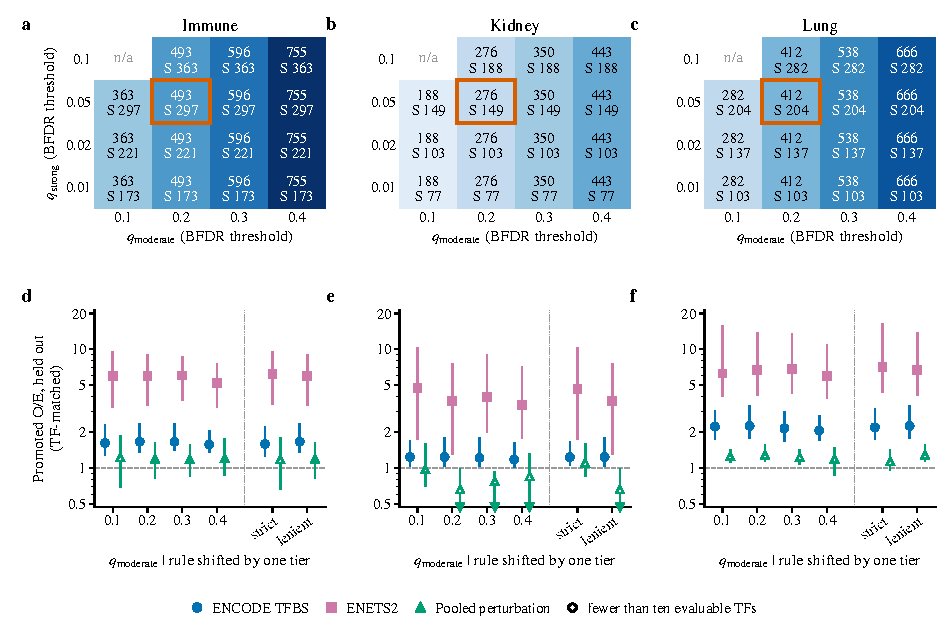
\includegraphics[width=\textwidth]{figS4_gov_grid.pdf}
  \caption{\textbf{Sensitivity of claim governance to the BFDR thresholds} (dual-universe rule). (a--c) Number of promoted edges (Strong $\cup$ Moderate; colour and upper number) and of Strong edges (S) over the grid of $q_\mathrm{strong} \times q_\mathrm{moderate}$; the prespecified point is outlined. Under the primary rule $q_\mathrm{strong}$ only moves edges between Strong and Moderate, so the promoted set and its enrichment do not depend on it (largest change of O/E across $q_\mathrm{strong}$: 0.00). (d--f) Observed over TF-matched expected held-out positives in the promoted set, by $q_\mathrm{moderate}$ at the prespecified $q_\mathrm{strong}$, and for the rules shifted by one tier (strict, lenient) at the prespecified thresholds; bars: 95\% TF-cluster bootstrap intervals (triangles: lower limit below the axis range); open markers: intervals resting on fewer than ten evaluable TFs; reference line at 1.}
  \label{fig:S-gov-grid}
\end{figure}

% provenance: paper/r2/tables/tabS_deconc.tex generated by src/r2/paper_assets on 2026-10-15 04:06 from data/r2/tables/
%   gov_deconcentration_eval.csv (modified 2026-10-14 20:11): all rows
\begin{table}[htbp]
\centering
\small
\setlength{\tabcolsep}{3pt}
\caption{Deconcentration of the promoted set: the label-free chosen subset, an undeconcentrated subset of the same size (highest credibility), and the full promoted pool; TF concentration and TF-matched held-out O/E (95\% TF-cluster bootstrap interval).}
\label{tab:S-deconc}
\begin{tabular}{@{}lrrrrrrccc@{}}
\toprule
Set & Size & $\alpha$ & Mean $\bar c$ & TFs & Top TF & Evenness & ENCODE TFBS & ENETS2 & Pert. \\
\midrule
\multicolumn{10}{@{}l}{\emph{Immune}} \\
chosen & 49 & 8 & 0.983 & 48 & 0.04 & 1.00 & \begin{tabular}[t]{@{}c@{}}2.88\\[-1pt]{\scriptsize [2.05, 4.01]}\end{tabular} & \begin{tabular}[t]{@{}c@{}}8.33\\[-1pt]{\scriptsize [0.00, 26.58]}\end{tabular} & \begin{tabular}[t]{@{}c@{}}2.49\\[-1pt]{\scriptsize [0.00, 3.33]}\end{tabular} \\
same size, by credibility & 49 & 0 & 1.000 & 12 & 0.47 & 0.76 & \begin{tabular}[t]{@{}c@{}}2.16\\[-1pt]{\scriptsize [1.69, 2.73]}\end{tabular} & \begin{tabular}[t]{@{}c@{}}3.16\\[-1pt]{\scriptsize [0.00, 16.27]}\end{tabular} & \begin{tabular}[t]{@{}c@{}}1.85\\[-1pt]{\scriptsize [1.40, 2.21]}\end{tabular} \\
promoted pool & 493 & 0 & 0.796 & 74 & 0.15 & 0.82 & \begin{tabular}[t]{@{}c@{}}1.67\\[-1pt]{\scriptsize [1.35, 2.38]}\end{tabular} & \begin{tabular}[t]{@{}c@{}}5.95\\[-1pt]{\scriptsize [3.39, 9.05]}\end{tabular} & \begin{tabular}[t]{@{}c@{}}1.20\\[-1pt]{\scriptsize [0.82, 1.64]}\end{tabular} \\
chosen (Pielou criterion)$^{\dagger}$ & 49 & 4 & 0.993 & 41 & 0.04 & 0.99 & \begin{tabular}[t]{@{}c@{}}2.50\\[-1pt]{\scriptsize [1.86, 3.47]}\end{tabular} & \begin{tabular}[t]{@{}c@{}}2.85\\[-1pt]{\scriptsize [0.00, 13.10]}\end{tabular} & \begin{tabular}[t]{@{}c@{}}2.20\\[-1pt]{\scriptsize [1.09, 3.32]}\end{tabular} \\
same size (Pielou)$^{\dagger}$ & 49 & 0 & 1.000 & 12 & 0.47 & 0.76 & \begin{tabular}[t]{@{}c@{}}2.16\\[-1pt]{\scriptsize [1.69, 2.73]}\end{tabular} & \begin{tabular}[t]{@{}c@{}}3.16\\[-1pt]{\scriptsize [0.00, 16.27]}\end{tabular} & \begin{tabular}[t]{@{}c@{}}1.85\\[-1pt]{\scriptsize [1.40, 2.21]}\end{tabular} \\
\addlinespace[3pt]
\multicolumn{10}{@{}l}{\emph{Kidney}} \\
chosen & 55 & 2 & 0.979 & 38 & 0.05 & 0.97 & \begin{tabular}[t]{@{}c@{}}2.02\\[-1pt]{\scriptsize [1.41, 2.77]}\end{tabular} & \begin{tabular}[t]{@{}c@{}}14.22\\[-1pt]{\scriptsize [0.00, 31.34]}\end{tabular} & -- \\
same size, by credibility & 55 & 0 & 0.996 & 22 & 0.24 & 0.87 & \begin{tabular}[t]{@{}c@{}}1.64\\[-1pt]{\scriptsize [1.30, 2.47]}\end{tabular} & \begin{tabular}[t]{@{}c@{}}6.67\\[-1pt]{\scriptsize [2.52, 15.14]}\end{tabular} & \begin{tabular}[t]{@{}c@{}}1.67\\[-1pt]{\scriptsize [0.00, 2.11]}\end{tabular} \\
promoted pool & 276 & 0 & 0.786 & 58 & 0.14 & 0.85 & \begin{tabular}[t]{@{}c@{}}1.24\\[-1pt]{\scriptsize [1.03, 1.81]}\end{tabular} & \begin{tabular}[t]{@{}c@{}}3.66\\[-1pt]{\scriptsize [1.30, 7.65]}\end{tabular} & \begin{tabular}[t]{@{}c@{}}0.66\\[-1pt]{\scriptsize [0.00, 1.00]}\end{tabular} \\
chosen (Pielou criterion)$^{\dagger}$ & 28 & 8 & 0.992 & 28 & 0.04 & 1.00 & \begin{tabular}[t]{@{}c@{}}2.14\\[-1pt]{\scriptsize [1.15, 3.56]}\end{tabular} & \begin{tabular}[t]{@{}c@{}}14.04\\[-1pt]{\scriptsize [0.00, 49.24]}\end{tabular} & -- \\
same size (Pielou)$^{\dagger}$ & 28 & 0 & 0.999 & 13 & 0.21 & 0.90 & \begin{tabular}[t]{@{}c@{}}1.93\\[-1pt]{\scriptsize [1.37, 2.64]}\end{tabular} & \begin{tabular}[t]{@{}c@{}}4.87\\[-1pt]{\scriptsize [0.00, 16.25]}\end{tabular} & -- \\
\addlinespace[3pt]
\multicolumn{10}{@{}l}{\emph{Lung}} \\
chosen & 82 & 2 & 0.971 & 56 & 0.05 & 0.98 & \begin{tabular}[t]{@{}c@{}}2.72\\[-1pt]{\scriptsize [2.12, 3.59]}\end{tabular} & \begin{tabular}[t]{@{}c@{}}14.24\\[-1pt]{\scriptsize [3.05, 43.28]}\end{tabular} & \begin{tabular}[t]{@{}c@{}}1.23\\[-1pt]{\scriptsize [1.08, 1.44]}\end{tabular} \\
same size, by credibility & 82 & 0 & 0.994 & 29 & 0.13 & 0.91 & \begin{tabular}[t]{@{}c@{}}2.44\\[-1pt]{\scriptsize [2.03, 3.49]}\end{tabular} & \begin{tabular}[t]{@{}c@{}}6.72\\[-1pt]{\scriptsize [2.35, 24.71]}\end{tabular} & \begin{tabular}[t]{@{}c@{}}0.85\\[-1pt]{\scriptsize [0.00, 1.44]}\end{tabular} \\
promoted pool & 412 & 0 & 0.793 & 81 & 0.08 & 0.88 & \begin{tabular}[t]{@{}c@{}}2.27\\[-1pt]{\scriptsize [1.78, 3.37]}\end{tabular} & \begin{tabular}[t]{@{}c@{}}6.74\\[-1pt]{\scriptsize [4.12, 13.83]}\end{tabular} & \begin{tabular}[t]{@{}c@{}}1.29\\[-1pt]{\scriptsize [1.13, 1.57]}\end{tabular} \\
chosen (Pielou criterion)$^{\dagger}$ & 41 & 8 & 0.987 & 41 & 0.02 & 1.00 & \begin{tabular}[t]{@{}c@{}}1.68\\[-1pt]{\scriptsize [0.46, 2.87]}\end{tabular} & \begin{tabular}[t]{@{}c@{}}0.00\\[-1pt]{\scriptsize [0.00, 0.00]}\end{tabular} & 0.00 \\
same size (Pielou)$^{\dagger}$ & 41 & 0 & 0.999 & 19 & 0.15 & 0.92 & \begin{tabular}[t]{@{}c@{}}2.61\\[-1pt]{\scriptsize [2.14, 3.91]}\end{tabular} & \begin{tabular}[t]{@{}c@{}}6.61\\[-1pt]{\scriptsize [0.00, 26.88]}\end{tabular} & \begin{tabular}[t]{@{}c@{}}1.46\\[-1pt]{\scriptsize [0.00, 1.62]}\end{tabular} \\
\bottomrule
\end{tabular}
\par\smallskip
\begin{minipage}{\linewidth}\footnotesize
$\alpha$: TF penalty of the greedy selection (0: no deconcentration). Top TF: share of the set's edges belonging to its most frequent TF; evenness: Pielou's evenness of the TF counts.

$^{\dagger}$\,Post hoc: defined after the held-out data had been examined.
\end{minipage}
\end{table}

% generated by src/r2/paper_assets (make_paper_assets.py figures); do not edit by hand
% provenance: figS3_deconcentration generated by src/r2/paper_assets on 2026-10-15 04:07 from data/r2/tables/
%   gov_deconcentration.csv (modified 2026-10-14 20:11): all rows (budget fraction x alpha grid per tissue); chosen = primary label-free rule; chosen_pielou = post hoc
\begin{figure}[htbp]
  \centering
  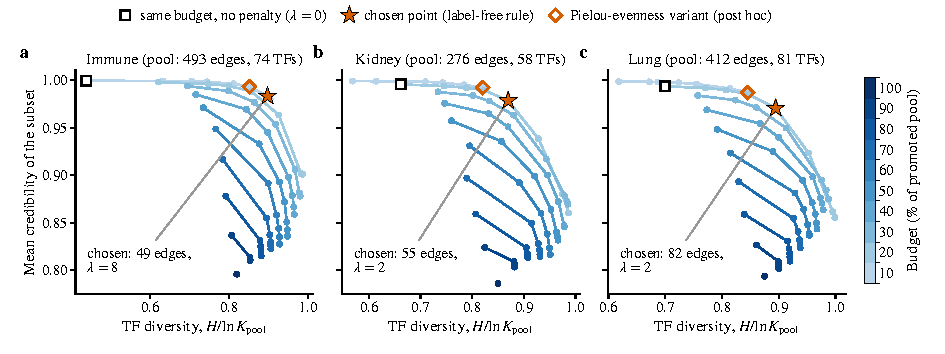
\includegraphics[width=\textwidth]{figS3_deconcentration.pdf}
  \caption{\textbf{Label-free deconcentration of the promoted set.} Each line is one budget (share of the promoted pool, colour) traced over the TF penalty $\lambda \in \{0, 0.25, 0.5, 1, 2, 4, 8, 16\}$; x: TF diversity (Shannon entropy over TFs divided by the log number of TFs in the pool), y: mean credibility of the selected subset (min of global-fit and context-fit credibility). Star: operating point chosen by the label-free rule of Section~\ref{sec:governance} (harmonic mean of normalised credibility and diversity; fixed after held-out results of other analyses existed, but no held-out data enter the choice); open square: the same budget without penalty; open diamond: the post hoc variant with Pielou evenness.}
  \label{fig:S-deconc}
\end{figure}


\clearpage
\section{Hub-bias simulation}\label{sec:S-sim}
Results of the post hoc hub-bias simulation with known truth described in Section~\ref{sec:inference} (Section~\ref{sec:res-hubs}): set sizes, error rates, precision and over-promotion for every estimator and scenario, and the posterior-mode structure of the latent-class fits.
% provenance: paper/r2/tables/tabS_simhub.tex generated by src/r2/paper_assets on 2026-10-15 04:06 from data/r2/tables/
%   sim_hub_summary.csv (modified 2026-10-14 20:37): set_rule in {bfdr05, size_matched, score}
\begin{table}[htbp]
\centering
\small
\setlength{\tabcolsep}{4pt}
\caption{Hub-bias simulation with known truth: BFDR\,$\le$\,0.05 set size and realised FDR, precision and over-promotion index of top-popularity-decile TFs at a set size matched to the Family-HB set, and AUROC over all edges (mean over replicates, 95\% $t$ interval).$^{\dagger}$}
\label{tab:S-simhub}
\begin{tabular}{@{}lrrccc@{}}
\toprule
 & \multicolumn{2}{c}{BFDR\,$\le$\,0.05 set} & \multicolumn{2}{c}{Size-matched set} &  \\
\cmidrule(lr){2-3}\cmidrule(lr){4-5}
Method & Size & FDR & Precision [95\% CI] & Index [95\% CI] & AUROC \\
\midrule
\multicolumn{6}{@{}l}{\emph{Truth independent of popularity}} \\
Oracle posterior & 2{,}902 & 0.07 & 0.98 [0.97, 0.99] & 4.65 [4.31, 5.00] & 0.909 \\
Family-HB & 1{,}094 & 0.07 & 0.93 [0.92, 0.95] & 5.09 [4.57, 5.61] & 0.858 \\
EM baseline & 5{,}518 & 0.23 & 0.89 [0.87, 0.90] & 6.62 [5.94, 7.31] & 0.858 \\
Dependence-aware & 201 & 0.10 & 0.79 [0.74, 0.84] & 3.38 [2.70, 4.07] & 0.856 \\
Family-regularized & 5{,}517 & 0.23 & 0.89 [0.87, 0.90] & 6.62 [5.94, 7.31] & 0.858 \\
Union & -- & -- & 0.38 [0.37, 0.39] & 1.98 [1.88, 2.08] & 0.803 \\
Majority ($\geq$2) & -- & -- & 0.72 [0.71, 0.73] & 2.58 [2.49, 2.68] & 0.682 \\
Vote fraction & -- & -- & 0.61 [0.58, 0.64] & 1.44 [1.12, 1.77] & 0.805 \\
Fisher & -- & -- & 0.90 [0.88, 0.91] & 6.29 [5.62, 6.95] & 0.839 \\
Stouffer & -- & -- & 0.89 [0.87, 0.91] & 5.99 [5.35, 6.62] & 0.836 \\
Family-HB + observation ($n$ = 5) & 115{,}475 & 1.00 & 0.00 [0.00, 0.00] & 7.95 [5.43, 10.46] & 0.255 \\
EM + observation & 55{,}172 & 0.70 & 0.86 [0.84, 0.89] & 6.43 [5.77, 7.10] & 0.817 \\
\addlinespace[3pt]
\multicolumn{6}{@{}l}{\emph{Biological hubs}} \\
Oracle posterior & 4{,}671 & 0.07 & 0.98 [0.97, 0.99] & 3.36 [3.10, 3.63] & 0.923 \\
Family-HB & 1{,}842 & 0.08 & 0.92 [0.89, 0.94] & 2.99 [2.62, 3.36] & 0.886 \\
EM baseline & 7{,}635 & 0.24 & 0.92 [0.91, 0.94] & 3.95 [3.57, 4.33] & 0.887 \\
Dependence-aware & 168 & 0.02 & 0.90 [0.86, 0.93] & 3.02 [2.59, 3.45] & 0.884 \\
Family-regularized & 7{,}634 & 0.24 & 0.92 [0.91, 0.94] & 3.95 [3.57, 4.33] & 0.887 \\
Union & -- & -- & 0.42 [0.41, 0.43] & 1.34 [1.28, 1.39] & 0.849 \\
Majority ($\geq$2) & -- & -- & 0.77 [0.76, 0.78] & 1.89 [1.82, 1.96] & 0.737 \\
Vote fraction & -- & -- & 0.70 [0.65, 0.74] & 1.59 [1.38, 1.80] & 0.851 \\
Fisher & -- & -- & 0.92 [0.91, 0.94] & 3.80 [3.42, 4.18] & 0.876 \\
Stouffer & -- & -- & 0.92 [0.90, 0.94] & 3.69 [3.33, 4.04] & 0.873 \\
Family-HB + observation ($n$ = 4) & 146{,}534 & 1.00 & 0.00 [0.00, 0.00] & 3.04 [2.02, 4.06] & 0.208 \\
EM + observation & 85{,}709 & 0.87 & 0.90 [0.88, 0.92] & 3.88 [3.52, 4.24] & 0.835 \\
\addlinespace[3pt]
\multicolumn{6}{@{}l}{\emph{Hub-concentrated literature copying}} \\
Oracle posterior & 1{,}195 & 0.06 & 0.96 [0.95, 0.97] & 2.69 [2.55, 2.84] & 0.907 \\
Family-HB & 784 & 0.23 & 0.77 [0.70, 0.84] & 5.34 [4.70, 5.97] & 0.864 \\
EM baseline & 10{,}778 & 0.54 & 0.41 [0.36, 0.45] & 9.01 [8.63, 9.38] & 0.863 \\
Dependence-aware & 172 & 0.47 & 0.60 [0.55, 0.66] & 5.44 [4.34, 6.53] & 0.862 \\
Family-regularized & 10{,}775 & 0.54 & 0.41 [0.36, 0.45] & 9.01 [8.63, 9.38] & 0.863 \\
Union & -- & -- & 0.31 [0.30, 0.32] & 2.61 [2.47, 2.76] & 0.799 \\
Majority ($\geq$2) & -- & -- & 0.46 [0.45, 0.47] & 3.94 [3.76, 4.12] & 0.679 \\
Vote fraction & -- & -- & 0.47 [0.46, 0.48] & 1.33 [0.96, 1.71] & 0.800 \\
Fisher & -- & -- & 0.46 [0.42, 0.50] & 8.59 [8.20, 8.98] & 0.848 \\
Stouffer & -- & -- & 0.48 [0.43, 0.52] & 8.20 [7.78, 8.62] & 0.846 \\
Family-HB + observation ($n$ = 3) & 79{,}154 & 1.00 & 0.00 [0.00, 0.00] & 6.17 [3.28, 9.07] & 0.267 \\
EM + observation & 11{,}770 & 0.55 & 0.42 [0.37, 0.46] & 9.00 [8.63, 9.38] & 0.873 \\
\bottomrule
\end{tabular}
\par\smallskip
\begin{minipage}{\linewidth}\footnotesize
Over-promotion index: share of the set at top-popularity-decile TFs divided by the share of true edges there (1 = proportional to biology). $n$: replicates behind a row when fewer than the design. Precision intervals are truncated at 0.

$^{\dagger}$\,Post hoc: defined after the held-out data had been examined.
\end{minipage}
\end{table}

% provenance: paper/r2/tables/tabS_simhub_modes.tex generated by src/r2/paper_assets on 2026-10-15 04:06 from data/r2/tables/
%   sim_hub_modes.csv (modified 2026-10-14 20:37): all rows
\begin{table}[htbp]
\centering
\small
\setlength{\tabcolsep}{3.5pt}
\caption{Posterior-mode structure of the latent-class fits in the hub-bias simulation: restarts reaching the best optimum, distinct optima, median gap to the next optimum, selected optima that are label-swapped or have an inflated true class, and the fitted class weight.$^{\dagger}$}
\label{tab:S-simhub-modes}
\begin{tabular}{@{}lrrrrrrrrr@{}}
\toprule
Model & Reps & Restarts & At best & Optima & Gap & Swapped & Inflated & $w_{\mathrm T}$ & Truth \\
\midrule
\multicolumn{10}{@{}l}{\emph{Truth independent of popularity}} \\
EM baseline & 20 & 10 & 1.00 & 1.0 & -- & 0 & 0 & 0.01 & 0.0099 \\
Dependence-aware & 20 & 10 & 0.87 & 1.4 & 3.3 & 13 & 0 & 0.0017 & 0.0099 \\
Family-regularized & 20 & 10 & 0.98 & 1.1 & 14814.4 & 0 & 0 & 0.01 & 0.0099 \\
Family-HB & 20 & 30 & 0.43 & 4.1 & 10.8 & 0 & 0 & 0.0085 & 0.0099 \\
EM + observation & 20 & 10 & 0.43 & 1.8 & 8129.8 & 0 & 14 & 0.38 & 0.0099 \\
Family-HB + observation & 5 & 20 & 0.49 & 4.8 & 4310.6 & 5 & 5 & 0.50 & 0.01 \\
\addlinespace[3pt]
\multicolumn{10}{@{}l}{\emph{Biological hubs}} \\
EM baseline & 20 & 10 & 1.00 & 1.0 & -- & 0 & 0 & 0.01 & 0.01 \\
Dependence-aware & 20 & 10 & 0.99 & 1.1 & 6.4 & 5 & 0 & 0.0043 & 0.01 \\
Family-regularized & 20 & 10 & 0.94 & 1.6 & 27797.1 & 0 & 0 & 0.01 & 0.01 \\
Family-HB & 20 & 30 & 0.48 & 3.4 & 12.4 & 0 & 0 & 0.0098 & 0.01 \\
EM + observation & 20 & 10 & 0.27 & 1.9 & 11950.6 & 0 & 19 & 0.36 & 0.01 \\
Family-HB + observation & 4 & 20 & 0.64 & 3.5 & 3464.2 & 4 & 4 & 0.42 & 0.0099 \\
\addlinespace[3pt]
\multicolumn{10}{@{}l}{\emph{Hub-concentrated literature copying}} \\
EM baseline & 20 & 10 & 1.00 & 1.0 & -- & 0 & 0 & 0.02 & 0.0098 \\
Dependence-aware & 20 & 10 & 0.93 & 1.2 & 14.3 & 1 & 0 & 0.0038 & 0.0098 \\
Family-regularized & 20 & 10 & 0.96 & 1.4 & 33702.0 & 0 & 0 & 0.02 & 0.0098 \\
Family-HB & 20 & 30 & 0.56 & 3.4 & 60.8 & 0 & 0 & 0.0087 & 0.0098 \\
EM + observation & 20 & 10 & 0.90 & 1.6 & 4692.2 & 0 & 1 & 0.01 & 0.0098 \\
Family-HB + observation & 3 & 20 & 0.52 & 3.0 & 6881.6 & 3 & 3 & 0.37 & 0.0097 \\
\bottomrule
\end{tabular}
\par\smallskip
\begin{minipage}{\linewidth}\footnotesize
$^{\dagger}$\,Post hoc: defined after the held-out data had been examined.
\end{minipage}
\end{table}


\clearpage
\section{Replication check}\label{sec:S-rep}
The pooled Bayesian replication model of Section~\ref{sec:replication}: per-study posterior summaries, dependence on the priors, and the leave-$k$-out refits (Section~\ref{sec:res-replication}).
% provenance: paper/r2/tables/tabS_rep_bayes.tex generated by src/r2/paper_assets on 2026-10-15 04:06 from data/r2/tables/
%   rep_bayes.csv (modified 2026-10-14 20:18): level == study
\begin{table}[htbp]
\centering
\small
\caption{Pooled replication model under the primary prior (study level): per-study odds ratio $\exp(\theta_u)$ (posterior median, 95\% CrI) and pass probability, beside the per-study frequentist estimates.}
\label{tab:S-rep-bayes}
\begin{tabular}{@{}lccrrrr@{}}
\toprule
Study & OR [95\% CrI] & $P$(pass) & O/E & MH OR & Observed & Expected \\
\midrule
Dixit 2016 & 2.74 [0.84, 5.23] & 0.89 & 0.00 & 0.00 & 0 & 0.21 \\
Norman 2019 & 3.07 [2.37, 3.96] & 1.00 & 1.95 & 3.27 & 100 & 51 \\
Papalexi 2021 & 3.46 [2.64, 4.69] & 1.00 & 2.24 & 3.64 & 84 & 38 \\
Replogle 2022 & 2.43 [1.54, 3.42] & 0.98 & 1.57 & 2.07 & 38 & 24 \\
\midrule
Pooled, $\exp(\mu)$ & 2.82 [1.42, 4.09] & 0.97 & -- & -- & -- & -- \\
New study, $\exp(\theta_{\mathrm{new}})$ & 2.89 [0.92, 6.56] & 0.92 & -- & -- & -- & -- \\
\bottomrule
\end{tabular}
\par\smallskip
\begin{minipage}{\linewidth}\footnotesize
Between-study SD $\sigma$: 0.32 [0.02, 0.88]; max.\ $\widehat R$ 1.007, min.\ bulk ESS 1{,}286, 0 divergent transitions.
\end{minipage}
\end{table}

% provenance: paper/r2/tables/tabS_rep_prior.tex generated by src/r2/paper_assets on 2026-10-15 04:06 from data/r2/tables/
%   rep_prior_sensitivity.csv (modified 2026-10-14 20:18): level == study
\begin{table}[htbp]
\centering
\small
\setlength{\tabcolsep}{3.5pt}
\caption{Prior sensitivity of the pooled replication model (study level): pooled odds ratio $\exp(\mu)$ and odds ratio of a new study $\exp(\theta_{\mathrm{new}})$ (posterior median, 95\% CrI), between-study SD $\sigma$, posterior probability that the pooled odds ratio reaches the endpoint, and each study's posterior probability of passing.}
\label{tab:S-rep-prior}
\begin{tabular}{@{}lcccccccc@{}}
\toprule
Profile & $\exp(\mu)$ & $P$(end- & $\sigma$ & $\exp(\theta_{\mathrm{new}})$ & \multicolumn{4}{c}{Pass probability} \\
\cmidrule(lr){6-9}
($\mu$, $\sigma$ priors) & & point) & & & Dixit & Norman & Papalexi & Replogle \\
\midrule
\begin{tabular}[t]{@{}l@{}}primary\\[-1pt]{\scriptsize N(0, 1), HN(0.5)}\end{tabular} & \begin{tabular}[t]{@{}c@{}}2.82\\[-1pt]{\scriptsize [1.42, 4.09]}\end{tabular} & 0.97 & \begin{tabular}[t]{@{}c@{}}0.32\\[-1pt]{\scriptsize [0.02, 0.88]}\end{tabular} & \begin{tabular}[t]{@{}c@{}}2.89\\[-1pt]{\scriptsize [0.92, 6.56]}\end{tabular} & 0.89 & 1.00 & 1.00 & 0.98 \\
\begin{tabular}[t]{@{}l@{}}mu sd0.5\\[-1pt]{\scriptsize N(0, 0.5), HN(0.5)}\end{tabular} & \begin{tabular}[t]{@{}c@{}}2.43\\[-1pt]{\scriptsize [1.11, 3.50]}\end{tabular} & 0.90 & \begin{tabular}[t]{@{}c@{}}0.41\\[-1pt]{\scriptsize [0.03, 1.04]}\end{tabular} & \begin{tabular}[t]{@{}c@{}}2.53\\[-1pt]{\scriptsize [0.57, 6.12]}\end{tabular} & 0.79 & 1.00 & 1.00 & 0.97 \\
\begin{tabular}[t]{@{}l@{}}mu sd2\\[-1pt]{\scriptsize N(0, 2), HN(0.5)}\end{tabular} & \begin{tabular}[t]{@{}c@{}}2.90\\[-1pt]{\scriptsize [1.55, 4.36]}\end{tabular} & 0.98 & \begin{tabular}[t]{@{}c@{}}0.31\\[-1pt]{\scriptsize [0.02, 0.85]}\end{tabular} & \begin{tabular}[t]{@{}c@{}}2.92\\[-1pt]{\scriptsize [1.06, 6.85]}\end{tabular} & 0.91 & 1.00 & 1.00 & 0.98 \\
\begin{tabular}[t]{@{}l@{}}sigma hn0.25\\[-1pt]{\scriptsize N(0, 1), HN(0.25)}\end{tabular} & \begin{tabular}[t]{@{}c@{}}2.91\\[-1pt]{\scriptsize [1.97, 3.92]}\end{tabular} & 0.99 & \begin{tabular}[t]{@{}c@{}}0.21\\[-1pt]{\scriptsize [0.01, 0.51]}\end{tabular} & \begin{tabular}[t]{@{}c@{}}2.92\\[-1pt]{\scriptsize [1.43, 5.06]}\end{tabular} & 0.96 & 1.00 & 1.00 & 0.99 \\
\begin{tabular}[t]{@{}l@{}}sigma hn1\\[-1pt]{\scriptsize N(0, 1), HN(1)}\end{tabular} & \begin{tabular}[t]{@{}c@{}}2.72\\[-1pt]{\scriptsize [1.01, 4.27]}\end{tabular} & 0.92 & \begin{tabular}[t]{@{}c@{}}0.47\\[-1pt]{\scriptsize [0.04, 1.48]}\end{tabular} & \begin{tabular}[t]{@{}c@{}}2.78\\[-1pt]{\scriptsize [0.49, 8.78]}\end{tabular} & 0.81 & 1.00 & 1.00 & 0.97 \\
\begin{tabular}[t]{@{}l@{}}skeptical\\[-1pt]{\scriptsize N(0, 0.2), HN(0.5)}\end{tabular} & \begin{tabular}[t]{@{}c@{}}1.21\\[-1pt]{\scriptsize [0.81, 1.81]}\end{tabular} & 0.15 & \begin{tabular}[t]{@{}c@{}}0.77\\[-1pt]{\scriptsize [0.38, 1.28]}\end{tabular} & \begin{tabular}[t]{@{}c@{}}1.28\\[-1pt]{\scriptsize [0.21, 6.42]}\end{tabular} & 0.33 & 1.00 & 1.00 & 0.91 \\
\begin{tabular}[t]{@{}l@{}}skeptical sigma0.25\\[-1pt]{\scriptsize N(0, 0.2), HN(0.25)}\end{tabular} & \begin{tabular}[t]{@{}c@{}}1.38\\[-1pt]{\scriptsize [0.92, 2.06]}\end{tabular} & 0.34 & \begin{tabular}[t]{@{}c@{}}0.52\\[-1pt]{\scriptsize [0.26, 0.82]}\end{tabular} & \begin{tabular}[t]{@{}c@{}}1.43\\[-1pt]{\scriptsize [0.42, 4.04]}\end{tabular} & 0.41 & 1.00 & 1.00 & 0.90 \\
\begin{tabular}[t]{@{}l@{}}diffuse\\[-1pt]{\scriptsize N(0, 2), HN(1)}\end{tabular} & \begin{tabular}[t]{@{}c@{}}2.87\\[-1pt]{\scriptsize [1.28, 4.79]}\end{tabular} & 0.96 & \begin{tabular}[t]{@{}c@{}}0.44\\[-1pt]{\scriptsize [0.04, 1.35]}\end{tabular} & \begin{tabular}[t]{@{}c@{}}2.88\\[-1pt]{\scriptsize [0.55, 9.07]}\end{tabular} & 0.84 & 1.00 & 1.00 & 0.97 \\
\begin{tabular}[t]{@{}l@{}}tf random slope$^{\dagger}$\\[-1pt]{\scriptsize N(0, 1), HN(0.5)}\end{tabular} & \begin{tabular}[t]{@{}c@{}}3.28\\[-1pt]{\scriptsize [1.71, 5.42]}\end{tabular} & 0.99 & \begin{tabular}[t]{@{}c@{}}0.29\\[-1pt]{\scriptsize [0.01, 0.91]}\end{tabular} & \begin{tabular}[t]{@{}c@{}}3.31\\[-1pt]{\scriptsize [1.02, 7.99]}\end{tabular} & 0.93 & 1.00 & 1.00 & 1.00 \\
\bottomrule
\end{tabular}
\par\smallskip
\begin{minipage}{\linewidth}\footnotesize
N, HN: normal and half-normal priors of $\mu$ and $\sigma$. Pass probability: posterior probability that the study's odds ratio reaches the endpoint. tf random slope: adds a TF-level random slope. Max.\ $\widehat R$ 1.007 under the primary prior.

$^{\dagger}$\,Post hoc: defined after the held-out data had been examined.
\end{minipage}
\end{table}

% provenance: paper/r2/tables/tabS_rep_leavek.tex generated by src/r2/paper_assets on 2026-10-15 04:06 from data/r2/tables/
%   rep_leavek.csv (modified 2026-10-14 20:24): row_type == summary
\begin{table}[htbp]
\centering
\small
\caption{Leave-$k$-out refits of the pooled replication model: changes in the pooled log odds ratio $\mu$, in the posterior probability that the pooled odds ratio reaches the endpoint, and in the per-unit pass probabilities, over all subsets of $k$ units left out.}
\label{tab:S-rep-leavek}
\begin{tabular}{@{}lrrrrrrr@{}}
\toprule
 & & \multicolumn{2}{c}{$|\Delta\mu|$} & \multicolumn{2}{c}{$|\Delta P|$} & \multicolumn{2}{c}{$|\Delta$ pass prob.$|$} \\
\cmidrule(lr){3-4}\cmidrule(lr){5-6}\cmidrule(lr){7-8}
Scheme & Fits & mean & max & mean & max & mean & max \\
\midrule
\multicolumn{8}{@{}l}{\emph{Study level (full data: $\mu$ = 1.00, $P$ = 0.97)}} \\
L1O & 4 & 0.10 & 0.15 & 0.03 & 0.06 & 0.02 & 0.09 \\
L2O & 6 & 0.16 & 0.45 & 0.10 & 0.29 & 0.05 & 0.26 \\
L3O & 4 & 0.45 & 1.24 & 0.27 & 0.72 & 0.17 & 0.63 \\
\addlinespace[3pt]
\multicolumn{8}{@{}l}{\emph{Cohort level (full data: $\mu$ = 1.01, $P$ = 0.97)}} \\
L1O & 5 & 0.09 & 0.17 & 0.03 & 0.07 & 0.02 & 0.11 \\
L2O & 10 & 0.14 & 0.46 & 0.07 & 0.28 & 0.05 & 0.26 \\
L3O & 10 & 0.28 & 1.25 & 0.17 & 0.74 & 0.12 & 0.66 \\
\bottomrule
\end{tabular}
\end{table}

% generated by src/r2/paper_assets (make_paper_assets.py figures); do not edit by hand
% provenance: figS8_replication_leavek generated by src/r2/paper_assets on 2026-10-15 04:07 from data/r2/tables/
%   rep_leavek.csv (modified 2026-10-14 20:24): row_type == 'fit'; levels study and cohort; columns k, left_out, units_kept, mu_mean, mu_q025, mu_q975, degenerate_single_unit
%   rep_bayes.csv (modified 2026-10-14 20:18): profile == 'primary', parameter == 'mu' (full fit with all units)
\begin{figure}[htbp]
  \centering
  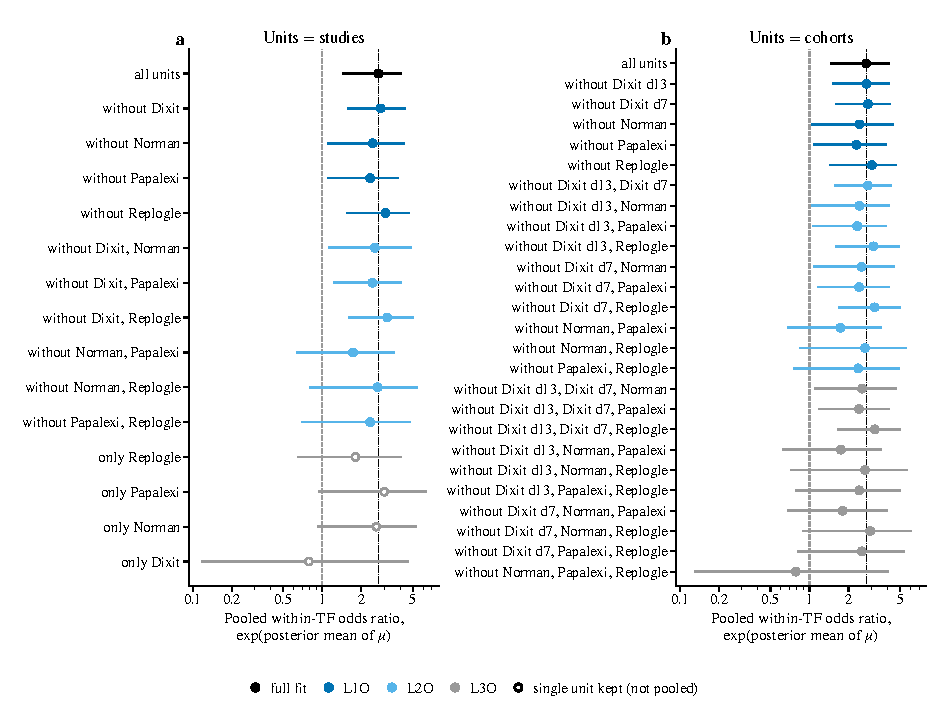
\includegraphics[width=\textwidth]{figS8_replication_leavek.pdf}
  \caption{\textbf{Leave-$k$-out drift of the pooled replication effect.} Points: $\exp$ of the posterior mean of the pooled within-TF log odds ratio $\mu$ of the Bayesian random-effects model, with the exponentiated 95\% credible limits (prior $\mu\sim N(0,1^2)$, $\sigma\sim HN(0.5)$), for the full data and refitted after removing every subset of one (L1O), two (L2O) or three (L3O) units, with studies (a) or cohorts (b) as units; the main text reports the posterior median of $\exp(\mu)$, which is 2.82 at study level against 2.71 for the mean shown here. Open markers: fits that keep a single unit, whose $\mu$ is that unit's effect shrunk towards the prior rather than a pooled estimate. Dashed line: no enrichment; dotted line: full-data posterior mean.}
  \label{fig:S-leavek}
\end{figure}


\clearpage
\section{Computation}\label{sec:S-compute}
Scaling exponents measured on synthetic evidence and the complexity of each computational stage (Section~\ref{sec:res-compute}).
% provenance: paper/r2/tables/tabS_scaling.tex generated by src/r2/paper_assets on 2026-10-15 04:06 from data/r2/tables/
%   scale_fits.csv (modified 2026-10-14 20:38): form == log-log
\begin{table}[htbp]
\centering
\small
\setlength{\tabcolsep}{3pt}
\caption{Empirical scaling exponents from the compute-scaling experiment: least-squares fits of $\log_{10} y = a + b \log_{10} x$ over the synthetic configurations (slope $b$ with standard error, $R^2$, number of configurations).}
\label{tab:S-scaling}
\begin{tabular}{@{}p{5.2cm}p{4.2cm}rcr@{}}
\toprule
Quantity $y$ vs $x$ & Configurations & $n$ & Slope (SE) & $R^2$ \\
\midrule
\multicolumn{5}{@{}l}{\emph{Measurement session a}} \\
\parbox[t]{5.2cm}{\raggedright $P$ vs $N$\strut} & \parbox[t]{4.2cm}{\raggedright\footnotesize independent streaming compression $K=10$\strut} & 3 & 0.47 (0.01) & 1.00 \\
\parbox[t]{5.2cm}{\raggedright $P$ vs $N$\strut} & \parbox[t]{4.2cm}{\raggedright\footnotesize independent streaming compression $K=21$\strut} & 4 & 0.49 (0.01) & 1.00 \\
\parbox[t]{5.2cm}{\raggedright $P$ vs $N$\strut} & \parbox[t]{4.2cm}{\raggedright\footnotesize independent streaming compression $K=42$\strut} & 3 & 0.57 (0.01) & 1.00 \\
\parbox[t]{5.2cm}{\raggedright $P$ vs $N$\strut} & \parbox[t]{4.2cm}{\raggedright\footnotesize template streaming compression $K=10$\strut} & 3 & 0.52 (0.02) & 1.00 \\
\parbox[t]{5.2cm}{\raggedright $P$ vs $N$\strut} & \parbox[t]{4.2cm}{\raggedright\footnotesize template streaming compression $K=21$\strut} & 5 & 0.63 (0.01) & 1.00 \\
\parbox[t]{5.2cm}{\raggedright $P$ vs $N$\strut} & \parbox[t]{4.2cm}{\raggedright\footnotesize template streaming compression $K=42$\strut} & 4 & 0.65 (0.01) & 1.00 \\
\parbox[t]{5.2cm}{\raggedright $P$ vs $N$\strut} & \parbox[t]{4.2cm}{\raggedright\footnotesize template whole-matrix compression $K=21$\strut} & 4 & 0.62 (0.01) & 1.00 \\
\parbox[t]{5.2cm}{\raggedright compression wall time vs $N$\strut} & \parbox[t]{4.2cm}{\raggedright\footnotesize streaming compression, all K and generators\strut} & 22 & 1.09 (0.07) & 0.93 \\
\parbox[t]{5.2cm}{\raggedright compression wall time vs $NK$\strut} & \parbox[t]{4.2cm}{\raggedright\footnotesize streaming compression, all K and generators\strut} & 22 & 1.07 (0.02) & 0.99 \\
\parbox[t]{5.2cm}{\raggedright peak RSS vs $N$\strut} & \parbox[t]{4.2cm}{\raggedright\footnotesize streaming compression, all K and generators\strut} & 22 & 0.29 (0.02) & 0.92 \\
\parbox[t]{5.2cm}{\raggedright compression wall time vs $N$\strut} & \parbox[t]{4.2cm}{\raggedright\footnotesize whole-matrix compression, all K and generators\strut} & 4 & 1.19 (0.06) & 0.99 \\
\parbox[t]{5.2cm}{\raggedright compression wall time vs $NK$\strut} & \parbox[t]{4.2cm}{\raggedright\footnotesize whole-matrix compression, all K and generators\strut} & 4 & 1.19 (0.06) & 0.99 \\
\parbox[t]{5.2cm}{\raggedright peak RSS vs $N$\strut} & \parbox[t]{4.2cm}{\raggedright\footnotesize whole-matrix compression, all K and generators\strut} & 4 & 0.45 (0.03) & 0.99 \\
\parbox[t]{5.2cm}{\raggedright log posterior and gradient time vs $PKS$\strut} & \parbox[t]{4.2cm}{\raggedright\footnotesize all\strut} & 26 & 0.56 (0.04) & 0.90 \\
\parbox[t]{5.2cm}{\raggedright L-BFGS evaluation time vs $PKS$\strut} & \parbox[t]{4.2cm}{\raggedright\footnotesize all\strut} & 25 & 0.39 (0.03) & 0.87 \\
\parbox[t]{5.2cm}{\raggedright MAP, 10 restarts, time vs $PKS$\strut} & \parbox[t]{4.2cm}{\raggedright\footnotesize all, measured or extrapolated\strut} & 25 & 0.56 (0.05) & 0.84 \\
\parbox[t]{5.2cm}{\raggedright MAP peak RSS vs $PK$\strut} & \parbox[t]{4.2cm}{\raggedright\footnotesize all\strut} & 26 & 0.25 (0.03) & 0.75 \\
\parbox[t]{5.2cm}{\raggedright log posterior and gradient time vs $PKS$\strut} & \parbox[t]{4.2cm}{\raggedright\footnotesize $P\geq 10^{4}$\strut} & 12 & 0.84 (0.06) & 0.95 \\
\parbox[t]{5.2cm}{\raggedright L-BFGS evaluation time vs $PKS$\strut} & \parbox[t]{4.2cm}{\raggedright\footnotesize $P\geq 10^{4}$\strut} & 11 & 0.63 (0.05) & 0.95 \\
\parbox[t]{5.2cm}{\raggedright MAP, 10 restarts, time vs $PKS$\strut} & \parbox[t]{4.2cm}{\raggedright\footnotesize $P\geq 10^{4}$, measured or extrapolated\strut} & 11 & 0.90 (0.12) & 0.87 \\
\parbox[t]{5.2cm}{\raggedright MAP peak RSS vs $PK$\strut} & \parbox[t]{4.2cm}{\raggedright\footnotesize $P\geq 10^{4}$\strut} & 12 & 0.50 (0.04) & 0.93 \\
\parbox[t]{5.2cm}{\raggedright MAP evaluations per restart vs $N$\strut} & \parbox[t]{4.2cm}{\raggedright\footnotesize template and independent generators, restarts run\strut} & 22 & 0.42 (0.02) & 0.95 \\
\parbox[t]{5.2cm}{\raggedright MAP evaluations per restart vs $P$\strut} & \parbox[t]{4.2cm}{\raggedright\footnotesize template and independent generators, restarts run\strut} & 22 & 0.40 (0.06) & 0.71 \\
\parbox[t]{5.2cm}{\raggedright NUTS time per leapfrog step (compile excluded) vs $PKS$\strut} & \parbox[t]{4.2cm}{\raggedright\footnotesize measured\strut} & 8 & 0.80 (0.05) & 0.98 \\
\parbox[t]{5.2cm}{\raggedright NUTS, 2 chains $\times$ (300 + 300) wall time vs $PKS$\strut} & \parbox[t]{4.2cm}{\raggedright\footnotesize measured\strut} & 8 & 0.81 (0.14) & 0.85 \\
\parbox[t]{5.2cm}{\raggedright NUTS leapfrog steps per iteration vs $N$\strut} & \parbox[t]{4.2cm}{\raggedright\footnotesize measured\strut} & 8 & 0.36 (0.03) & 0.96 \\
\bottomrule
\end{tabular}
\end{table}

\begin{table}[htbp]
\ContinuedFloat
\centering
\small
\setlength{\tabcolsep}{3pt}
\caption{Empirical scaling exponents from the compute-scaling experiment: least-squares fits of $\log_{10} y = a + b \log_{10} x$ over the synthetic configurations (slope $b$ with standard error, $R^2$, number of configurations). (continued)}
\label{tab:S-scaling-b}
\begin{tabular}{@{}p{5.2cm}p{4.2cm}rcr@{}}
\toprule
Quantity $y$ vs $x$ & Configurations & $n$ & Slope (SE) & $R^2$ \\
\midrule
\multicolumn{5}{@{}l}{\emph{Measurement session b$^{\dagger}$}} \\
\parbox[t]{5.2cm}{\raggedright compression wall time vs $N$\strut} & \parbox[t]{4.2cm}{\raggedright\footnotesize streaming compression, all K and generators\strut} & 22 & 0.90 (0.10) & 0.82 \\
\parbox[t]{5.2cm}{\raggedright compression wall time vs $NK$\strut} & \parbox[t]{4.2cm}{\raggedright\footnotesize streaming compression, all K and generators\strut} & 22 & 0.88 (0.08) & 0.87 \\
\parbox[t]{5.2cm}{\raggedright peak RSS vs $N$\strut} & \parbox[t]{4.2cm}{\raggedright\footnotesize streaming compression, all K and generators\strut} & 22 & 0.28 (0.02) & 0.93 \\
\parbox[t]{5.2cm}{\raggedright compression wall time vs $N$\strut} & \parbox[t]{4.2cm}{\raggedright\footnotesize whole-matrix compression, all K and generators\strut} & 4 & 0.86 (0.08) & 0.98 \\
\parbox[t]{5.2cm}{\raggedright compression wall time vs $NK$\strut} & \parbox[t]{4.2cm}{\raggedright\footnotesize whole-matrix compression, all K and generators\strut} & 4 & 0.86 (0.08) & 0.98 \\
\parbox[t]{5.2cm}{\raggedright peak RSS vs $N$\strut} & \parbox[t]{4.2cm}{\raggedright\footnotesize whole-matrix compression, all K and generators\strut} & 4 & 0.44 (0.06) & 0.97 \\
\parbox[t]{5.2cm}{\raggedright log posterior and gradient time vs $PKS$\strut} & \parbox[t]{4.2cm}{\raggedright\footnotesize all\strut} & 26 & 0.51 (0.05) & 0.81 \\
\parbox[t]{5.2cm}{\raggedright log posterior and gradient time (minimum) vs $PKS$\strut} & \parbox[t]{4.2cm}{\raggedright\footnotesize all\strut} & 26 & 0.61 (0.04) & 0.90 \\
\parbox[t]{5.2cm}{\raggedright L-BFGS evaluation time vs $PKS$\strut} & \parbox[t]{4.2cm}{\raggedright\footnotesize all\strut} & 19 & 0.23 (0.04) & 0.71 \\
\parbox[t]{5.2cm}{\raggedright MAP, 10 restarts, time vs $PKS$\strut} & \parbox[t]{4.2cm}{\raggedright\footnotesize all, measured or extrapolated\strut} & 19 & 0.29 (0.07) & 0.54 \\
\parbox[t]{5.2cm}{\raggedright MAP peak RSS vs $PK$\strut} & \parbox[t]{4.2cm}{\raggedright\footnotesize all\strut} & 26 & 0.23 (0.02) & 0.79 \\
\parbox[t]{5.2cm}{\raggedright log posterior and gradient time vs $PKS$\strut} & \parbox[t]{4.2cm}{\raggedright\footnotesize $P\geq 10^{4}$\strut} & 12 & 0.92 (0.06) & 0.96 \\
\parbox[t]{5.2cm}{\raggedright log posterior and gradient time (minimum) vs $PKS$\strut} & \parbox[t]{4.2cm}{\raggedright\footnotesize $P\geq 10^{4}$\strut} & 12 & 0.93 (0.06) & 0.96 \\
\parbox[t]{5.2cm}{\raggedright L-BFGS evaluation time vs $PKS$\strut} & \parbox[t]{4.2cm}{\raggedright\footnotesize $P\geq 10^{4}$\strut} & 5 & 0.39 (0.06) & 0.93 \\
\parbox[t]{5.2cm}{\raggedright MAP, 10 restarts, time vs $PKS$\strut} & \parbox[t]{4.2cm}{\raggedright\footnotesize $P\geq 10^{4}$, measured or extrapolated\strut} & 5 & 0.03 (0.24) & 0.00 \\
\parbox[t]{5.2cm}{\raggedright MAP peak RSS vs $PK$\strut} & \parbox[t]{4.2cm}{\raggedright\footnotesize $P\geq 10^{4}$\strut} & 12 & 0.43 (0.04) & 0.91 \\
\parbox[t]{5.2cm}{\raggedright MAP evaluations per restart vs $N$\strut} & \parbox[t]{4.2cm}{\raggedright\footnotesize template and independent generators, restarts run\strut} & 18 & 0.38 (0.02) & 0.94 \\
\parbox[t]{5.2cm}{\raggedright MAP evaluations per restart vs $P$\strut} & \parbox[t]{4.2cm}{\raggedright\footnotesize template and independent generators, restarts run\strut} & 18 & 0.35 (0.09) & 0.46 \\
\parbox[t]{5.2cm}{\raggedright NUTS time per leapfrog step (compile excluded) vs $PKS$\strut} & \parbox[t]{4.2cm}{\raggedright\footnotesize measured\strut} & 6 & 0.58 (0.04) & 0.98 \\
\parbox[t]{5.2cm}{\raggedright NUTS, 2 chains $\times$ (300 + 300) wall time vs $PKS$\strut} & \parbox[t]{4.2cm}{\raggedright\footnotesize measured\strut} & 6 & 0.62 (0.22) & 0.67 \\
\parbox[t]{5.2cm}{\raggedright NUTS leapfrog steps per iteration vs $N$\strut} & \parbox[t]{4.2cm}{\raggedright\footnotesize measured\strut} & 6 & 0.37 (0.04) & 0.95 \\
\bottomrule
\end{tabular}
\par\smallskip
\begin{minipage}{\linewidth}\footnotesize
Session b replicated session a on the same machine with one measurement process at a time. Streaming compression: patterns found TF chunk by TF chunk and merged; whole-matrix compression: one pass over the full evidence matrix.

$^{\dagger}$\,Post hoc: defined after the held-out data had been examined.
\end{minipage}
\end{table}

% provenance: paper/r2/tables/tabS_complexity.tex generated by src/r2/paper_assets on 2026-10-15 04:06 from data/r2/tables/
%   scale_complexity.csv (modified 2026-10-14 20:38): all rows
\begin{table}[htbp]
\centering
\small
\setlength{\tabcolsep}{3pt}
\caption{Time and memory complexity of each stage ($N$ edges, $K$ annotators, $P$ observation patterns, $S$ latent classes; further symbols in the notes column).}
\label{tab:S-complexity}
\begin{tabular}{@{}p{2.8cm}p{3.2cm}p{3.3cm}p{4.6cm}@{}}
\toprule
Stage & Time & Memory & Notes \\
\midrule
\parbox[t]{2.8cm}{\raggedright Evidence encoding\strut} & \parbox[t]{3.2cm}{\raggedright\footnotesize $O(NK)$\strut} & \parbox[t]{3.3cm}{\raggedright\footnotesize $O(n_c K)$ per chunk\strut} & \parbox[t]{4.6cm}{\raggedright\scriptsize the $K$ values of an edge (unobserved, unreported, reported) are packed into base-3 words\strut} \\
\parbox[t]{2.8cm}{\raggedright Pattern compression, streaming by TF chunk\strut} & \parbox[t]{3.2cm}{\raggedright\footnotesize $O(NK + N\log n_c + C P_c\log(C P_c))$\strut} & \parbox[t]{3.3cm}{\raggedright\footnotesize $O(N)$ edge-to-pattern index $+\ O(n_c K)$ chunk $+\ O(PK)$ table\strut} & \parbox[t]{4.6cm}{\raggedright\scriptsize sort-based unique per chunk of $n_c$ edges, merge of the $C$ chunk dictionaries, $O(N)$ re-indexing; hashing would give $O(NK)$ expected time\strut} \\
\parbox[t]{2.8cm}{\raggedright Pattern compression, whole matrix\strut} & \parbox[t]{3.2cm}{\raggedright\footnotesize $O(NK\log N)$\strut} & \parbox[t]{3.3cm}{\raggedright\footnotesize $O(NK)$ matrix $+\ O(N)$ sort arrays\strut} & \parbox[t]{4.6cm}{\raggedright\scriptsize row-wise unique of the full evidence matrix\strut} \\
\parbox[t]{2.8cm}{\raggedright Number of patterns $P$\strut} & \parbox[t]{3.2cm}{\raggedright\footnotesize $P\leq\min(N,\,3^K,\,M+N_{\mathrm{rep}})$\strut} & \parbox[t]{3.3cm}{\raggedright\footnotesize --\strut} & \parbox[t]{4.6cm}{\raggedright\scriptsize $M$ distinct observation masks, $N_{\mathrm{rep}}$ edges with at least one report: every unreported edge has the all-zero pattern of its mask; TF-blocked observation keeps $M$ small\strut} \\
\parbox[t]{2.8cm}{\raggedright Log posterior and gradient, one evaluation\strut} & \parbox[t]{3.2cm}{\raggedright\footnotesize $O(PKS)$\strut} & \parbox[t]{3.3cm}{\raggedright\footnotesize $O(PK)+O(PS)$\strut} & \parbox[t]{4.6cm}{\raggedright\scriptsize independent of $N$ given $P$: $N$ enters only through the pattern counts\strut} \\
\parbox[t]{2.8cm}{\raggedright MAP, multi-start L-BFGS\strut} & \parbox[t]{3.2cm}{\raggedright\footnotesize $O(RIPKS)$\strut} & \parbox[t]{3.3cm}{\raggedright\footnotesize $O(PK)+O(RP)$\strut} & \parbox[t]{4.6cm}{\raggedright\scriptsize $R$ restarts, $I$ evaluations per restart; $I$ grew with $N$ in the experiments (Table~\ref{tab:S-scaling})\strut} \\
\parbox[t]{2.8cm}{\raggedright NUTS\strut} & \parbox[t]{3.2cm}{\raggedright\footnotesize $O(CDLPKS)$\strut} & \parbox[t]{3.3cm}{\raggedright\footnotesize $O(PK + CDd)$, $+\ O(CDP)$ if credibility is stored per draw\strut} & \parbox[t]{4.6cm}{\raggedright\scriptsize $C$ chains, $D$ iterations, $L$ leapfrog steps per iteration (at most $2^{10}-1$), $d$ parameters; $L$ grew with $N$ up to the tree-depth cap\strut} \\
\parbox[t]{2.8cm}{\raggedright Posterior credibility summaries\strut} & \parbox[t]{3.2cm}{\raggedright\footnotesize $O(D'PKS)$\strut} & \parbox[t]{3.3cm}{\raggedright\footnotesize $O(D'P)$ (quantiles); $O(P)$ (streaming mean and SD)\strut} & \parbox[t]{4.6cm}{\raggedright\scriptsize $D'$ retained draws\strut} \\
\parbox[t]{2.8cm}{\raggedright Edge-level outputs\strut} & \parbox[t]{3.2cm}{\raggedright\footnotesize $O(N)$\strut} & \parbox[t]{3.3cm}{\raggedright\footnotesize $O(N)$\strut} & \parbox[t]{4.6cm}{\raggedright\scriptsize the credibility of an edge is that of its pattern (index lookup)\strut} \\
\bottomrule
\end{tabular}
\end{table}

% generated by src/r2/paper_assets (make_paper_assets.py figures); do not edit by hand
% provenance: figS5_compute_scaling generated by src/r2/paper_assets on 2026-10-15 04:07 from data/r2/tables/
%   scale_summary.csv (modified 2026-10-14 20:38): all 26 configurations; status columns map_10_status / nuts_status (measured = filled, extrapolated/projected = open)
%   scale_map.csv (modified 2026-10-14 20:38): n_restarts_run of the measured MAP records (restart count shown in panel e)
%   scale_nuts.csv (modified 2026-10-14 20:38): chains / warmup / samples of the measured NUTS records (panel f); projected configurations: min t_nuts_projected_s and max t_nuts_projected_cap_s over the measurement sessions (the range of Table tab:compute-scaling)
%   scale_environment.csv (modified 2026-10-14 20:38): key in (cpu, hw.ncpu, hw.memsize (bytes))
\begin{figure}[htbp]
  \centering
  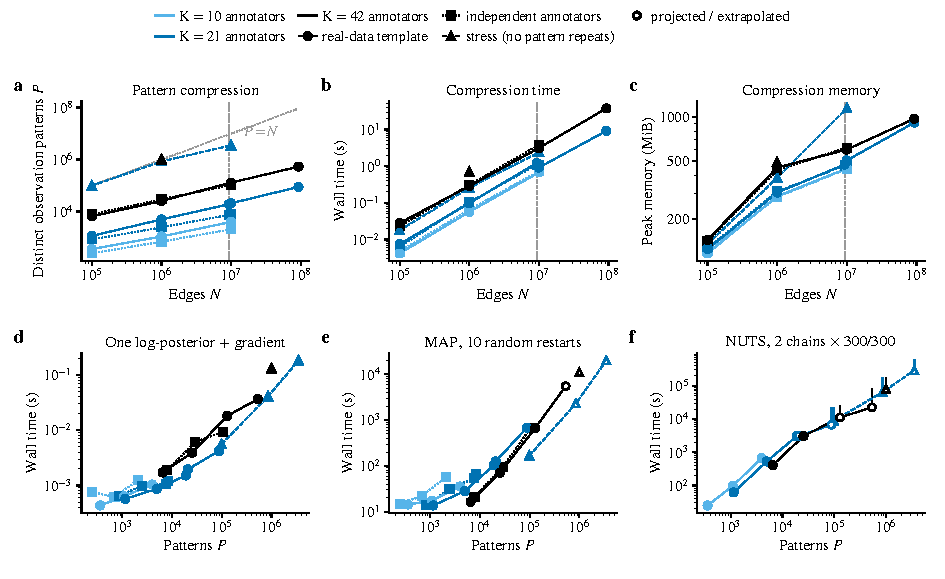
\includegraphics[width=\textwidth]{figS5_compute_scaling.pdf}
  \caption{\textbf{Computational scaling on synthetic evidence} (no held-out data). (a) Number of distinct observation patterns $P$ against the number of edges $N$ for evidence generated from the real observation design (template), from independent annotators and without repeated patterns (stress); dashed vertical line: size of the global universe. (b, c) Wall time and peak memory of the streaming pattern compression. (d) One evaluation of the collapsed log posterior and its gradient. (e) MAP with 10 random restarts (open: extrapolated from the restarts that finished, or projected from evaluation counts, a lower bound). (f) NUTS with 2 chains of 300 warm-up and 300 draws from random starts, a cost benchmark rather than a converged fit; open markers are projections from the steps per iteration of the largest measured run (lowest over the two measurement sessions), which are lower bounds because the steps per iteration grow with $N$, and the vertical bars reach the projection at the tree-depth cap (highest over the sessions), the better estimate at ten times the real size; the same ranges as in Table~\ref{tab:compute-scaling}. Measured times are wall-clock on a shared laptop (Apple M2 Pro, 10 cores, 32 GiB) and are upper bounds of the undisturbed cost.}
  \label{fig:S-scaling}
\end{figure}


\clearpage
% generated by src/r2/paper_assets/tables_supp.py (write_supp_references): entries of references.tex
% cited in the supplement; do not edit by hand
\begin{thebibliography}{99}

\bibitem[Bovolenta et~al.(2012)]{bovolenta2012htridb}
Bovolenta, L.~A., Acencio, M.~L., and Lemke, N. (2012).
\newblock HTRIdb: an open-access database for experimentally verified human transcriptional regulation interactions.
\newblock \emph{BMC Genomics}, 13(1):405.
\newblock doi:\href{https://doi.org/10.1186/1471-2164-13-405}{\nolinkurl{10.1186/1471-2164-13-405}}.

\bibitem[Carrasco Pro et~al.(2018)]{carrascopro2018cytreg}
Carrasco Pro, S., Dafonte Imedio, A., Santoso, C.~S., et~al. (2018).
\newblock Global landscape of mouse and human cytokine transcriptional regulation.
\newblock \emph{Nucleic Acids Research}, 46(18):9321--9337.
\newblock doi:\href{https://doi.org/10.1093/nar/gky787}{\nolinkurl{10.1093/nar/gky787}}.

\bibitem[Ch{\`e}neby et~al.(2018)]{cheneby2018remap}
Ch{\`e}neby, J., Gheorghe, M., Artufel, M., Mathelier, A., and Ballester, B. (2018).
\newblock ReMap 2018: an updated atlas of regulatory regions from an integrative analysis of DNA-binding ChIP-seq experiments.
\newblock \emph{Nucleic Acids Research}, 46(D1):D267--D275.
\newblock doi:\href{https://doi.org/10.1093/nar/gkx1092}{\nolinkurl{10.1093/nar/gkx1092}}.

\bibitem[Chu et~al.(2021)]{chu2021curation}
Chu, E.~C.-P., Morin, A., Chang, T.~H.~C., et~al. (2021).
\newblock Experiment level curation of transcriptional regulatory interactions in neurodevelopment.
\newblock \emph{PLOS Computational Biology}, 17(10):e1009484.
\newblock doi:\href{https://doi.org/10.1371/journal.pcbi.1009484}{\nolinkurl{10.1371/journal.pcbi.1009484}}.

\bibitem[Essaghir et~al.(2010)]{essaghir2010tfacts}
Essaghir, A., Toffalini, F., Knoops, L., et~al. (2010).
\newblock Transcription factor regulation can be accurately predicted from the presence of target gene signatures in microarray gene expression data.
\newblock \emph{Nucleic Acids Research}, 38(11):e120.
\newblock doi:\href{https://doi.org/10.1093/nar/gkq149}{\nolinkurl{10.1093/nar/gkq149}}.

\bibitem[{FANTOM Consortium and Riken Omics Science Center}(2009)]{fantom2009transcriptional}
{FANTOM Consortium and Riken Omics Science Center} (2009).
\newblock The transcriptional network that controls growth arrest and differentiation in a human myeloid leukemia cell line.
\newblock \emph{Nature Genetics}, 41(5):553--562.
\newblock doi:\href{https://doi.org/10.1038/ng.375}{\nolinkurl{10.1038/ng.375}}.

\bibitem[Garc{\'i}a-Alonso et~al.(2019)]{garcia2019benchmark}
Garc{\'i}a-Alonso, L., Holland, C.~H., Ibrahim, M.~M., T{\"u}rei, D., and Saez-Rodriguez, J. (2019).
\newblock Benchmark and integration of resources for the estimation of human transcription factor activities.
\newblock \emph{Genome Research}, 29(8):1363--1375.
\newblock doi:\href{https://doi.org/10.1101/gr.240663.118}{\nolinkurl{10.1101/gr.240663.118}}.

\bibitem[Gerstein et~al.(2012)]{gerstein2012architecture}
Gerstein, M.~B., Kundaje, A., Hariharan, M., et~al. (2012).
\newblock Architecture of the human regulatory network derived from {ENCODE} data.
\newblock \emph{Nature}, 489(7414):91--100.
\newblock doi:\href{https://doi.org/10.1038/nature11245}{\nolinkurl{10.1038/nature11245}}.

\bibitem[Gronostajski et~al.(2011)]{gronostajski2011nfi}
Gronostajski, R.~M., Guaneri, J., Lee, D., and Gallo, S.~M. (2011).
\newblock The NFI-Regulome Database: a tool for annotation and analysis of control regions of genes regulated by Nuclear Factor I transcription factors.
\newblock \emph{Journal of Clinical Bioinformatics}, 1(1):4.
\newblock doi:\href{https://doi.org/10.1186/2043-9113-1-4}{\nolinkurl{10.1186/2043-9113-1-4}}.

\bibitem[Han et~al.(2018)]{han2018trrust}
Han, H., Cho, J.-W., Lee, S., et~al. (2018).
\newblock {TRRUST} v2: an expanded reference database of human and mouse transcriptional regulatory interactions.
\newblock \emph{Nucleic Acids Research}, 46(D1):D380--D386.
\newblock doi:\href{https://doi.org/10.1093/nar/gkx1013}{\nolinkurl{10.1093/nar/gkx1013}}.

\bibitem[Huang et~al.(2019)]{huang2019geredb}
Huang, T., Huang, X., Shi, B., and Yao, M. (2019).
\newblock GEREDB: gene expression regulation database curated by mining abstracts from literature.
\newblock \emph{Journal of Bioinformatics and Computational Biology}, 17(4):1950024.
\newblock doi:\href{https://doi.org/10.1142/s0219720019500240}{\nolinkurl{10.1142/s0219720019500240}}.

\bibitem[Huntley et~al.(2015)]{huntley2015goa}
Huntley, R.~P., Sawford, T., Mutowo-Meullenet, P., et~al. (2015).
\newblock The GOA database: Gene Ontology annotation updates for 2015.
\newblock \emph{Nucleic Acids Research}, 43(D1):D1057--D1063.
\newblock doi:\href{https://doi.org/10.1093/nar/gku1113}{\nolinkurl{10.1093/nar/gku1113}}.

\bibitem[Jiang et~al.(2007)]{jiang2007tred}
Jiang, C., Xuan, Z., Zhao, F., and Zhang, M.~Q. (2007).
\newblock TRED: a transcriptional regulatory element database, new entries and other development.
\newblock \emph{Nucleic Acids Research}, 35(Database issue):D137--D140.
\newblock doi:\href{https://doi.org/10.1093/nar/gkl1041}{\nolinkurl{10.1093/nar/gkl1041}}.

\bibitem[Kanehisa et~al.(2012)]{kanehisa2012kegg}
Kanehisa, M., Goto, S., Sato, Y., Furumichi, M., and Tanabe, M. (2012).
\newblock KEGG for integration and interpretation of large-scale molecular data sets.
\newblock \emph{Nucleic Acids Research}, 40(D1):D109--D114.
\newblock doi:\href{https://doi.org/10.1093/nar/gkr988}{\nolinkurl{10.1093/nar/gkr988}}.

\bibitem[Kawaji et~al.(2011)]{kawaji2011fantom}
Kawaji, H., Severin, J., Lizio, M., et~al. (2011).
\newblock Update of the FANTOM web resource: from mammalian transcriptional landscape to its dynamic regulation.
\newblock \emph{Nucleic Acids Research}, 39(Database issue):D856--D860.
\newblock doi:\href{https://doi.org/10.1093/nar/gkq1112}{\nolinkurl{10.1093/nar/gkq1112}}.

\bibitem[Khan et~al.(2018)]{khan2018jaspar}
Khan, A., Fornes, O., Stigliani, A., et~al. (2018).
\newblock JASPAR 2018: update of the open-access database of transcription factor binding profiles and its web framework.
\newblock \emph{Nucleic Acids Research}, 46(D1):D260--D266.
\newblock doi:\href{https://doi.org/10.1093/nar/gkx1126}{\nolinkurl{10.1093/nar/gkx1126}}.

\bibitem[Kulakovskiy et~al.(2018)]{kulakovskiy2018hocomoco}
Kulakovskiy, I.~V., Vorontsov, I.~E., Yevshin, I.~S., et~al. (2018).
\newblock HOCOMOCO: towards a complete collection of transcription factor binding models for human and mouse via large-scale ChIP-Seq analysis.
\newblock \emph{Nucleic Acids Research}, 46(D1):D252--D259.
\newblock doi:\href{https://doi.org/10.1093/nar/gkx1106}{\nolinkurl{10.1093/nar/gkx1106}}.

\bibitem[Lesurf et~al.(2016)]{lesurf2016oreganno}
Lesurf, R., Cotto, K.~C., Wang, G., et~al. (2016).
\newblock ORegAnno 3.0: a community-driven resource for curated regulatory annotation.
\newblock \emph{Nucleic Acids Research}, 44(D1):D126--D132.
\newblock doi:\href{https://doi.org/10.1093/nar/gkv1203}{\nolinkurl{10.1093/nar/gkv1203}}.

\bibitem[Margolin et~al.(2006)]{margolin2006reverse}
Margolin, A.~A., Wang, K., Lim, W.~K., et~al. (2006).
\newblock Reverse engineering cellular networks.
\newblock \emph{Nature Protocols}, 1(2):662--671.
\newblock doi:\href{https://doi.org/10.1038/nprot.2006.106}{\nolinkurl{10.1038/nprot.2006.106}}.

\bibitem[M{\"u}ller-Dott et~al.(2023)]{mullerdott2023collectri}
M{\"u}ller-Dott, S., Tsirvouli, E., V{\'a}zquez, M., et~al. (2023).
\newblock Expanding the coverage of regulons from high-confidence prior knowledge for accurate estimation of transcription factor activities.
\newblock \emph{Nucleic Acids Research}, 51(20):10934--10949.
\newblock doi:\href{https://doi.org/10.1093/nar/gkad841}{\nolinkurl{10.1093/nar/gkad841}}.

\bibitem[Orchard et~al.(2014)]{orchard2014intact}
Orchard, S., Ammari, M., Aranda, B., et~al. (2014).
\newblock The MIntAct project---IntAct as a common curation platform for 11 molecular interaction databases.
\newblock \emph{Nucleic Acids Research}, 42(D1):D358--D363.
\newblock doi:\href{https://doi.org/10.1093/nar/gkt1115}{\nolinkurl{10.1093/nar/gkt1115}}.

\bibitem[Perfetto et~al.(2016)]{perfetto2016signor}
Perfetto, L., Briganti, L., Calderone, A., et~al. (2016).
\newblock SIGNOR: a database of causal relationships between biological entities.
\newblock \emph{Nucleic Acids Research}, 44(D1):D548--D554.
\newblock doi:\href{https://doi.org/10.1093/nar/gkv1048}{\nolinkurl{10.1093/nar/gkv1048}}.

\bibitem[Portales-Casamar et~al.(2009)]{portales2009pazar}
Portales-Casamar, E., Arenillas, D., Lim, J., et~al. (2009).
\newblock The PAZAR database of gene regulatory information coupled to the ORCA toolkit for the study of regulatory sequences.
\newblock \emph{Nucleic Acids Research}, 37(Database issue):D54--D60.
\newblock doi:\href{https://doi.org/10.1093/nar/gkn783}{\nolinkurl{10.1093/nar/gkn783}}.

\bibitem[Vazquez et~al.(2022)]{vazquez2022extri}
Vazquez, M., Krallinger, M., Leitner, F., et~al. (2022).
\newblock ExTRI: extraction of transcription regulation interactions from literature.
\newblock \emph{Biochimica et Biophysica Acta: Gene Regulatory Mechanisms}, 1865(1):194778.
\newblock doi:\href{https://doi.org/10.1016/j.bbagrm.2021.194778}{\nolinkurl{10.1016/j.bbagrm.2021.194778}}.

\bibitem[Yusuf et~al.(2012)]{yusuf2012tfe}
Yusuf, D., Butland, S.~L., Swanson, M.~I., et~al. (2012).
\newblock The Transcription Factor Encyclopedia.
\newblock \emph{Genome Biology}, 13(3):R24.
\newblock doi:\href{https://doi.org/10.1186/gb-2012-13-3-r24}{\nolinkurl{10.1186/gb-2012-13-3-r24}}.

\end{thebibliography}


\end{document}
